\chapter{Electrocardiography}

\section{Cardiac Anatomy and Function}

The description of cardiac physiology given here is only a basic outline,
with greater detail only on a few points which are relevant to the problem of
activation modelling.  For a more in-depth coverage of this subject, a
textbook such as \textsc{Physiology} Section V: The Cardiovascular System
\cite{zzz-berne:1988} should be consulted, or for a more specific look
at only the heart, refer to \textsc{Physiology of the Heart}
\cite{katz:1992}.

\subsection{Macroscopic description}

The heart is situated near the centre of the chest cavity between the right
and left lungs, and is supported inside a membranous structure, the
pericardial sac.  There are four major chambers in the heart and various
accessory tissues as shown in \figref{fig:heart-cross-section}.  The heart is
divided into left and right halves by the interventricular septal wall, such
that that there are no internal connections between the opposing chambers.
The larger lower chambers are the \emph{ventricles} (the left and right
ventricles are abbreviated as ``LV'' and ``RV'' respectively) and the smaller
upper chambers are the left and right \emph{atria} (given abbreviations ``LA''
and ``RA'').  The bottom of the ventricles is called the \emph{apex} and the
top of the ventricles is known as the \emph{base}.

\pstexfigure{electrocardiology/figs/heart-opened.pstex}{}{Longitudinal
  cross-section of the heart.  From \protect\citeasnoun[Fig~1.1,
  p.~3]{katz:1992}.}{fig:heart-cross-section}

Blood returns to the heart from the rest of the body via the superior and
inferior vena cava and enters the right atrium.  It flows from this chamber
into the right ventricle which pumps the blood to the lungs via the pulmonary
artery where the blood is oxygenated through the diffusion of oxygen across
the alveolar membrane.  The blood then returns to the heart through the
pulmonary vein and enters the left atrium, passes into the left ventricle, and
is subsequently pumped via the aorta to the rest of the body.  For this reason
the left ventricle is considerably larger than the right, and exhibits a
greater change in pressure during the cardiac cycle.  The period during which
the heart is being filled with blood is called \emph{diastole}, and the period
of contraction during which blood is pumped from the heart into the lungs and
circulatory system is called \emph{systole}.  The flow of blood from the RA to
the RV is controlled by the tricuspid valve, and the mitral valve controls
blood flow between the LA and LV.  The pulmonary valve is at the outflow tract
of the RV into the pulmonary artery, and the aortic valve at the connection of
the aorta to the LV.

Papillary muscles in both the LV and RV tether the mitral and tricuspid valves
to the ventricular wall during systole.  The LV papillary muscles are large
protrusions from the endocardial wall, and occupy a significant portion of the
cavity, whereas the RV muscles are relatively small, and attached only by
their bases to the ventricular wall.  These muscles prevent the valves from
inverting and entering the atria during systole, but the opening of the valves
is solely due to the pressure difference between the chambers.  The pulmonary
and aortic valves are not tethered because they are only preventing blood flow
during the slower passive filling phase.

\subsection{Microscopic description}
\label{sec:microstructure}

Cardiac muscle cells or \emph{myocytes} are roughly cylindrical with a length
in human ventricular tissue of $80$ to $100 \um$ and a diameter of $10$ to $20
\um$, and are bounded by the cell membrane or \emph{sarcolemma}.  A
diagrammatic representation of the cell is given in \figref{fig:cardiac-cell}
and has been reconstructed from an electron micrograph.

\pstexfigure{electrocardiology/figs/cardiac-cell.pstex}{}{Diagram showing the
  structure of a cardiac muscle cell.  A capillary runs between two adjacent
  cells.  From \protect\citeasnoun[Fig~28--2, p.~432]{zzz-berne:1988}.} {fig:cardiac-cell}

There are two sets of filaments present in muscle cells: \emph{thin filaments}
composed of a globular protein called \emph{actin}, and \emph{thick filaments}
formed as an aggregate of a much larger protein called \emph{myosin}.  The
thick and thin filaments interdigitate to form a \emph{sarcomere} between the
thin filament tethering points at Z lines, and this sarcomere is the basic
contractile unit.  The myosin molecule is composed of a pair of heavy chains
which hinge outwards near the end of the chain and attached to the end of this
``tail'' are two globular ``heads'' and two pairs of light chains.  The tail
and heads are hinged with respect to the rest of the molecule which is buried
within the filament.  According to the most common theory of contraction,
these appendages, or \emph{crossbridges}, cause the thick and thin filaments
to move relative to each other according to the four-stage \emph{crossbridge
  cycle}.  An important compound involved in this process is ATP (adenosine
triphosphate) which is usually bound to myosin to its resting state due to the
very high affinity between them.  ATP inhibits the interaction of myosin with
actin.  The first stage of contraction is the hydrolysis of ATP to form ADP
(adenosine diphosphate) and $\mathrm{P_i}$ (inorganic phosphate), both of
which remain associated with myosin.  In this state, the myosin head interacts
with the actin to form the active complex \emph{actomyosin}.  The chemical
energy expended by dissociation of ADP and $\mathrm{P_i}$ from the complex
performs mechanical work: the motion of the crossbridge.  This allows ATP to
bind again to the myosin and dissociates the crossbridge and the thin
filament, returning to the resting state.  Each cycle causes the thick and
thin filaments to move by about $10$ \nm relative to each other.

A large number of sarcomeres are present in a single cell.  Cells are joined
end-to-end with other cells through intercalated disks and also branch and
interconnect with neighbouring, nearly parallel cellular strands.  Electrical
connection between adjacent cells is through gap junctions which are located
in the intercalated disks.  Additionally, there are several important internal
structures.  Due to the almost constant energy requirements of repeated
cellular contraction in the cardiac cell there are a large number of
mitochondria which provide oxygen to the cell.  A network of sarcoplasmic
reticulum (SR) provides a large region of uptake pumps which remove \ionCa
from the cellular matrix and stores it in the junctional SR (JSR) awaiting
release for enabling contraction.  Deep invaginations of the sarcolemma into
the fibre are known as the transverse tubular system or T-tubules.  This
system is used primarily to conduct the action potential down into the cell,
and additionally to transport components from the interstitial fluid
surrounding the cell deep into the cell, and is of particular importance in
the excitation-contraction coupling.

An averaged myocyte direction can be defined at any point, which is known as
the \emph{local fibre orientation}.  Early papers by
\citeasnoun{maccallum:1900} and \citeasnoun{mall:1911} investigating the 
muscular architecture of the
heart suggest that ventricular myocardium is an assembly of discrete muscle
layers arranged in nested shells, or discrete fibre
bundles\cite{legrice:1992}.  This view of the microstructure was generally
accepted until \citeasnoun{hort:1957} and \citeasnoun{streeter:1966}
 performed the
first quantitative measurements of fibre orientation and found a smooth
transmural variation in fibre angle, which led to the predominant view being
that myocardium is a \emph{uniformly continuous, transversely isotropic}
medium.  A uniformly continuous medium is one in which there are no
discontinuous changes in the local fibre orientation.  A transversely isotropic
medium is one in which the material structure is isotropic in all directions
orthogonal to the fibre.  In other words, the fibre orientation is the only
local measure of microstructural composition, and can be regarded as a local
axis of symmetry.

Later studies by \citeasnoun{streeter:1969} and others were more thorough and
tended to confirm this view.  \citeasnoun{streeter:1979} did acknowledge,
however, that the muscular architecture is discontinuous at both a macroscopic
and microscopic level.  There were some problems associated with the methods
used to produce these results, as measurements were made only at a limited
number of sites, and the measurement points could not be accurately located
within a standard ventricular geometry.

Measurements of fibre orientation at a large number of sites spread throughout
the ventricular myocardium were made by \citeasnoun{nielsen:1987} and
\citeasnoun{mclean:1987}.  Their approaches involved cutting the ventricles
into thick serial slices transverse to the base-apex axis.  These techniques
have problems, including difficulty in spatial registration between slices due
to distortion, and loss of detail through averaging.  \citeasnoun{mclean:1989}
measured fibre angles from both transverse and longitudinal slices, though the
fibre orientation could not, of course, be measured from two orthogonal slices
taken from the same heart.

Many of the problems associated with earlier studies have been overcome in the
work of \citeasnoun{legrice:1992}, which, building on the techniques developed
by \citeasnoun{nielsen:1987}, is probably the most comprehensive and thorough
quantitative study of cardiac microstructure to date.
%\begin{figure}[tb]
%  \begin{center}
%    \leavevmode
%    \vspace{8cm}
%  \end{center}
%  \caption[Measurement rig]{Picture of the measurement rig used to measure
%    geometry and fibre angles.}
%  \label{fig:measurement-rig}
%\end{figure}
The approach used was to progressively remove thin layers of myocardium from a
mounted intact myocardium, preserving spatial registration.  This technique
allows measurement of fibre orientation throughout the ventricular wall, and
the absolute coordinates of each measurement point can be recorded for
alignment with the measured geometry.  This technique is a time-consuming
process when performed manually.  Details of this method and results are
outlined more fully in a paper by \citeasnoun{nielsen:1991a}.

Measurements obtained by Le Grice and coworkers are broadly consistent with
those reported by Streeter and others, but also reveal a new understanding of
the global nature of cardiac microstructure.  Their studies suggest that the
ventricular myocardium is not a uniform continuum, but rather a composite of
discrete layers of fibres, which are called \emph{sheets}
\cite{legrice:1992,legrice:1995a,smaill:glass:1991}.  Recorded fibre angles
are the edges of these branching sheets, and because fibres traverse the
sheets at a small angle, these measured angles are only projections of the
true angle.  However, \citeasnoun{streeter:1979} reports \emph{imbrication
  angles}\footnote{The imbrication angle (or sometimes \emph{embrication
    angle}) at the epicardium is the angle at which the fibre intersects the
  epicardial surface.  A value of $0\degree$ indicates a fibre orientation
  parallel to the surface.} at the epicardium (where the angles are greatest)
of only $3\degree$ to $5\degree$, so this variation is often ignored.

The sheets are on average four cells thick, and branching occurs between
layers, and the sheets are surrounded by a matrix of collagenous connective
tissue.  The nature and arrangement of the branching and of the connective
structure varies according to position within the ventricular wall.  Sheet
orientation is generally radial to the ventricular surfaces, though they
appear to become almost tangent to the epicardial surface.  A simple
structural model describing these features of the myocardium has been
developed by the Cardiac Research Group at the University of
Auckland\footnote{Department of Engineering Science, University of Auckland,
  New Zealand}, and details of the model are presented in several
papers,~\cite{hunter:pilkington:1993,hunter:panfilov:1996}.
\citeasnoun[p.3]{hunter:panfilov:1996} outline the model of ventricular
myocardium, which 
\begin{quote}
  $\ldots$ is represented as an interconnected hierarchy of muscle layers
  whose three-dimensional orientation varies through the ventricular wall.
  The extent of coupling between adjacent layers or sheets also varies
  transmurally to accommodate the changes in sheet orientation.  For a section
  cut tangential to the epicardial ventricular surface, the cut edges of the
  sheets define the fibre orientation.  Alternately, the cleavage planes
  revealed in transmural base-apex sections indicate the radial orientation of
  the sheets.
\end{quote}
\figref{fig:cardiac-microstructure} shows a schematic view of the cardiac
microstructure as predicted by this model.  No similar studies have yet been
made in which the nature of atrial tissue is investigated.
\pstexfigure{electrocardiology/figs/microstructure-schematic.pstex}{}
{Schematic of cardiac microstructure.  (a) Ventricular wall.  (b) A transmural
  block showing fibre orientation and branching sheet structures.  Note the
  transmural variation of fibre angle.  (c) The muscle fibres are bound by
  collagen fibres into sheets 3 to 4 cells thick.}{fig:cardiac-microstructure}

\subsection{Connective tissue structure}

There also exists a comprehensive organisation of extracellular connective
tissue, including a substantial hierarchy of collagen structures which
constrain the movement of the muscle fibres and sheets.  This constraining
network is more important when modelling mechanical behaviour than it is when
modelling electrical activation.  However, the constraints it places on the
microstructure will become significant as the electro-mechanical coupling is
investigated.  Various studies have begun to quantify the nature of the
connective tissues~\cite{caulfield:1979,mackenna:1994}.

\section{Activation}

Mechanical contraction of the heart is caused by the electrical activation of
the myocardial cells.  The heart is electrically self-contained, having the
ability to initiate its own beat with a regular period, and will continue to
beat after being removed from the body.  Cells capable of initiating
electrical activity are called \emph{pacemaker} cells, and exist in several
places throughout the heart.

\subsection{Normal Activation Sequence}

The normal sequence of activation is shown diagrammatically in
\figref{fig:activation-schematic}.
\pstexfigure{electrocardiology/figs/activation-sequence.pstex}{} {Schematic
  of the activation sequence.  From \protect\citeasnoun[Fig~27--23,
  p.~414]{zzz-berne:1988}}{fig:activation-schematic} Only those pacemaker
cells with the fastest rate of pacemaker discharge control the electrical
activity of the entire heart.  The region of tissue with the shortest period
of spontaneous electrical activity is the \emph{sinoatrial} (SA) node, which
is located on the atrial wall near the junction of the superior vena cava and
the right atrium, and consists of a group of pacemaker cells.  Action
potentials are normally generated here at the rate of $60$ to $100$ per
minute.  From the SA node, the action potential is propagated from cell to
cell through firstly the right atrium, followed closely by the left atrium at
a conduction velocity of approximately $1$ \mps until it reaches the
\emph{atrioventricular} (AV) node.  The AV node consists of similar
pacemaker-type cells as are found in the SA node, but because they beat
spontaneously at a slower rate (approximately $40$ to $55$ beats per minute)
they are governed by the propagation from the SA node.  In the event that the
SA node is removed or destroyed, or that conduction is slowed through the
atria, the cells in the AV node will take over as pacemaker for the heart.

Conduction through the AV node is at a much slower rate (around $0.05$ \mps)
giving time for the atria to contract and pump blood into the ventricles
before the action potential conducts through the ventricles and causes them to
contract.  The AV node is normally the only electrical connection between the
atria and the ventricles.  From the AV node, the electrical propagation enters
the \emph{bundle of His} which is the upper portion of the ventricular
conduction system and runs down the right side of the septum, and this common
bundle divides after a short distance into right and left \emph{bundle
  branches}.  The right branch continues down the right septal wall, and the
left perforates the septum and splits into two further main branches on the
left septal wall.  All of these branches continue to subdivide into a complex
network of fibres called the \emph{Purkinje fibre network}, spreading across
the endocardial surface of both ventricles and into the subendocardial region
of the ventricular myocardium.  Due to this arrangement of connecting fibres
the septum is activated first and normally pushes in towards the left
ventricular wall \cite{durrer:1970}.  The papillary muscles are also activated
early so that they can prevent the AV valves from inverting during systole.
Due to the faster conduction of approximately $2$ \mps through the
bundle and Purkinje fibres, the entire endocardium is excited almost
simultaneously.  The apical regions contract first and the basal regions are
usually the last regions to be excited.  Excitation spreads outwards through
the ventricular wall at a rate of about $0.3$ to $0.4$ \mps, and
the first epicardial region to be excited is the thinnest portion of the right
ventricular wall.  This activation process is summarised in
\tabref{tab:normal-activation}.
\begin{table}[tb]
  \begin{center}
    \leavevmode
%    \renewcommand{\tabularxcolumn}[1]{m{#1}}
%    \begin{tabularx}{\linewidth}{YYYY} \hline
     \begin{tabular}{p{3.5cm}p{3.5cm}p{3.5cm}p{3.5cm}} \hline
      \textsc{Normal sequence of activation} &
      \textsc{Conduction velocity} (\units{m \cdot sec^{-1}}) &
      \textsc{Time for impulse to traverse structure} (\units{sec}) &
      \textsc{Rate of pacemaker cell discharge} (\units{min^{-1}}) \\ \hline
      SA node & $< 0.01$ & $\top$ & $60$--$100$ \\
      $\downarrow$ & & $\sim 0.15$ & \\
      Atrial myocardium & $1.0$--$1.2$ & $\bot$ & None \\
      $\downarrow$ & & & \\
      AV node & $0.02$--$0.05$ & $\top$ & Most rapid in \\
      $\downarrow$ & & : & lower fibres: \\
      Bundle of His & $1.2$--$2.0$ & : & $40$--$55$ \\
      $\downarrow$ & & $\sim 0.08$ & \\
      Bundle branches & $\top$ & : & $\top$ \\
      $\downarrow$ & $2.0$--$4.0$ & : & $25$--$40$ \\
      Purkinje network & $\bot$ & $\bot$ & $\bot$ \\
      $\downarrow$ & & & \\
      Ventricular myocardium & $0.3$--$1.0$ & $\sim 0.08$ & None \\ \hline
%    \end{tabularx}
     \end{tabular}
  \end{center}
  \caption[Normal activation sequence]{Normal activation sequence.  (From
    \protect\citeasnoun[Table~20.1, p.~475]{katz:1992})}
  \label{tab:normal-activation}
\end{table}

The pressure and volume changes of the cardiac cycle are illustrated in
\figref{fig:press-vol2}.  They fall into a number of phases:
Isovolumetric contraction (the mitral valve closes and the pressure in the
ventricle rises rapidly.  Until the aortic valve opens, the volume of the
ventricle remains unchanged).  
Ejection (as soon as the aortic valve opens, blood is rapidly ejected from the
ventricle into the aorta.  This is followed by a phase of relatively slow ejection).
Isovolumetric relaxation (after ejection finishes, the aortic valve closes.
As the ventricle relaxes, the pressure within it falls rapidly, but until it
has fallen to the level present in the left atrium the volume in the ventricle
remains unchanged).
Ventricular filling (when the pressure in the ventricle falls below that in
the atrium, the mitral valve opens and a period of rapid ventricular filline
ensues.  This is followed by a slow phase, or diastasis, during which the
pressure rises slowly.  This continues until artial contraction propel more
blood through the mitral valave and causes a small increae in left ventricular
volume and pressure prior to the onset of the next ventricular systole).
\begin{figure}[htbp] \centering
  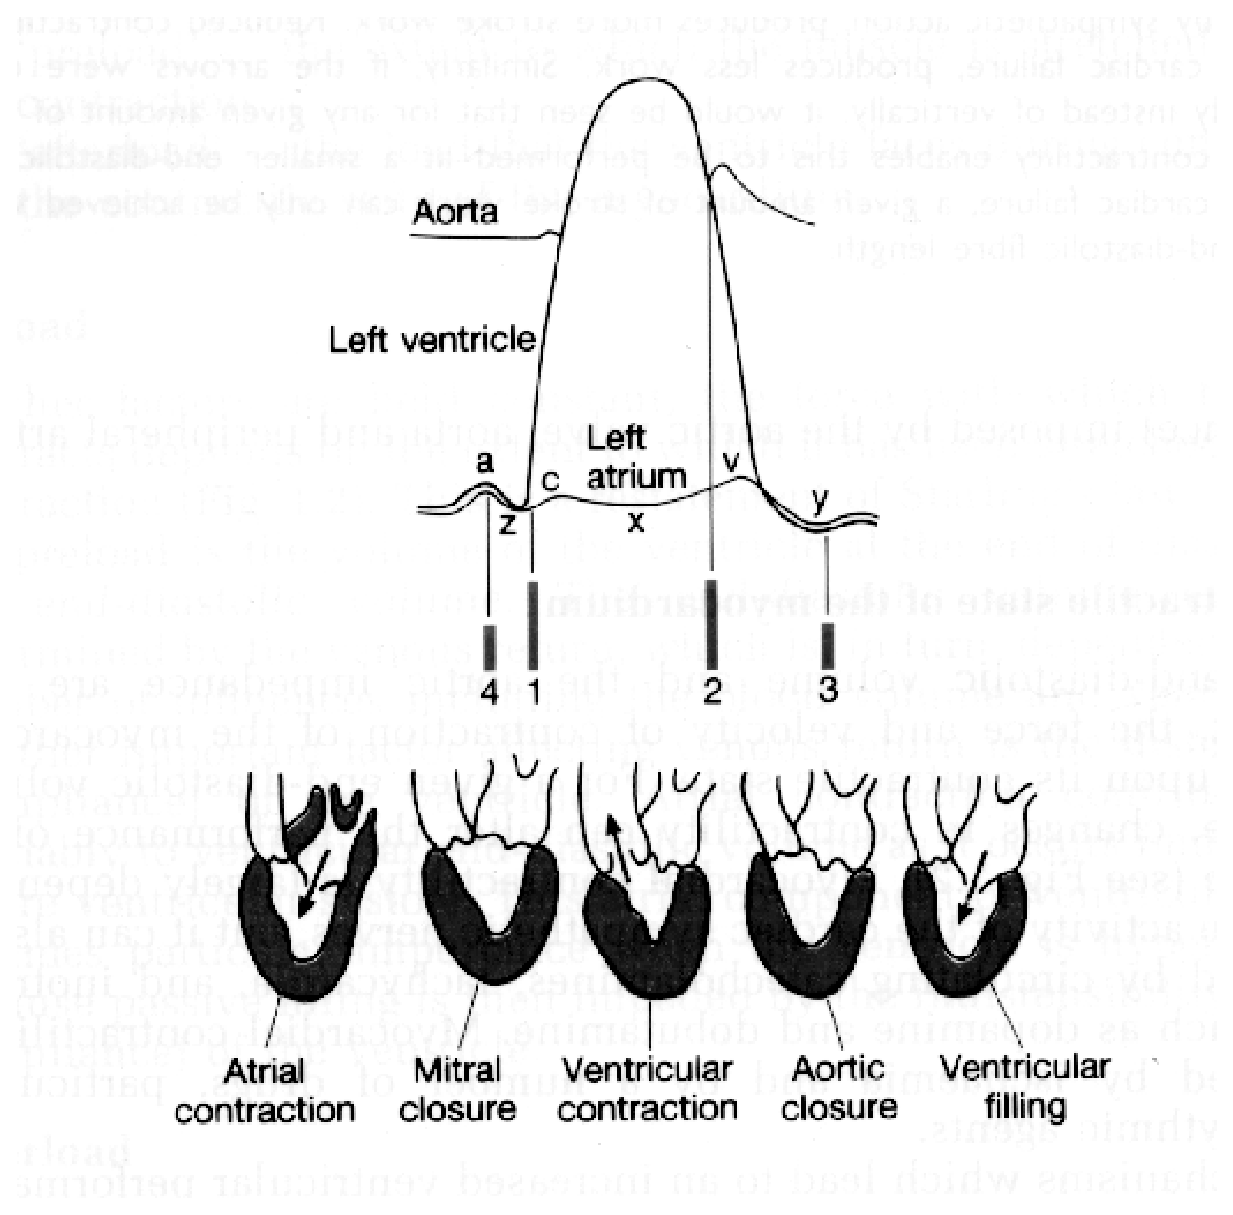
\epsfig{file=electrocardiology/epsfiles/press-vol2.eps,width=10cm}
  \caption{Pressure pulses in the left atrium, left ventricle and aorta}
  \label{fig:press-vol2}
\end{figure}

The relation between the pressure and the electrical impulse is shown in 
\figref{fig:press-vol}.
\begin{figure}[htbp] \centering
  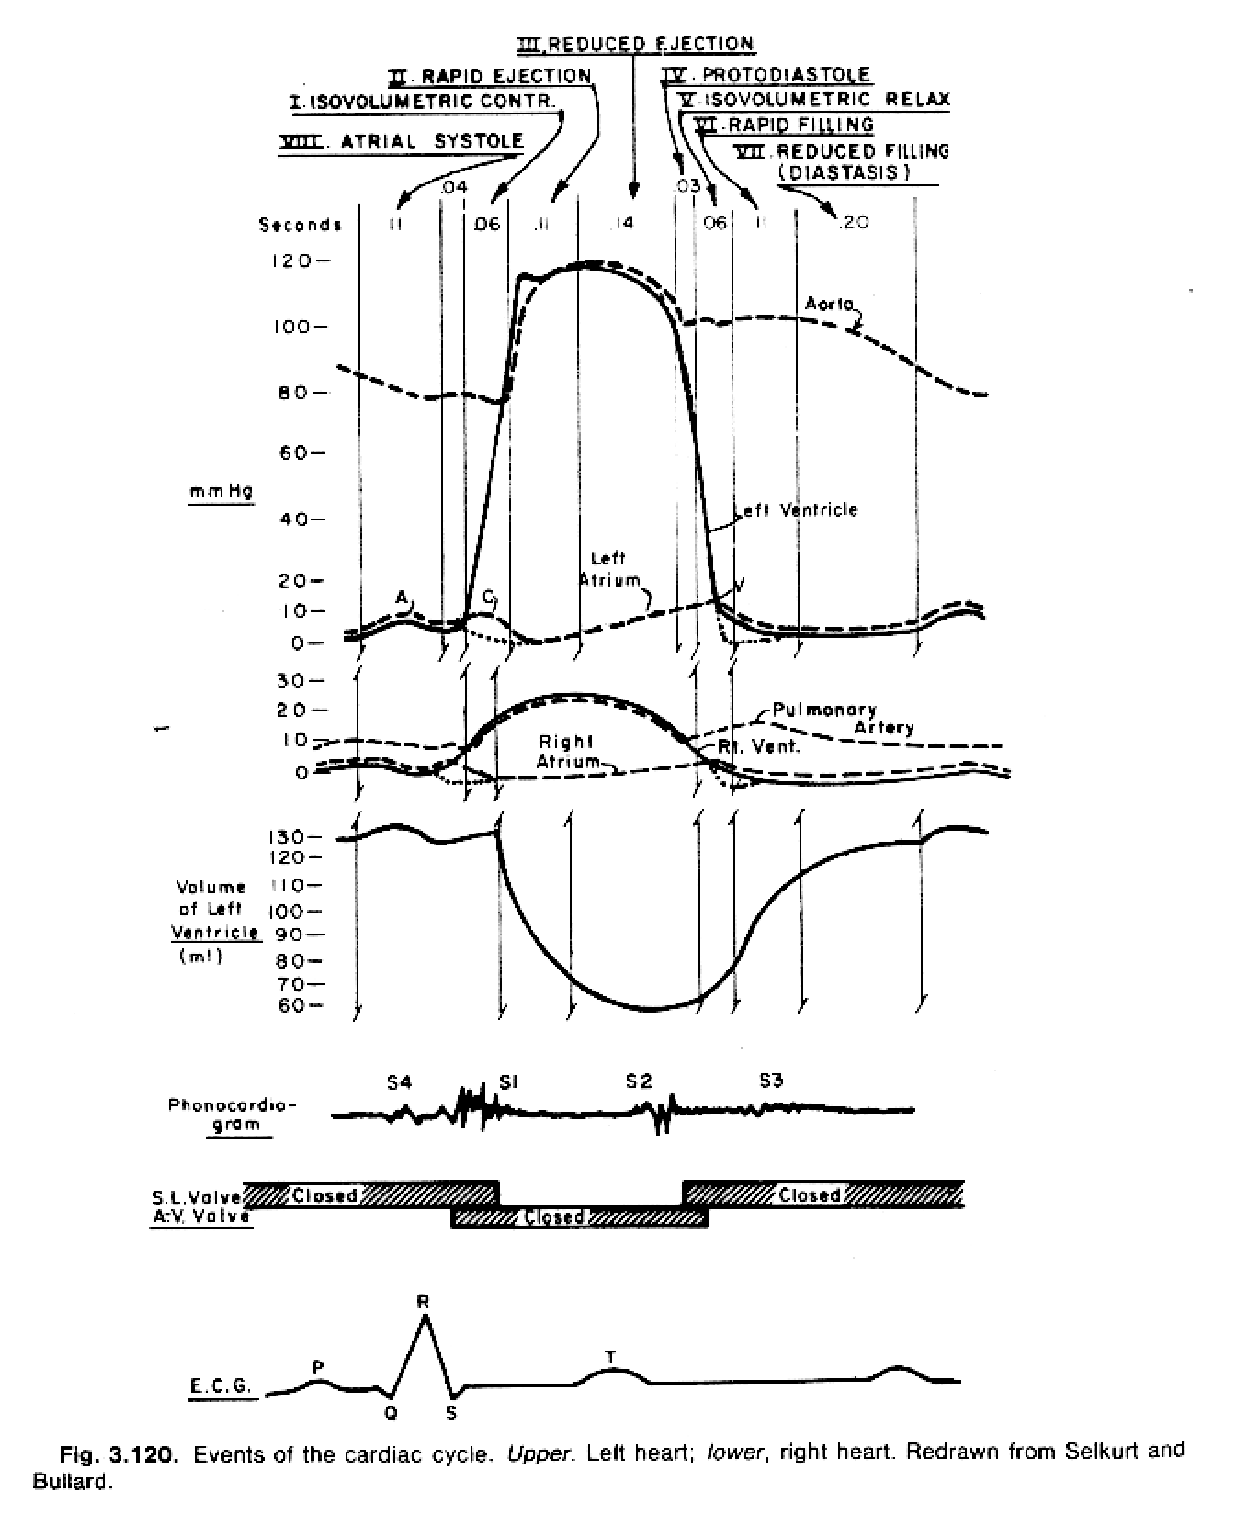
\epsfig{file=electrocardiology/epsfiles/press-vol.eps,width=10cm}
  \caption{Events of the cardiac cycle - pressure, volume and ECG}
  \label{fig:press-vol}
\end{figure}

\section{History of the ECG}
The bioelectric sources which arise during the heart's excitation process
produce a flow of electric current in the surrounding tissues.  It is
therefore possible to detect, with a pair of electrodes external to the heart,
time-varying potential differences known as electrocardiograms.

The first recording of a human ECG was by \citeasnoun{waller:1887}. The
electrical activity of the exposed heart was already known ( and galvanometers
had been invented) but Waller decided to investigate the possibility of
recording potentials from the limbs of animals and from man.  He dipped his
right hand and left foot into a couple of basins of salt solution which were
connected to two poles of an electrometer and ``at once had the pleasure of
seeing the mercury column pulsate with the pulsation of the heart''.

Waller demonstrated this at St Mary's Laboratory in 1887 and Professor Willem
Einthoven was in the audience (Waller often demonatrated the ECG on his dog
Jimmie standing in buckets of salt solution). It is Einthoven\footnote{Willem
  Einthoven was awarded the 1924 Nobel prize for Physiology or Medicine for
  the discovery of electrocardiogram mechanism} that most people credit with
the birth of the ECG (Einthoven acknowledges Waller as the first person to use
the word ECG) and Waller is overlooked.

Einthoven's major achievement was the invention of a device sensitive enough
to record \emph{potentials} from the body (as oppoesed to Waller who detected
\emph{voltages}).  Einthoven's first ECG machine weighed approximately 600
poinds and required 5 operators.

Einthoven is responsible for developing the theory on which the ECG is based
(e.g. Einthoven triangle, leads I, II, III, Einthoven equation). Einthoven's
notation for the ECG wave is still used.  A schematic ECG waveform is given in
\figref{fig:ECG}.  The letters P to U are used to denote certain parts of the
waveform and, as we will see in more detail later, they can be attributed to
different parts of the underlying cardiac activation.

\begin{figure}[htpb] \centering
  \input{electrocardiology/figs/ECG.pstex}
  \caption{`Standard' ECG (lead II waveform)}
  \label{fig:ECG}
\end{figure}

An ECG is recording (1) the spread of stimulus throught the heart muscle
(depolarisation) and (2) the return of the stimulated heart muscle to the
resting state (repolarisation).

\subsection{The Pathways of Conduction and the ECG}
As noted above, in the usual sequence of events, the electrical impulse arises in the sinus
node and spreads across the atria to reach the AV node. It can then only reach
the ventricles by passing into the rapidly conducting AV bundle and its
branches.

The first part of the ventricles to be activated is the septum, followed by
the endocardium.  Finally, the impulse spreads outwards to the epicardium.

The spread of the cardiac impulse gives rise to the main deflections of the
ECG: P, QRS and T waves.

\begin{itemize}
\item the \emph{P wave} is the first deflection of the cardiac cycle and
  represents atrial depolarisation;
\item the \emph{PR interval} represents the time taken for the cardiac impulse
  to spread over the atrium and through the AV node and His-Purkinje System;
\item the \emph{QRS complex} represents the spread of the depolarisation
  through the ventricles'
\item the\emph{T wave} represents the ventricular repolarisation.
\end{itemize}

There is still debate over the existence and interpretation of the U wave.

\subsection{Electrodes and Leads}
A conventional ECG consists of tracings from 12 leads. The
term `lead' refers to the ECG obtained as a result of recording the
difference in potential between a pair of electrodes.

\subsubsection{The bipolar (standard) leads} 
In these leads, the electrodes are
attached to the limbs. In lead I the positive electrode is attached to the
left arm  and the negative to the right arm. In lead II the positive
electrode is atttached to the left leg and the negative to the right arm.  In
lead III the positive is attached to the left leg and the negative to the
left arm. They may thus be depicted as :
\begin{itemize}
\item lead I = left arm minus right arm (LA -RA)
\item lead II = left leg minus right arm (LL-RA)
\item lead III = left leg minus left arm (LL-LA).
\end{itemize}
i.e.
\begin{eqnarray*}
  I & = & E_{L} - E_{R}\\
  II & = & E_{F} - E_{R}\\
  III & = & E_{F} - E_{L}
\end{eqnarray*}

These leads were the original leads that were used by Eintoven in his early
recordings. It can be deduced from these equations that lead II should be equal to the
sums of lead I and III i.e.
\begin{eqnarray*}
  I + III = II & & \mbox{(Einthoven's law)}
\end{eqnarray*}
.

Einthoven regarded each limb used in the recording of the bipolar ECG as an
apex of an equilateral triangle, equidistant electrically form the heart at
the centre\figref{fig:ET}. This idea is still used today in the interpretation
of ECGs, despite its obvious limitations (e.g. the body is not an electrically
homogenoeous sphere).

\begin{figure}[htpb] \centering
  \input{electrocardiology/figs/ET.pstex}
  \caption{Orientation of leads I,II,II - Eintovens triangle}
  \label{fig:ET}
\end{figure}


\subsubsection{Unipolar leads}
1934 saw the introduction of unipolar leads - so called because they represent
the potential variation of a single point.  In 1942 Goldberger modified these
to produce the so called augmented unipolar lead (done so the voltages were
easier to detect.
The unipolar leads have an exploring electrode placed on a chosen site linked with an
indifferent electrode with a very small potential. In an attempt to obtain a
central terminal with `zero potential', Wilson connected all three limb
electrodes through 5000 $\Omega $ resistances to form the indifferent
electrode.

\paragraph{Unipolar chest leads}
When unipolar leads are recorded from the chest wall, the exploring electrode
is connected to the positive pole of the ECG and the negative to the central
terminal. By convention, the following sites for the exploring electrode
 are normally selected (shown in\figref{fig:v1-v6}, \figref{fig:v1-v6-b}):
\begin{itemize}
\item V1, the fourth intercostal space just to the right of the sternum;
\item V2,  the fourth intercostal space just to the left of the sternum;
\item V3, midway between V2 and V4;
\item V4, the fifth intercostal space in th emidclavicular line;
\item V5, the left anterior axillary line at the same horizontal level as
  V4;
\item V6, the left mid-axillary line at the same horizontal level as V4
\end{itemize}

\begin{figure}[htbp] \centering
  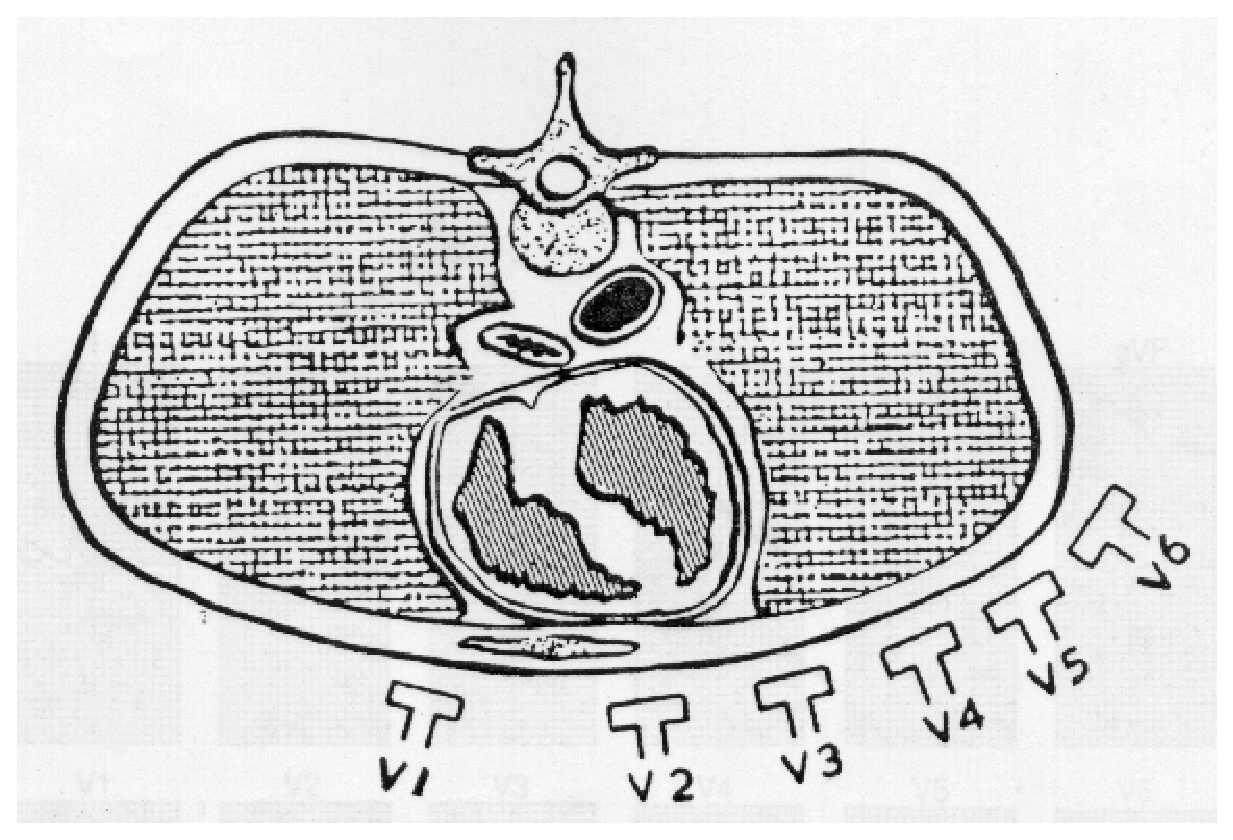
\epsfig{file=electrocardiology/epsfiles/v1-v6.eps,width=10cm}
  \caption{Diagram showing the orientation of the unipolar chest leads}
  \label{fig:v1-v6}
\end{figure}

\begin{figure}[htbp] \centering
  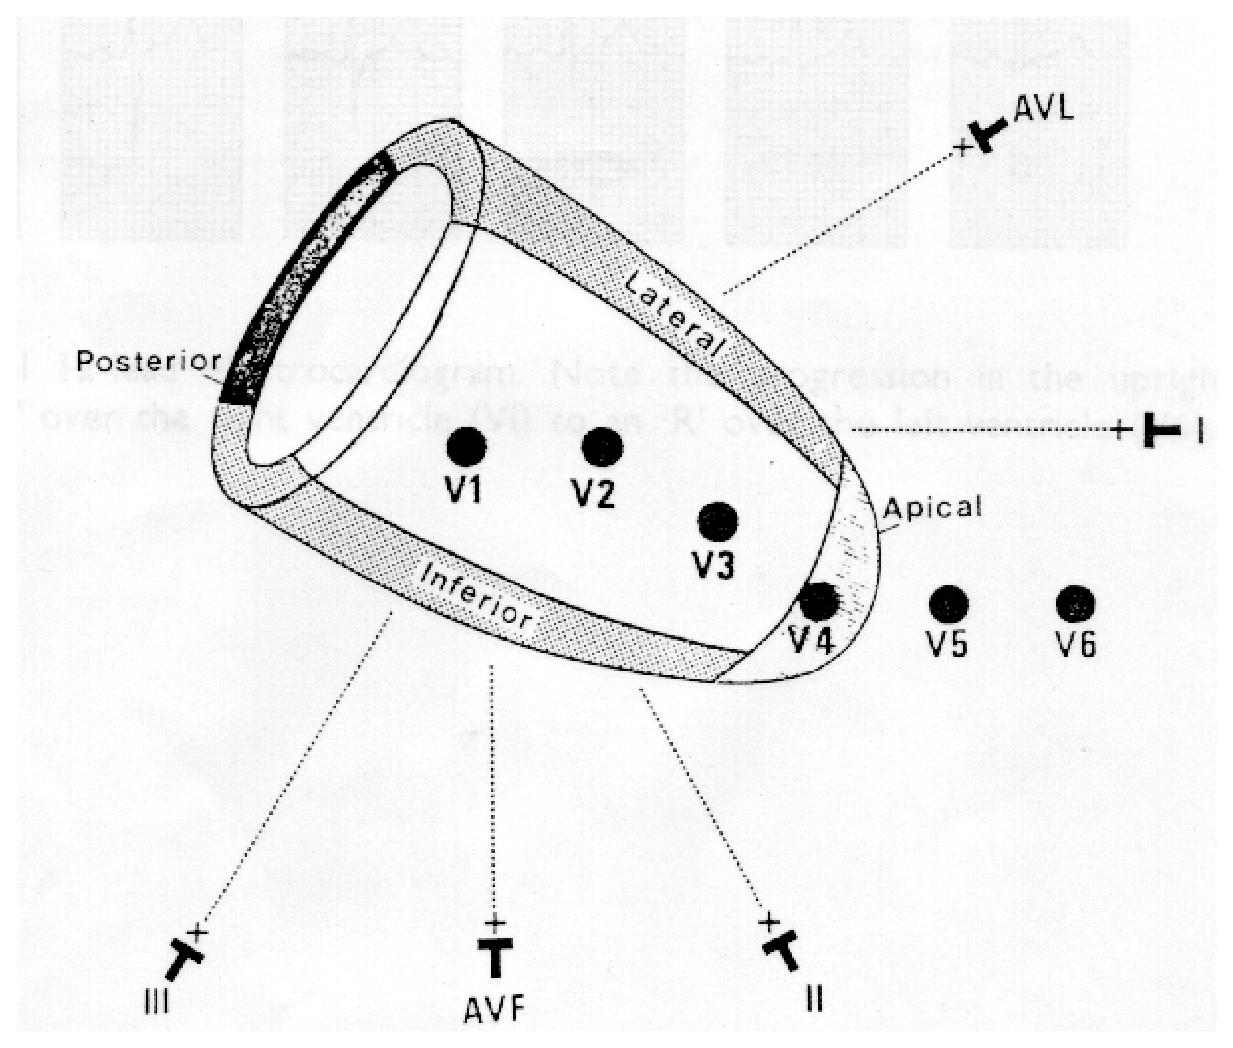
\epsfig{file=electrocardiology/epsfiles/v1-v6-b.eps,width=10cm}
  \caption{Diagram showing the orientation of the various leads to the left
    ventricular 'cone'.  Note that there is no lead which is oriented
    directly to the posterior wall of the heart}
  \label{fig:v1-v6-b}
\end{figure}

Additional leads can be taken from V3R and V4R, sites on the right side of
the chest equivalent to V3 and V4.  Occasionally, leads may be placed at
higher levels, e.g. the second, third or fourth intercostal spaces or
further laterally (V7 and V8).

\paragraph{Unipolar limbleads}
In these leads, the exploring electrode is placed on one limb, and the
negative pole is connected to Wilson's central terminal, modified by the
ommission of the connection from the limb under study to the central terminal
\figref{fig:ecg-leads}.

\begin{figure}[htbp] \centering
  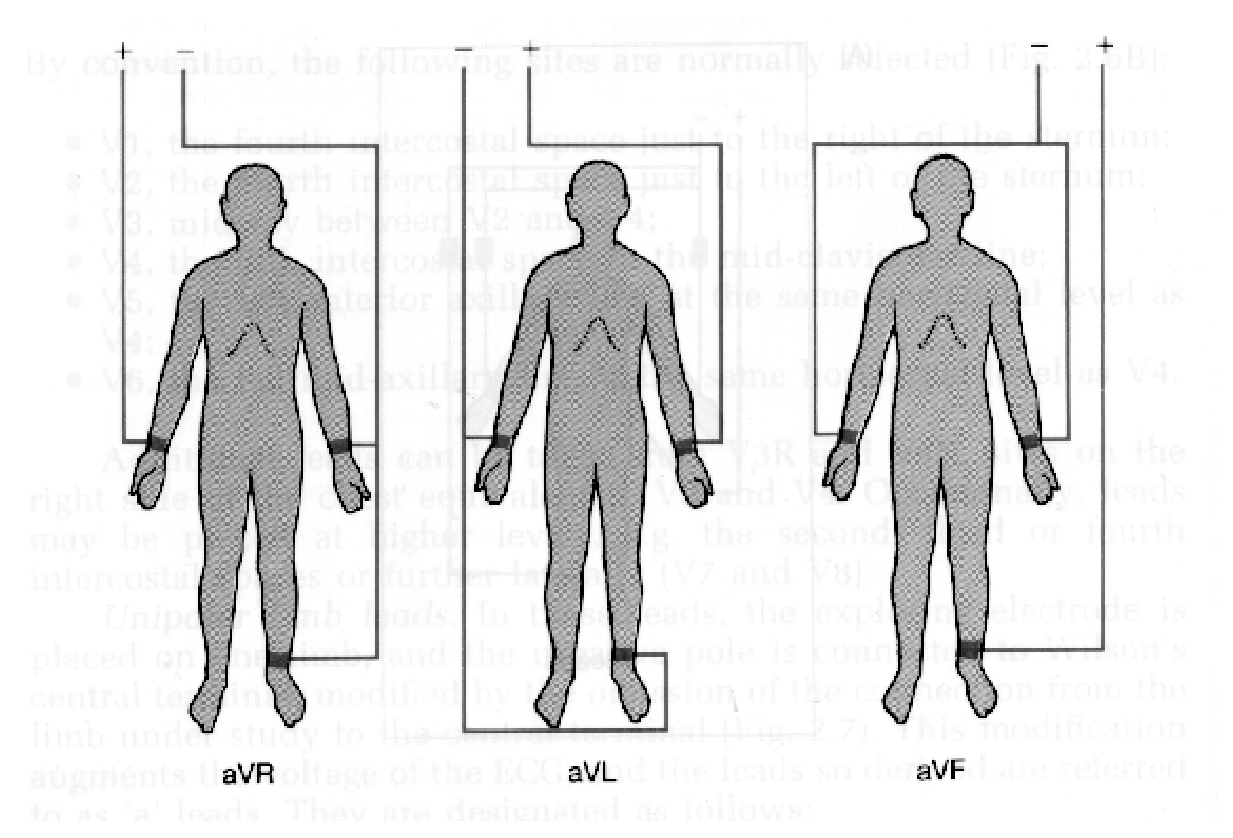
\epsfig{file=electrocardiology/epsfiles/ecgleads.eps,width=10cm}
  \caption{The attachment of unipolar limb leads.  Note that the limb under
    study is not attached to the central (negative) terminal}
  \label{fig:ecg-leads}
\end{figure}

This modification ``augments the voltage of the ECGs'', and the leads so derived
are referred to as 'a' leads. They are designated as follows:
\begin{itemize}
\item aVR, augmented voltage from the right arm;
\item aVL, augmented voltage from the left arm;
\item aVF, augmented voltage from the left foot.
\end{itemize}
If we consider each of these leads in a bit more detail then for aVR the
central terminal consists of the average of the voltages from L and F and aVR
is therefore
\begin{displaymath}
  aVR = E_{R} -\frac{1}{2} (E_{L} + E_{F} ) = -\frac{1}{2}(I + II)
\end{displaymath}
If an average of the potentials from V, L and F is used as the central
terminal (as in the original unipolar leads) then the voltage recorded, VR,
is only  $\frac{2}{3}aVR$ - hence the name ``augmented'' VR.
Similarly
\begin{eqnarray*}
  aVL = & E_{L} - \frac{1}{2} (E_{F} + E_{R}) & = I - \frac{1}{2} II\\
  aVF = & E_{F} - \frac{1}{2} (E_{L} + E_{R}) & = I \mp \frac{1}{2} I
\end{eqnarray*}
  
It can be seen, that once any 2 of the 6 extremity leads (I, II, III, aVR,
aVF, aVL) have been recorded the others can be deduced.

So the six extremity leads (I,I,II, aVR, aVL, aVF) show electrical voltage of
the heart transmitted onto a vertical plane while the 6 precordial leads show
voltages transmitted onto the horizontal plane.

\section{Basic Theory}

Einthoven's original model has proven extremely useful and still dominates
much of electrocardiography. Einthoven used a dipole to represent the heart
and postulated that the potentials at the limbs were related to the heart in
the same way that the potential at the 3 vertices of an equilateral triangle
places in an unbounded homogenous two dimensional volume conductor would be
related to a dipole source at the centre of the triangle. That is the heart
was modelled as a dipole and the body as part of a homogenous infinite
conductor.

More detailed models have been developed (taking into account inhomogeneities,
etc.) but the dipole model is still widely used (it is simple and reasonably
accurate).

The ECG shows \emph{projections} of this dipole in the direction of the leads.
At position 1, projection onto lead II is small and negative (Q wave). As the
``heart vector'' sweeps through positions 2,3 and 4 the projection onto lead
II is large and positive (the R complex). From 4 back to 0 the deflection
becomes small and negative (see \figref{fig:heart_vect_mb}).

\pstexfigure{electrocardiology/figs/HV.pstex}{}{Heart vector projections}{fig:heart_vect_mb}

More complicated models (which used quadrupoles, solid angles, etc.) give rise
to approximately the same thing.

The 12 different lead sites show the projection of the dipole along 12
different directions.


\section{The Normal ECG} 

\subsection{The Normal Electrocardiogram}
A normal 12 lead ECG recording is given in \figref{fig:normalecg}.  We discuss
below the significance of each part.
\subsubsection{The P Wave}
The normal P wave (\figref{fig:pwaves}~A) results from the spread of electrical activity across the
atria (the activity of the sinus node itself cannt be detected in the
ECG). Because the impulse spreads from right to left, the P wave is upright in
leads I,II and aVF, is inverted in aVR and may be upright, biphasic or
inverted in lead III,aVL and V1. It should not be higher than 3mm in the
bipolar leads or 2.5mm in the unipolar leads, or greater than 0.10 s in duration.

\begin{figure}[htbp] \centering
 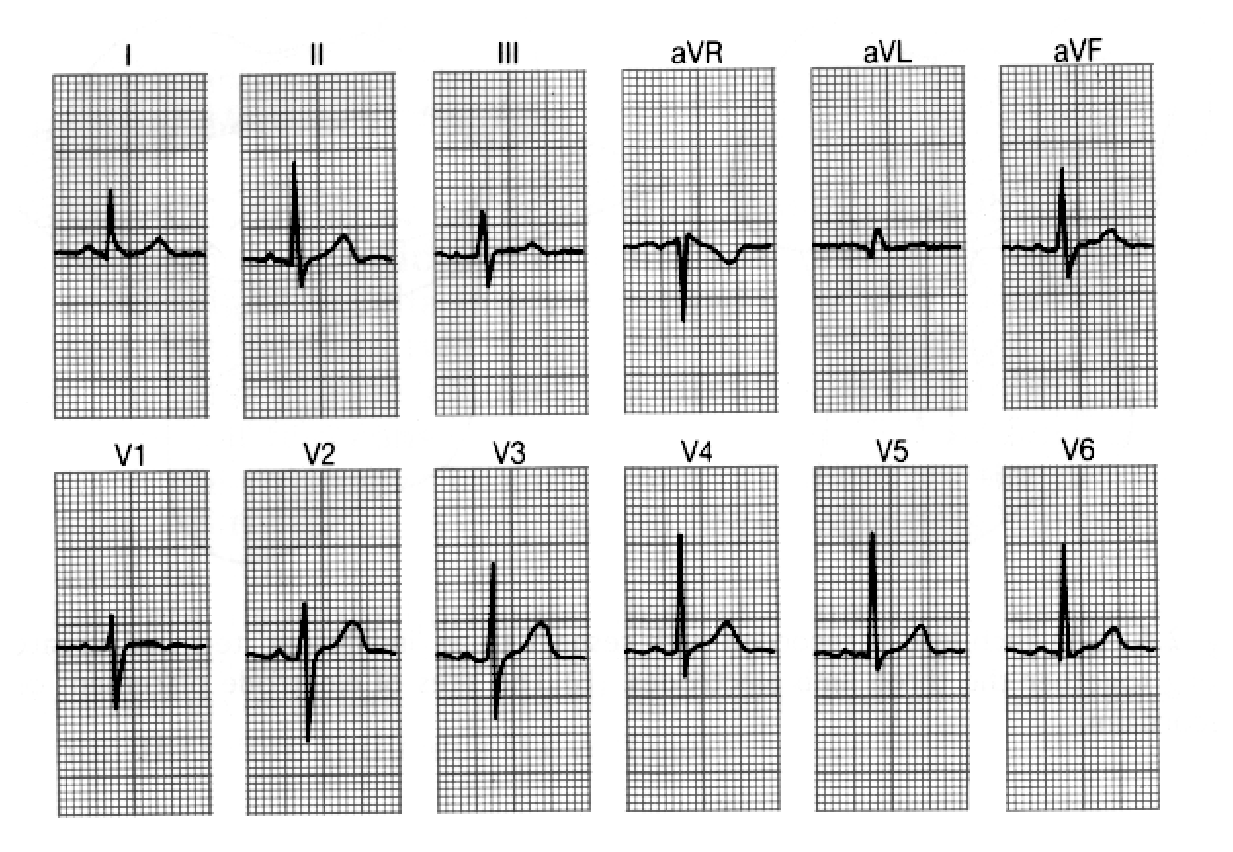
\epsfig{file=electrocardiology/epsfiles/normalecg.eps,width=10cm}
 \caption[Normal 12-lead electrocardiogram.]{Normal 12-lead
   electrocardiogram. Note the progression in the upright deflection from `r'
   over the right ventricle (V1) to an `R' over the left ventricle V6.}
 \label{fig:normalecg}
\end{figure}

\begin{figure}[htbp] \centering
 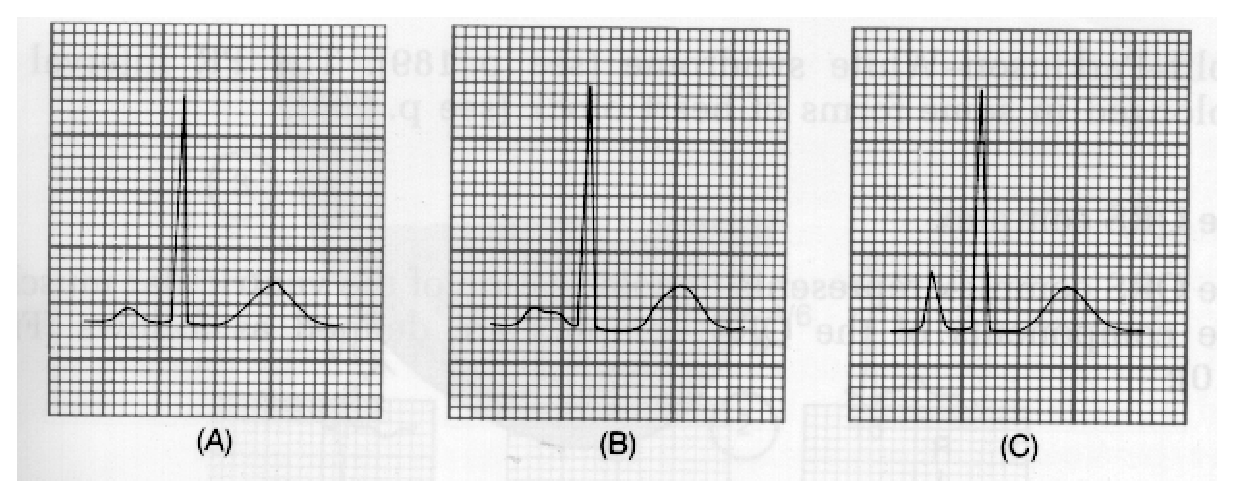
\epsfig{file=electrocardiology/epsfiles/pwaves.eps,width=10cm}
 \caption[P wave appearance in lead II.]{P wave appearance in lead II. (A) Normal. (B) Broadened and
   notched (P mitrale). (C) C Tall and peaked (P pulmonale).}
 \label{fig:pwaves}
\end{figure}

When abnormal (\figref{fig:pwaves}~B, C), the P wave may become:
\begin{itemize}
\item \emph{inverted} (i.e. negative in the leads in which it is usually
  positive). This indicates depolarisation of the atria in an unusual
  direction, and that the pacemaker is not in the sinus node, but situated
  either elsewhere in the atrium, in the AV node or below this; or there is dextrocardia;
\item \emph{broadened and notched}, due to delayed depolarisation of the left atrium
 when this chamber is enlarged (P mitrale) (\figref{fig:pwaves}~B). In  V1, the P wave is then
 usually biphasic with a small positive wave preceding a deep and broad
 negative one;
\item \emph{tall and peaked}, exceeding 3mm, as a result of right atrial
  enlargement (P pulmonale) (\figref{fig:pwaves}~C);
\item \emph{absent} or invisible due to the presence of junctional rhythm or
  sino-atrial block;
\item replaced by flutter or fibrillation waves.
\end{itemize}

\subsection{The PR Interval}
This is measured from the beginning of the P wave to the beginning of the QRS
complex (i.e. to the onset of the Q wave if there is one, and to the onset of
the R wave if there is not).  This interval corresponds to the time taken for
the impulse to travel from the sinus node to the ventricular muscle. There is an iso-electric segment
between the end of the P wave and the beginning of the QRS complex, whilst the
impulse is passing through the AV node and specialised
conducting tissue, as an insufficient amount of tissue is being electrically
stimulated to produce a deflection detectable on the body surface.

The PR interval varies with age and with heart rate. The upper limit in
children is 0.16, in adolescents 0.18 and in adults 0.20s, although it may be
even longer in a few normal individuals. The faster the heart rate the shorter
is the PR interval. It is regarded as abnormally short if it is less than
0.01s. A shortened PR interval is seen when the impulse originates in the
junctional tissues and in the Wolff-Parkinson-White syndrome (see later).
 The PR interval
is prolonged in some forms of heart block.

\subsubsection{The QRS Complex}
The QRS complex represents depolarisation of ventricular muscle. The
components of the QRS complex are defined as follows
(figure~\ref{fig:qrs}:

\begin{figure}[htbp] \centering
  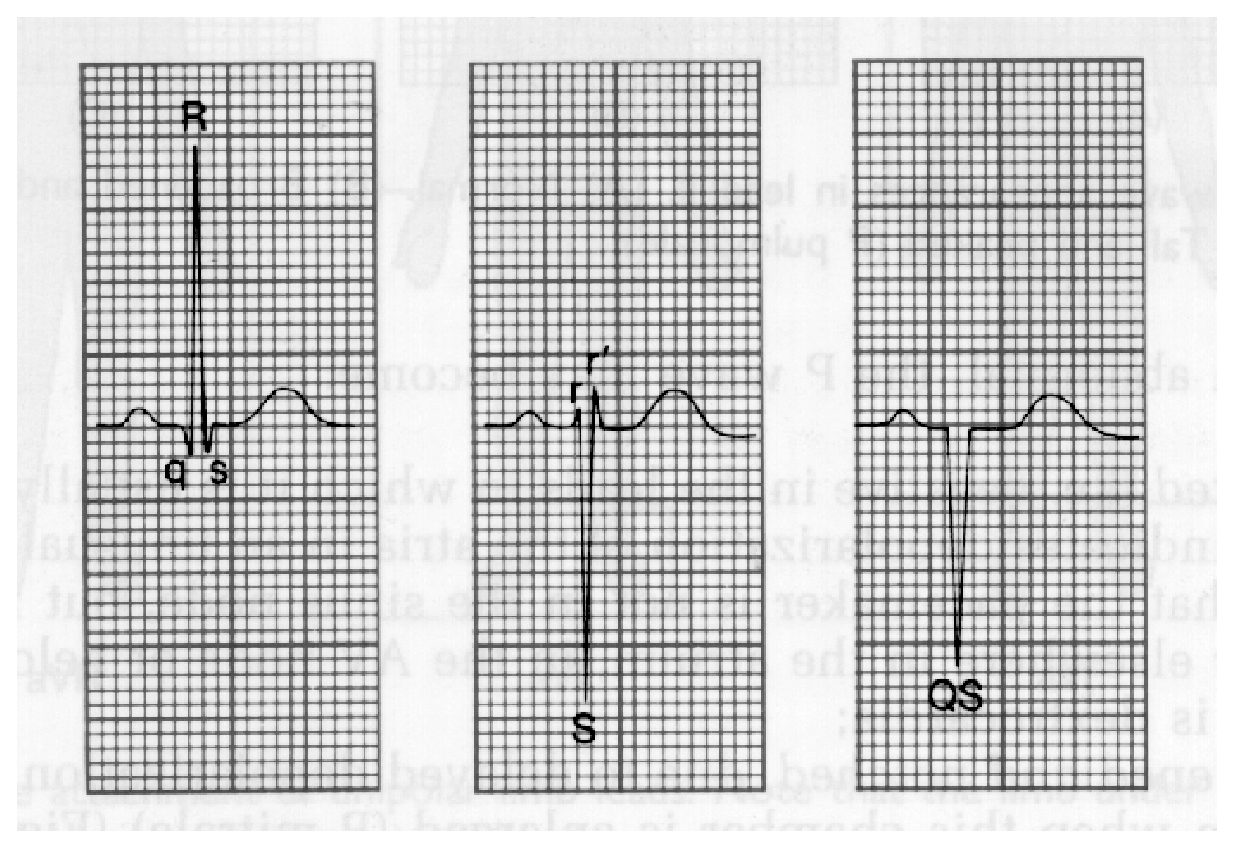
\epsfig{file=electrocardiology/epsfiles/qrs.eps,width=10cm}
 \caption[Variations in the QRS complex]{Variations in the QRS complex (see text)}
  \label{fig:qrs}
\end{figure}

\begin{itemize}
 \item the R wave is any positive(upward) deflection of QRS complex. If there
  is more than one R wave, the second is denoted R'; and R wave of small
  voltage may be denoted r; 
 \item a negative (downward) deflection preceding an R wave is termed Q;
 \item a negative (downward) deflection following an R wave is termed S
 \item if the ventricular complex is entirely negative (i.e. there is no R
  wave), the complex is termed QS.
\end{itemize}

The whole complex is often referred to as the QRS complex irrespective of
whether one or two of its components are absent.

Ventricular depolarisation starts in the middle of the left side of the septum
and spreads across to the right (phase 1 of ventricular depolarisation)
(Figure~\ref{fig:heartqrs}). Subsequently, the main free walls of the
ventricles are activated, the impulse spreading from within outwards and from
below upwards. Because of the dominating bulk of the left ventricle, the
direction of the vector of phase 2 is to the left and posteriorly. Finally,
the base of both ventricular walls and the interventricular septum are
depolarised. The appearances of the QRS in different leads can be largely
explained by the major vectors of these phases as seen in Figure
~\ref{fig:heartqrs}. In leads facing the left ventricular surface, there is a
small Q wave due to septal depolarisation and a large R wave due to left
ventricular depolarisation. On the right side of the heart, as seen by V1,
there is usually an r wave due to septal depolarisation and a large S wave
due to left ventricular forces directed away from the electrode.

\begin{figure}[htbp] \centering
  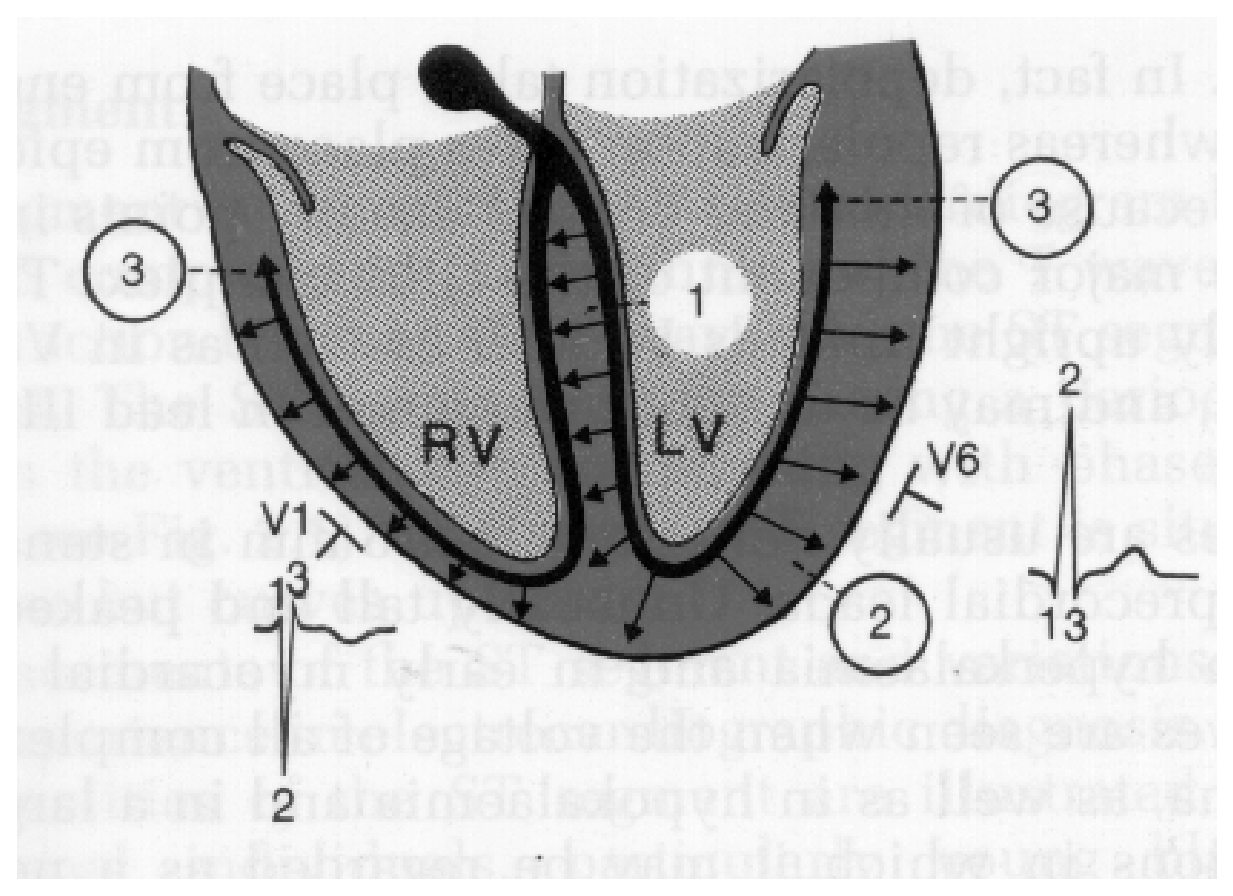
\epsfig{file=electrocardiology/epsfiles/heartqrs.eps,width=10cm}
 \caption[Genesis of QRS complex.]{Genesis of QRS complex. Note that the first phase, directed from
   left to right across the septum, produces a Q wave in $V6$ and an R wave in
   V1. The second phase, due mainly to depolarisation of the left ventricle
   from endocardium to epicardium, results in a tall R wave in V6 and a deep
   S wave in V1. Finally, depolarisation of the basal parts of the
   ventricles may produce a terminal S wave in V6 and a terminal R wave in V1}
  \label{fig:heartqrs}
\end{figure}

\paragraph{Pathological Q waves}
As mentioned, small, narrow Q waves are normally to be found in leads facing
the left ventricle, e.g. lead I, aVL, aVF, V5 and V6. These Q waves do not
normally exceed 2mm in depth, or 0.03s in width. It should be noted that QS
waves are normal in aVR, and are common in V1. Abnormally broad and deep Q
waves are often a feature of myocardial infarction. Q waves in lead III are
difficult to evaluate but can be ignored if there are no Q waves either in
lead II or in aVF, or if they do not exceed 0.03s. Usually a `normal' Q
wave in lead III diminishes or disappears on deep inspiration because of an
alteration in the position of the heart, whilst the `pathological' Q wave of
infarction persists.

The QRS complex should not exceed 0.10s duration, and usually is in the range
0.06-0.08s. Broad QRS complexes occur in bundle branch block, in ventricular
hypertrophy and in ventricular ectopic beats.

\subsubsection{The T Wave}

The T wave is due to depolarisation of the ventricles.  If repolarisation (the
T wave) occurred in the
same direction as depolarisation (the QRS complex) the T wave would be
directed in an opposite way to that of the QRS
complex. In fact, depolarisation takes place from endocardium to epicardium,
whereas repolarisation takes place from the epicardium to endocardium. Because
of this, the T wave usually points in the same direction as the major
component of the QRS complex. Thus, the T wave is normally upright in leads
I and II as well as in V3 to V6, is inverted in aVR, and may be
upright or inverted in lead III, aVL, aVF and V1 and V2.

The T waves are usually not taller than 5m in standard leads and 10mm in
praecordial leads. Unusually tall and peaked T waves may be seen in
hyperkalaemia and in early myocardial infarction. Flattened T waves are seen
when the voltage of all complexes is low, as in myxoedema, as well as in
hypokalaemia and in a large number of other conditions in which it may be
regarded as a non-specific abnormality. Slight T wave inversion is also often
non-specific , and may be due to such influences as hyperventilation, posture
and smoking. The most important casuses of T wave inversion are:
\begin{itemize}
\item myocardial ischaemia and infarction;
\item ventricular hypertrophy;
\item bundle branch block.
\end{itemize}

\subsubsection{The QT Interval}

The QT interval represents the total time from the onset of ventricular
depolarisation to the completion of repolarsation. It is measured from the
beginning of the Q wave (or R wave if there is no Q wave) to the end of the T
wave. Its duration varies with heart rate, becoming shorter as the heart rate
increases. In general, the QT interval at heart rates between 60 and 90 per
minute does not exceed in duration half the preceding PR interval. The
measurement of the QT interval is often difficult as the end of the T wave
cannot always be clearly identified, and the relationship between heart rate
and duration of the QT interval is a complex one. Tables are available in
textbooks of electrocardiography giving normal QT intervals. In practice, the
main importace of a prolonged QT interval is that it is associated with a risk
of ventricular tachycardias (particularly torsades de pointes), and sudden
death. A long QT is sometimes an inherited abnormality but may result from
such drugs as quinidine, procainamide, disopyramide, amiodarone and tricyclic
antidepressants.

\subsubsection{The ST Segment}
The ST segment is that part of the electrocardiogram between the end of the
QRS complex and beginning of the T wave. The point of junction between the S
wave and the ST segment is known as the J point. The ST segment occurs during
the period of unchanging polarity in the ventricles, corresponding with phase
2 of the action potential. The normal ST segment is situated on the
iso-electric line but curves upwards.

Displacements of the ST segment and variations in its shape are of great
importance in electrocardiographic diagnosis. ST segment elevation occurs because repolarisation of the injured tissue
occurs more rapidly than that of normal tissue and a potential gradient
exists.

\begin{tabular}{lp{10cm}}
ST elevation is caused by &-~ acute myocardial infarct (dead tissue with
injured tissue surrounding it)\\
 &-~pericarditis (inflammation of the pericardium\\
 &-~ventricular hypertrophy (enlarged ventricle)\\
 &-~myocardial ischaemia (detected as ST depression) (deficiency of blood to
part of the myocardium) can lead to myocardial infarcts\\
 &-~sinus tachycardia (fast heart beat, $>$100/ min, with its origin in the
 sinus node
\end{tabular}


\subsection{The U Wave}
The U wave is a broad, low-voltage wave present in most normal ECGs. Its cause
is unknown; it may become unusually prominent in hypokalaemia and with
digitalis therapy.

\subsection{Some Abnormal ECGs} 
%(see handouts 3-7)

Names of clinical conditions:
\begin{itemize}
\item Left ventricular hypertrophy %(figure missing)
\item Right ventricular hypertrophy \figref{fig:rvhypertrophy}
\item Left bundle branch block \figref{fig:leftbbb-ecg} 
(Purkinje fibres in the LV are interrupted \figref{fig:leftbbb} )
\item Right bundle branch block \figref{fig:rightbbb-ecg} 
(Purkinje fibres in the RV are interrupted \figref{fig:rightbbb} )
\item WPW (Wolff-Parkinson-White syndrome)
\end{itemize}

\begin{figure}[htbp] \centering
  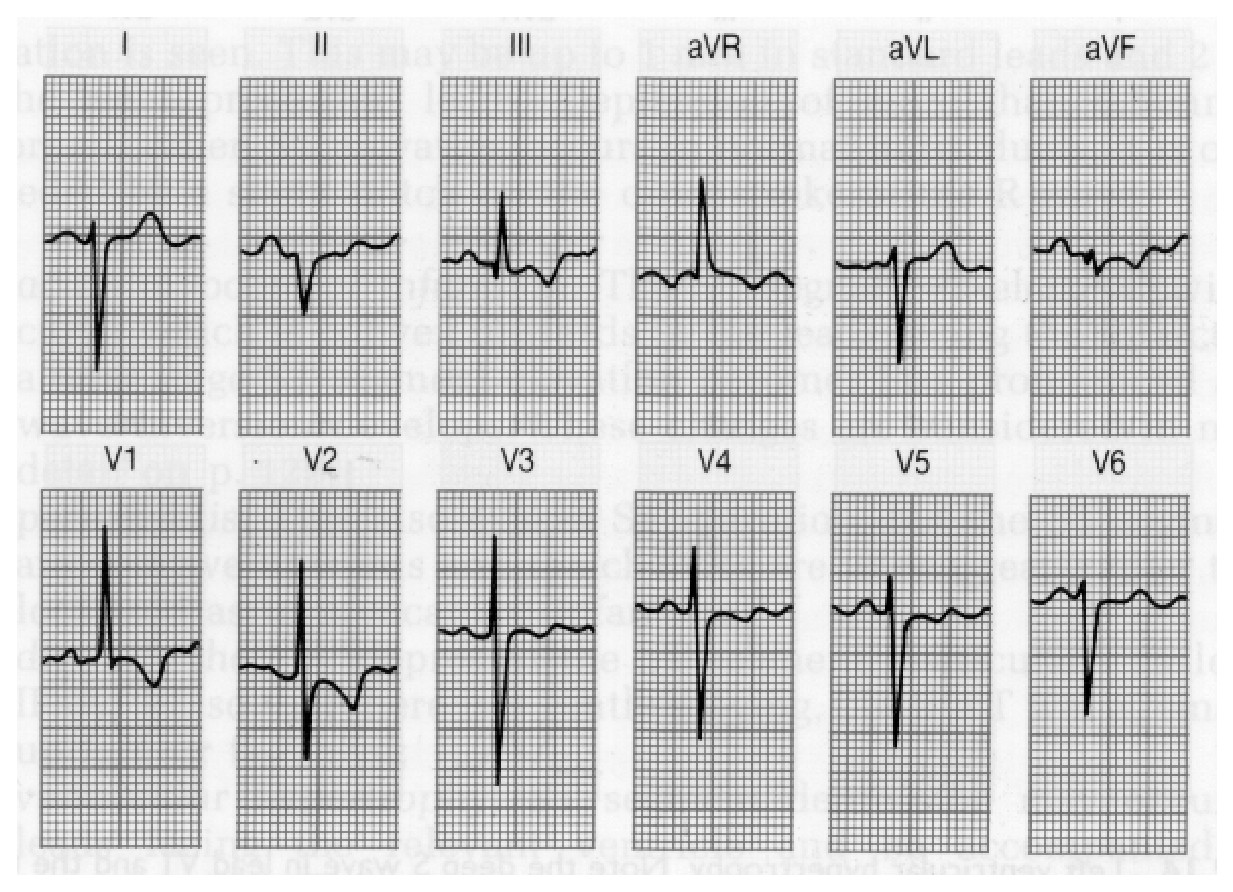
\epsfig{file=electrocardiology/epsfiles/rvhypertrophy.eps,width=10cm}
  \caption[Right Ventricular Hypertrophy]{Right Ventricular Hypertrophy.  Note
    the deep S wave in lead VI and the tall R waves in lead V5 and V6}
  \label{fig:rvhypertrophy}
\end{figure}

\begin{figure}[htbp] \centering
  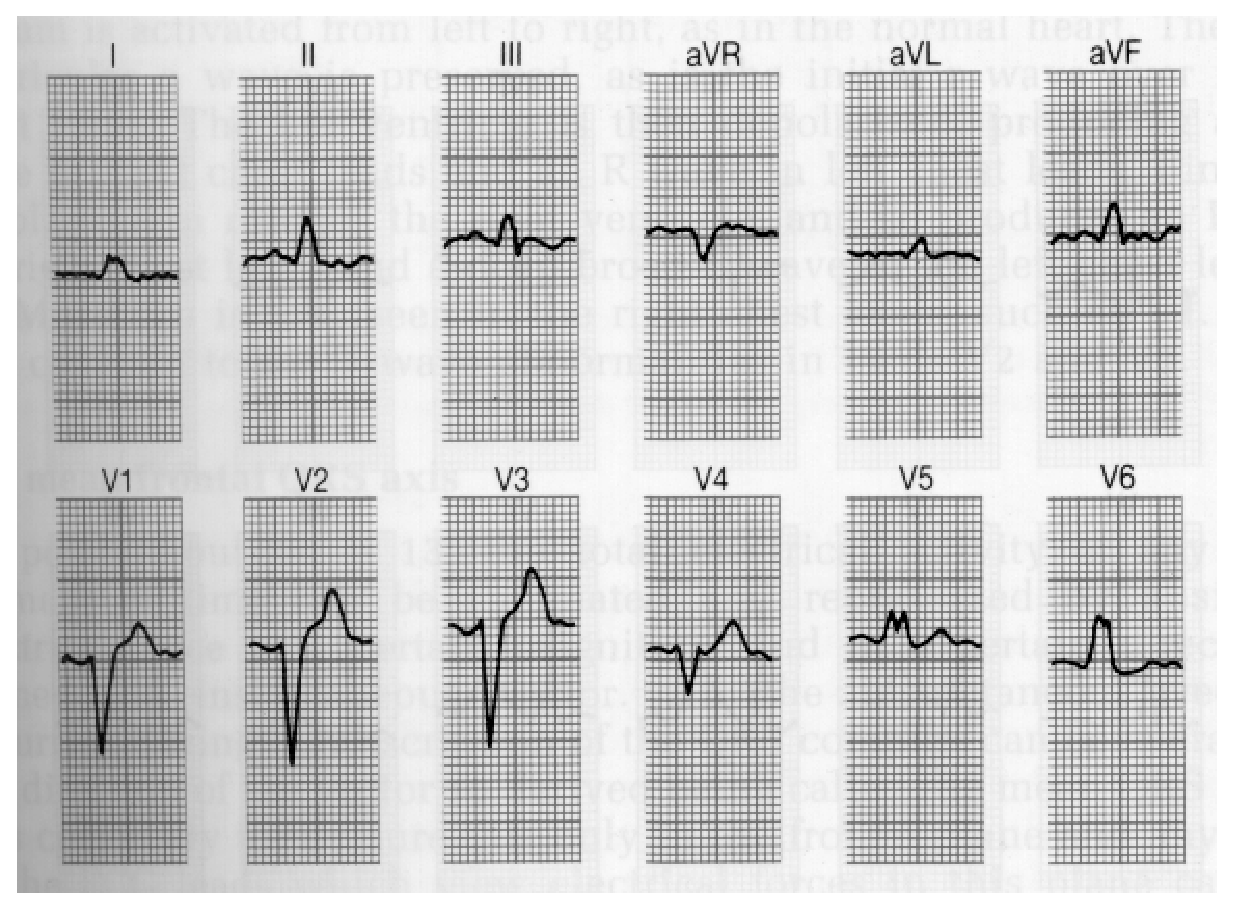
\epsfig{file=electrocardiology/epsfiles/leftbbb-ecg.eps,width=10cm}
  \caption[Left Bundle Branch Block ECG]{Left Bundle branch block ECG}
  \label{fig:leftbbb-ecg}
\end{figure}

\begin{figure}[htbp] \centering
  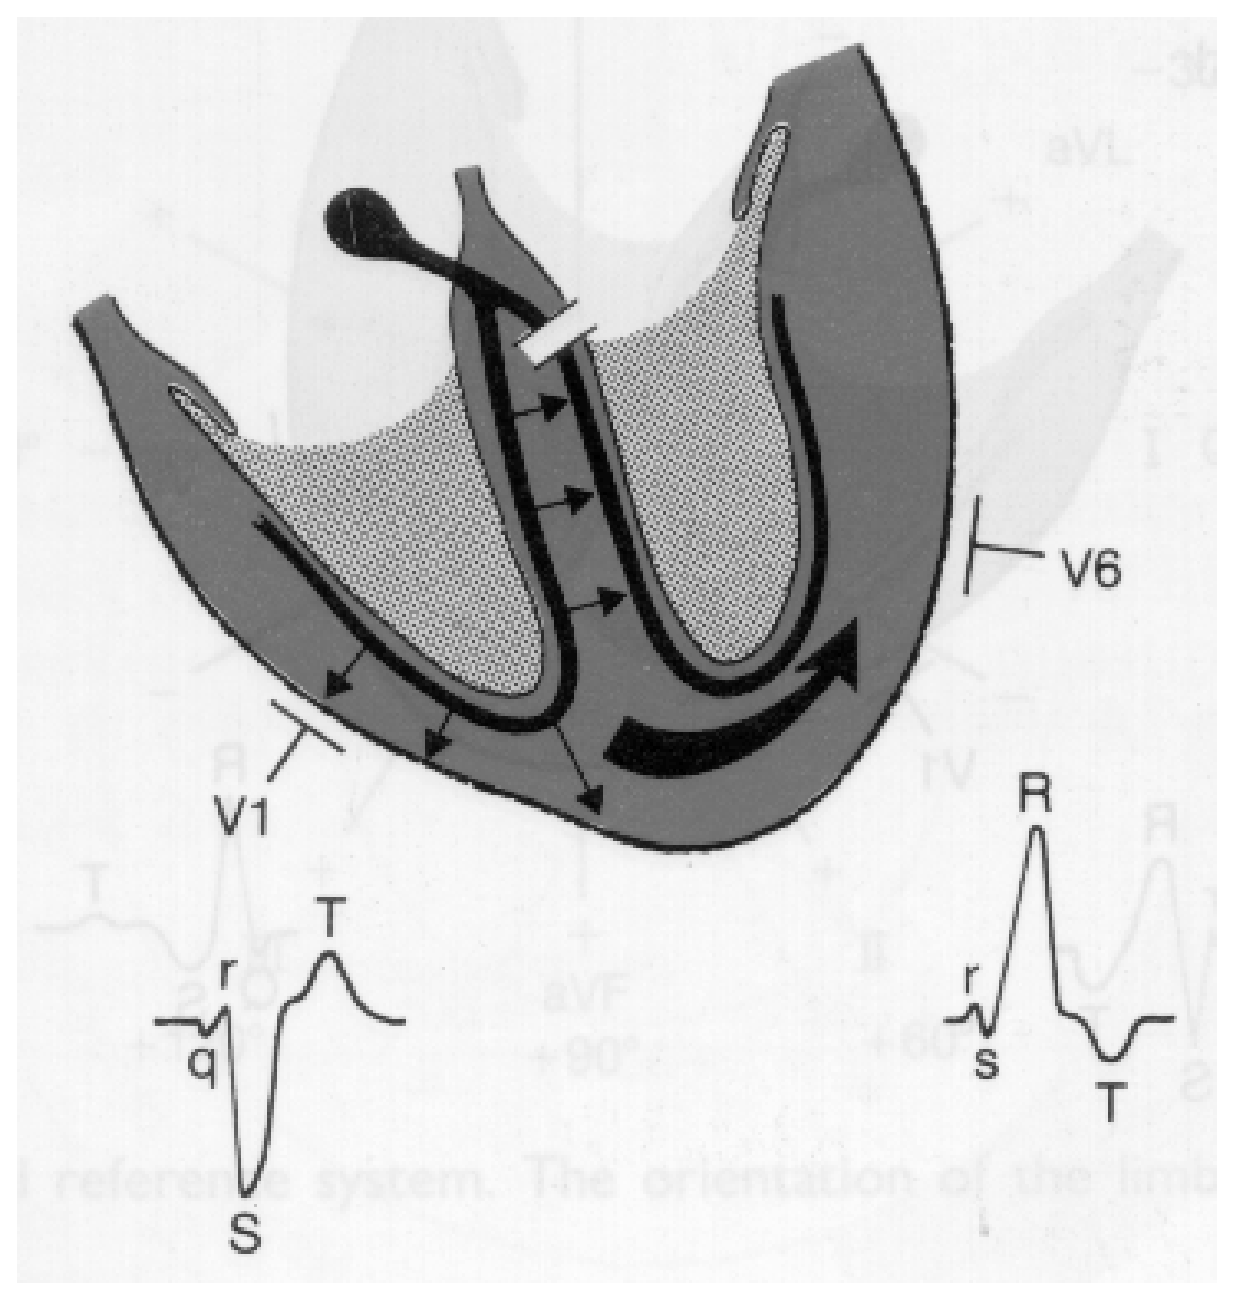
\epsfig{file=electrocardiology/epsfiles/leftbbb.eps,width=10cm}
  \caption[Left Bundle Branch Block]{Left Bundle Branch Block.  The inital
    vector is abnormal in being from right to left in the septum, thus
    producing an initial R wave in V6 and a Q wave in V1}
  \label{fig:leftbbb}
\end{figure}

\begin{figure}[htbp] \centering
  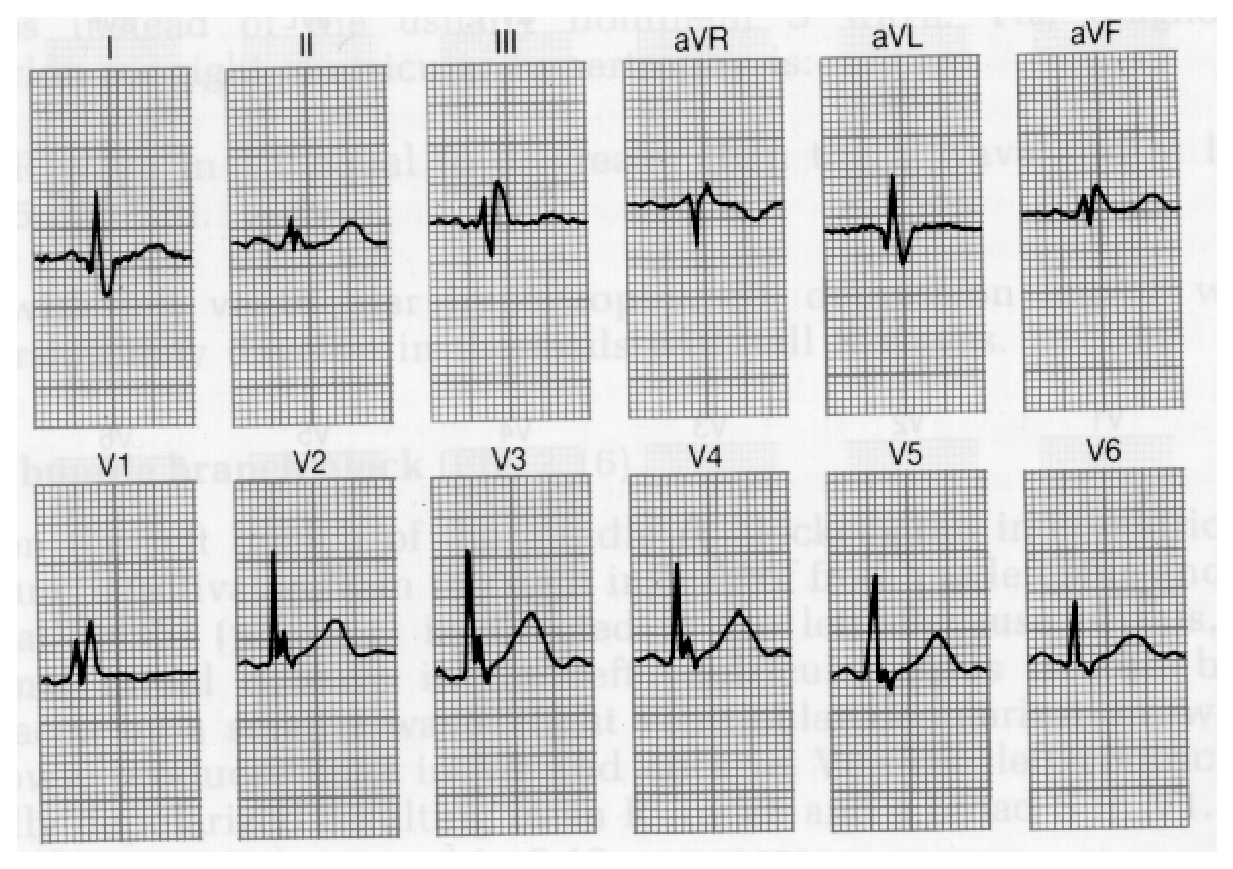
\epsfig{file=electrocardiology/epsfiles/rightbbb-ecg.eps,width=10cm}
  \caption[Right Bundle Branch Block ECG]{Right Bundle branch block ECG}
  \label{fig:rightbbb-ecg}
\end{figure}

\begin{figure}[htbp] \centering
  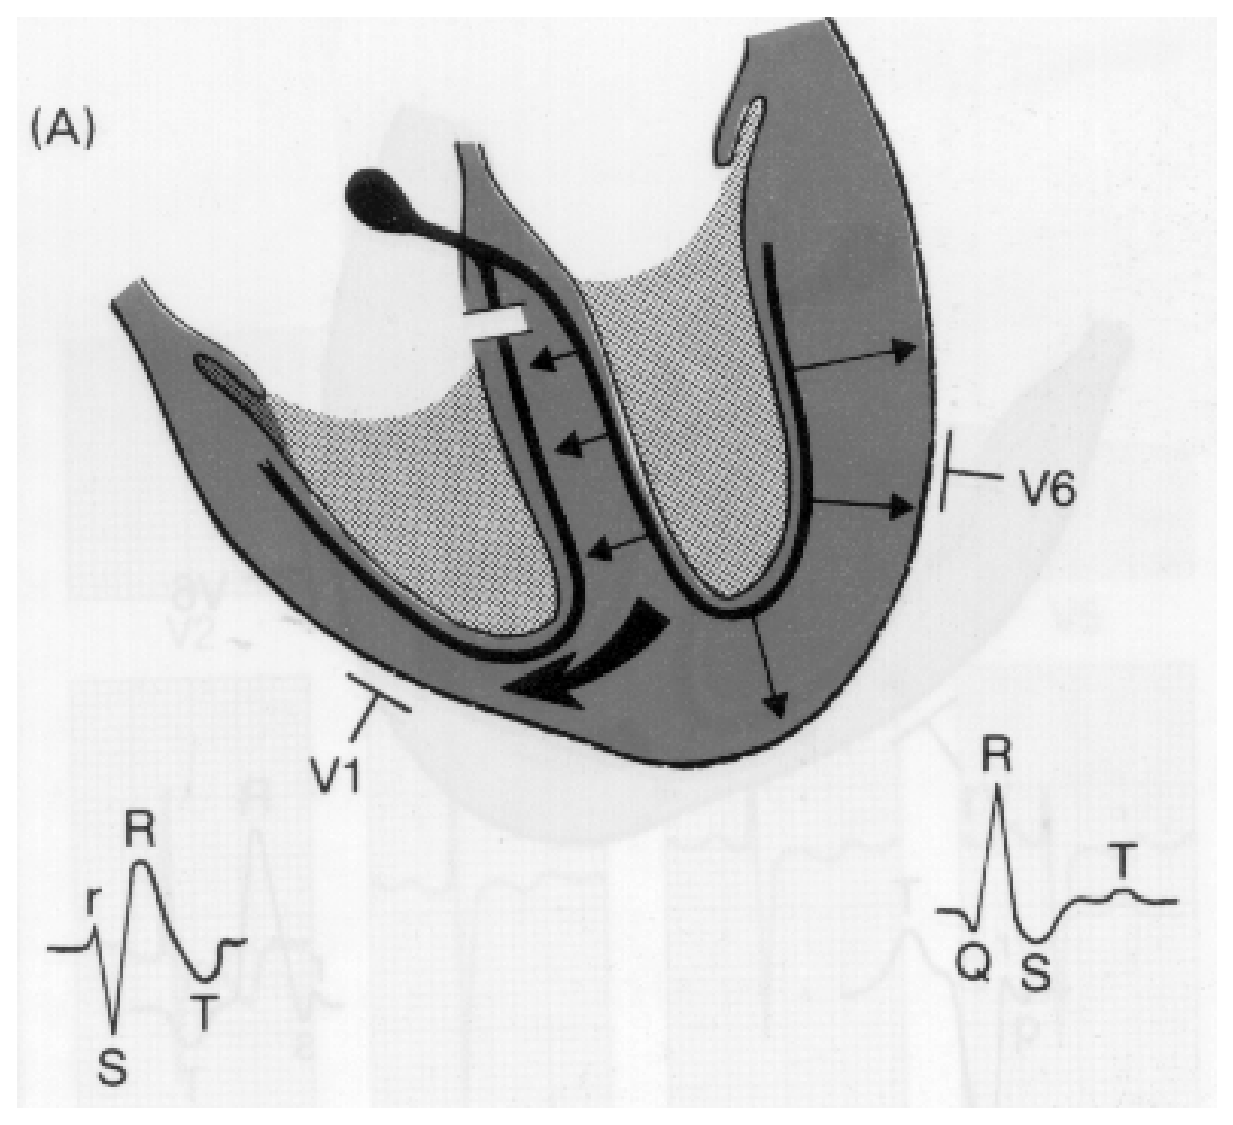
\epsfig{file=electrocardiology/epsfiles/rightbbb.eps,width=10cm}
  \caption[Right Bundle Branch Block]{Right Bundle Branch Block.  The septum
    is depolarised normally from left to right and hence a small Q is
    present in left ventricular leads and a small R in right ventricular
    leads.  Left ventricular depolarisation causes an S wave in V1 and an R
    wave in V6.  Late depolarisation of the right ventricle results in a
    prominent R' wave in V1 and broad S wave in V6}
  \label{fig:rightbbb}
\end{figure}

What can happen?

\noindent Ventricular Tachycardia (VT) - caused by slow conduction, or
presence of an infarct. This can lead to Ventricular Fibrillation (VF) where
there is no discernable pattern.  Death quickly follows if this is not
treated. %see ER!!! 

\begin{tabular}{lcp{13cm}}
Treatment &-&external defibrillation\\
          &-&internal defibrillator (implantable, onto heart, lasts
          about 4 years)
\end{tabular}

The strengths and limitations of the various treatments for ventricular
tachyarrhythmias is given in \figref{fig:tachy-arryth}.

\begin{figure}[htbp] \centering
  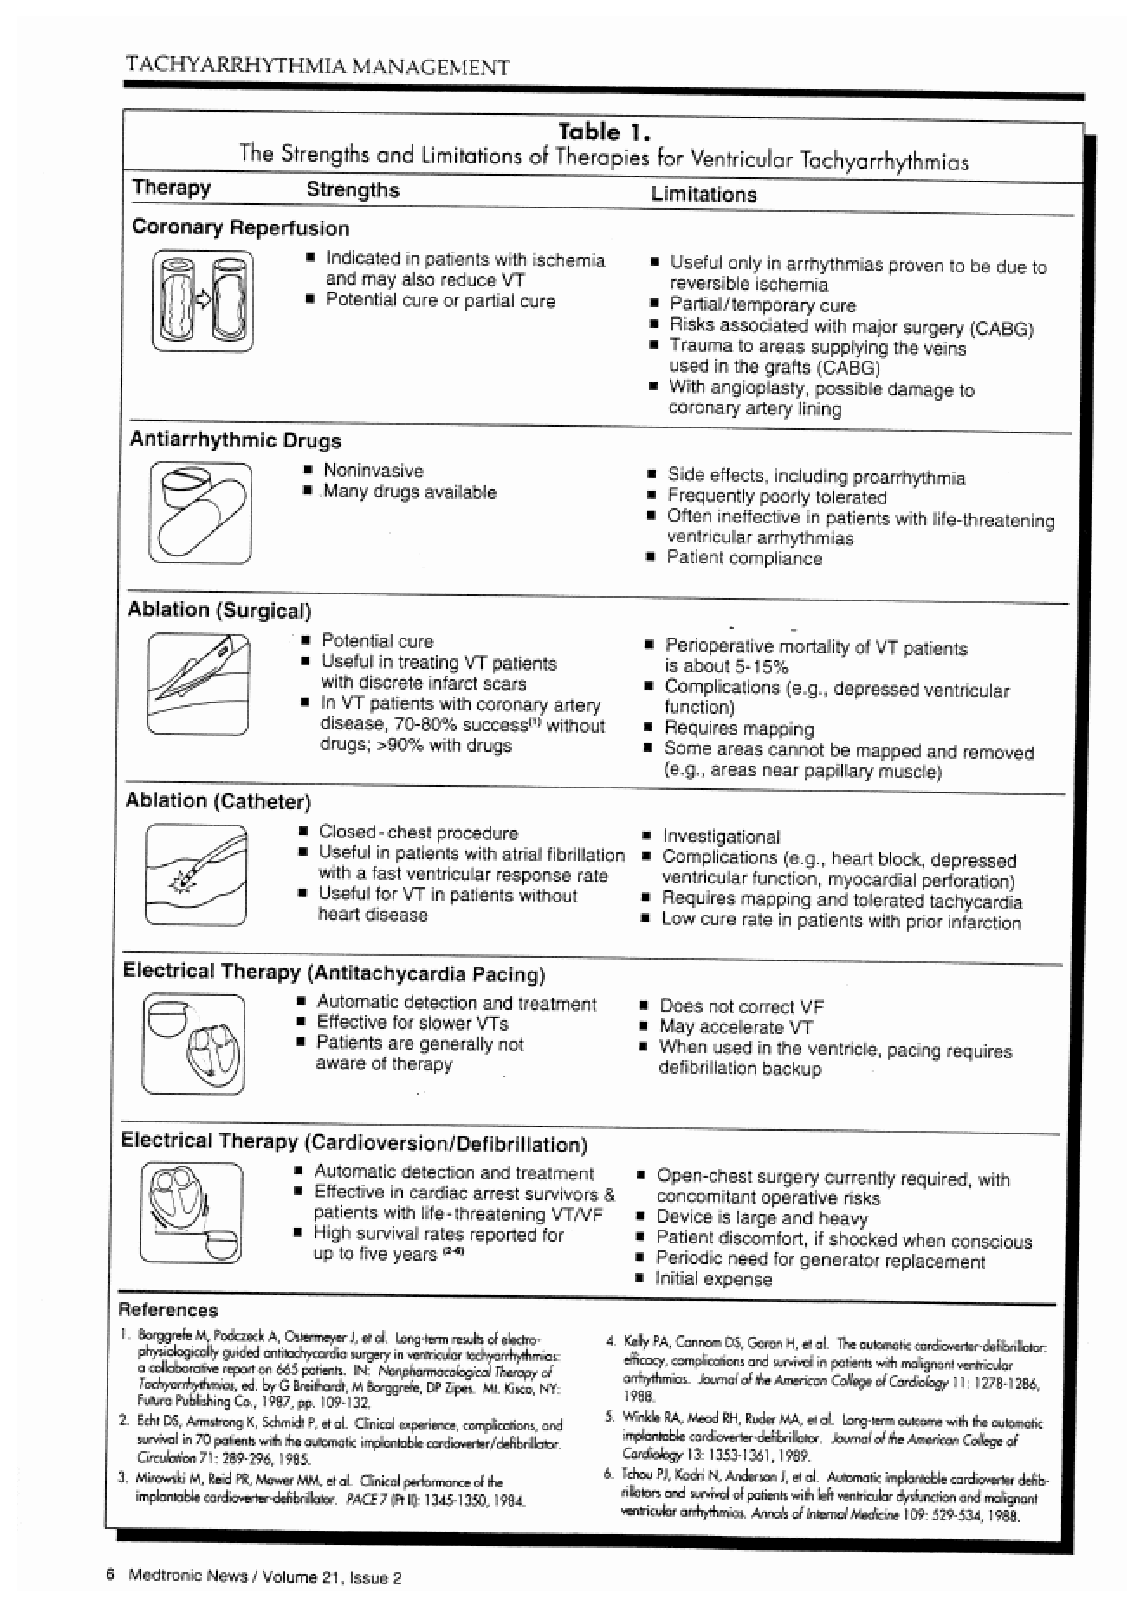
\epsfig{file=electrocardiology/epsfiles/tachy-arryth.eps,width=10cm}
  \caption[Ventricular Tachyarrhythmia Management]{The strenths and
    weakenss associated with the various Ventricular Tachyarrhythmia
    management options}
  \label{fig:tachy-arryth}
\end{figure}

\section{Usefulness of ECG}

The ECG is used to determine what is happening to the heart (how it is
performing, etc.).  This is an ``inverse'' problem (inverse problems are very
difficult to solve) - i.e. given this set of ECGs, what is the heart doing. (
The `forward' problem would be, given that the heart is doing this (i.e. has a
given electrical activation pattern), what is the corresponding ECG - this
would be far easier to solve).

The `inverse' problem is solved largely by pattern recognition.  There are
books of ECGs which illustrate different problems - just find the right ECG
(durations of different waves, heights, etc. give clues to possible
irregularities).There is a standard set of steps to reading an ECG \figref{fig:ecg-interpretation}.

\begin{figure}[htbp] \centering
  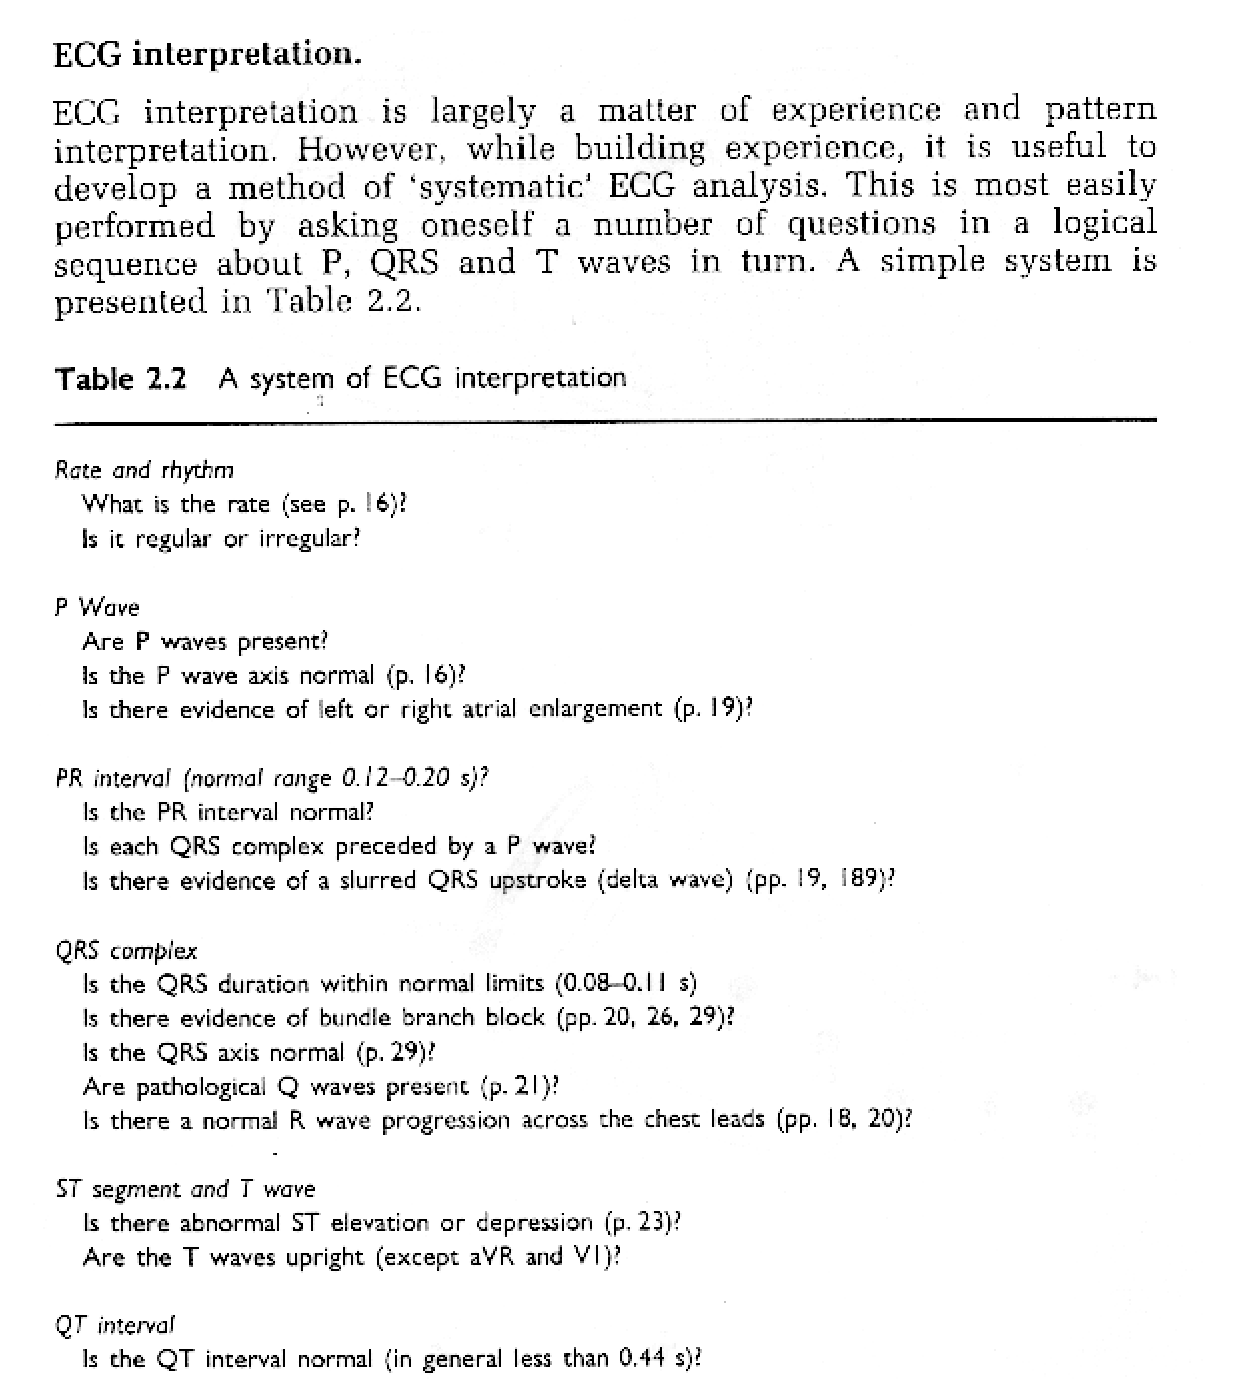
\epsfig{file=electrocardiology/epsfiles/ecg-interpretation.eps,width=10cm}
  \caption[ECG Interpretation]{A procedure for interpreting ECGs}
  \label{fig:ecg-interpretation}
\end{figure}

In later sections we will consider the underlying mathematical theory behind
the ECG.  We now discuss a more generalised approach to ECG monitoring -
namely body surface potential mapping.

\section{Body Surface Potential Mapping (BSPM)}
ECGs do well, but do not provide the whole answer. e.g. they can tell WPW is
present, but not where the accessory pathway is; they can (sometimes) detect
infarcts and ischaemic regions, but not identify where these regions are. A
famous example is the case of Sir Richard Hadlee \figref{fig:hadley} 
who had open chest surgery to
correct is WPW problem (which was identified with an ECG but could not be
localised without more detailed mapping).

\begin{figure}[htbp] \centering
  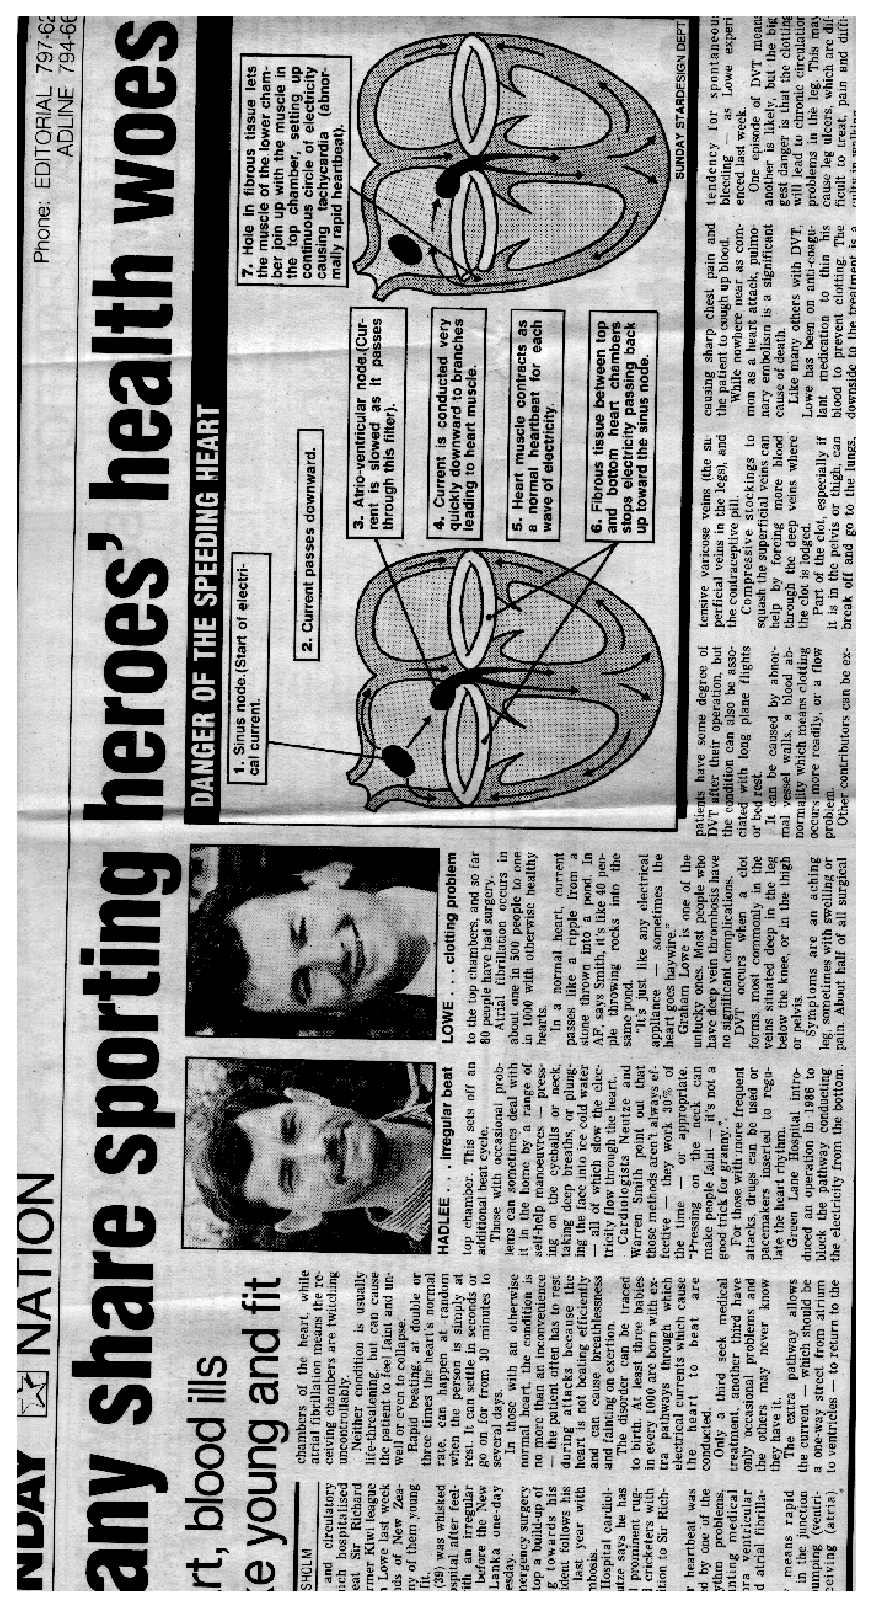
\epsfig{file=electrocardiology/epsfiles/hadley.eps,width=10cm}
  \caption[Sir Richard Hadlee]{The newspaper article
    mentioning Sir Richard Hadlee's WPW problem}
  \label{fig:hadley}
\end{figure}

BSPM was brought about by the development of full chest lead systems
to sample electrical activity at a relatively large number of sites. It began
in the early 60s (?) and is not usually used clinically, however, those places
that use it get good results.  The problems with BSPM are that
it can be more time consuming, there are no standard lead sets, it requires more
setup time (there is a need to store and view a great deal of data), and an
ECG provides a lot of information available on BSPM, suggesting that the extra
work is not worth the effort. 

Two examples of BSPM systems are given in \figref{fig:body-suit2}, 
\figref{fig:body-suit},  \figref{fig:body-suit-utah} and 
\figref{fig:body-suit2-utah}. \figref{fig:body-suit2} and  
\figref{fig:body-suit} are of the system used in Hobart, Australia and contain a large
number of active (dry) electrodes that are embedded between 2 layers of
neoprene. This suit can be applied quickly and a recording obtained in about
the same time as that needed for a standard 12 lead ECG.  The person
standing in \figref{fig:body-suit2} often uses this system in acute patients
(in the ER room for instance) in preference to a 12 lead ECG.  The other 2
figures, \figref{fig:body-suit-utah} and  
\figref{fig:body-suit2-utah} are from a system in use in Salt Lake City, Utah.
Strips of electrodes are placed over part of the torso at pre-specified
locations. Each electrode is full with a conducting gel and contains a
surround of adhesive, so they stick to the skin.  This 32 lead system was
obtain  from looking at maps recorded with 120
leads and doing a statistical decomposition and evalue analysis.  It was found
that an ECG provides approximately 90\% of the information available and 32
leads yield approximately 98\%.

\begin{figure}[htbp] \centering
  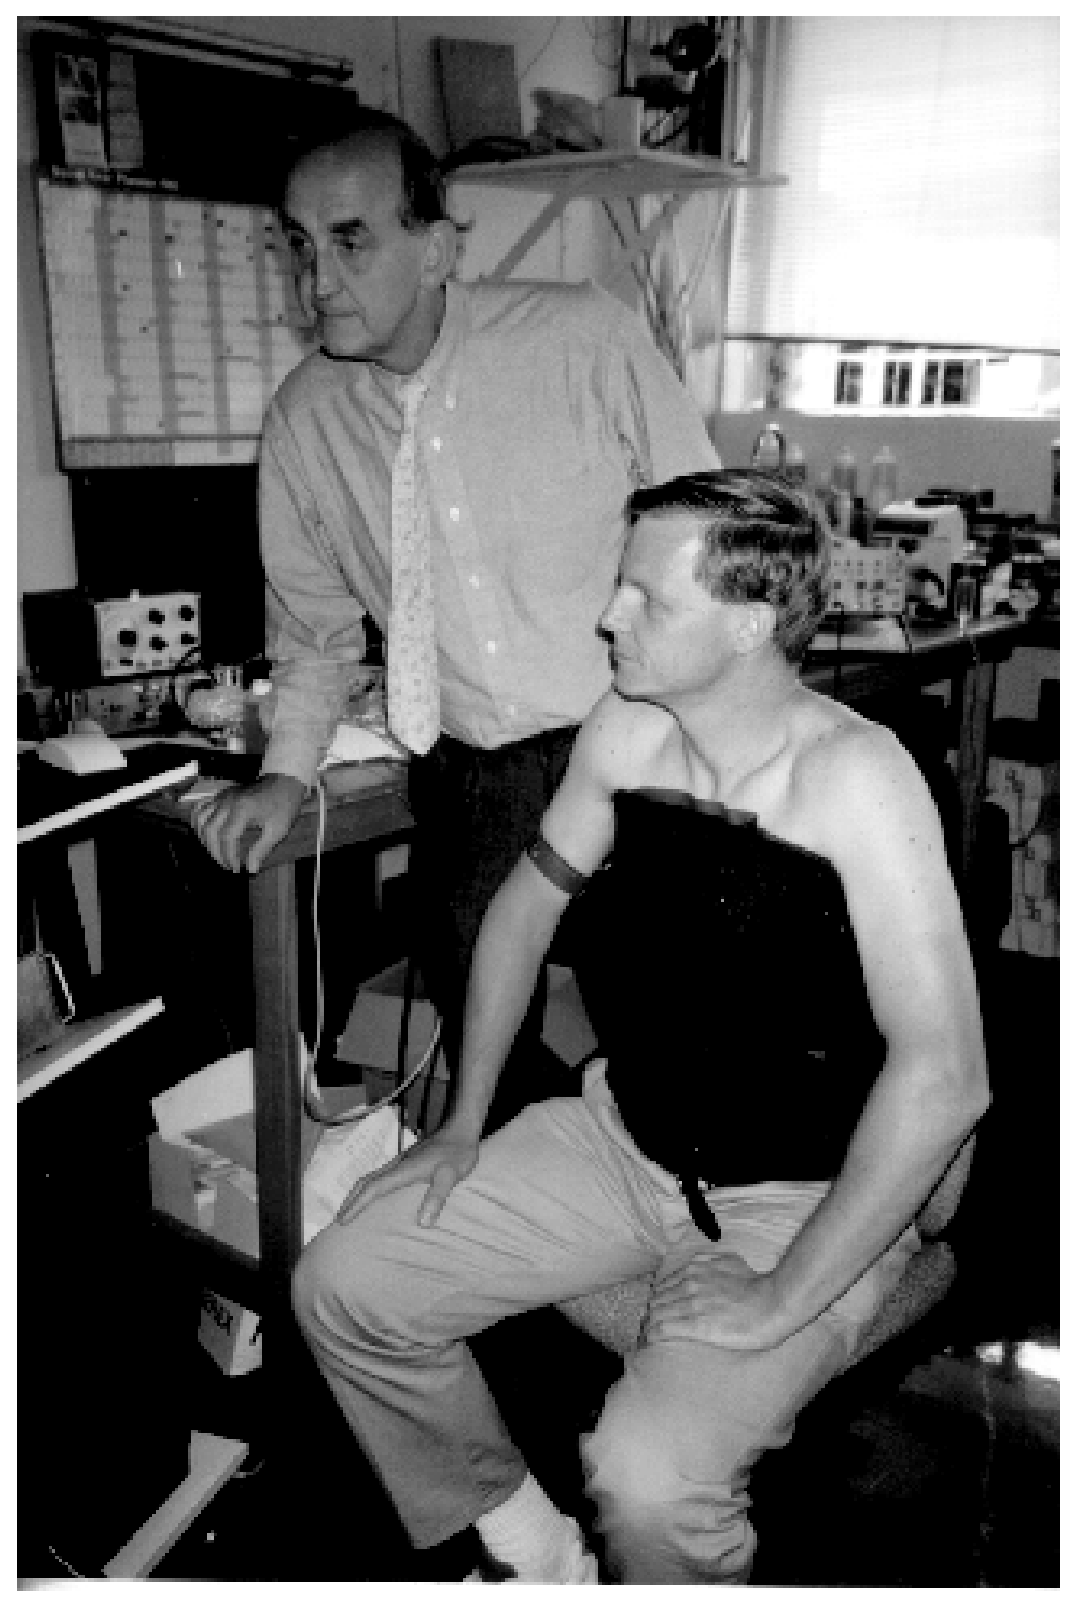
\epsfig{file=electrocardiology/epsfiles/body-suit2.eps,width=10cm}
  \caption[Hobart body surface mapping system]{Hobart Body surface mapping system}
  \label{fig:body-suit2}
\end{figure}

\begin{figure}[htbp] \centering
  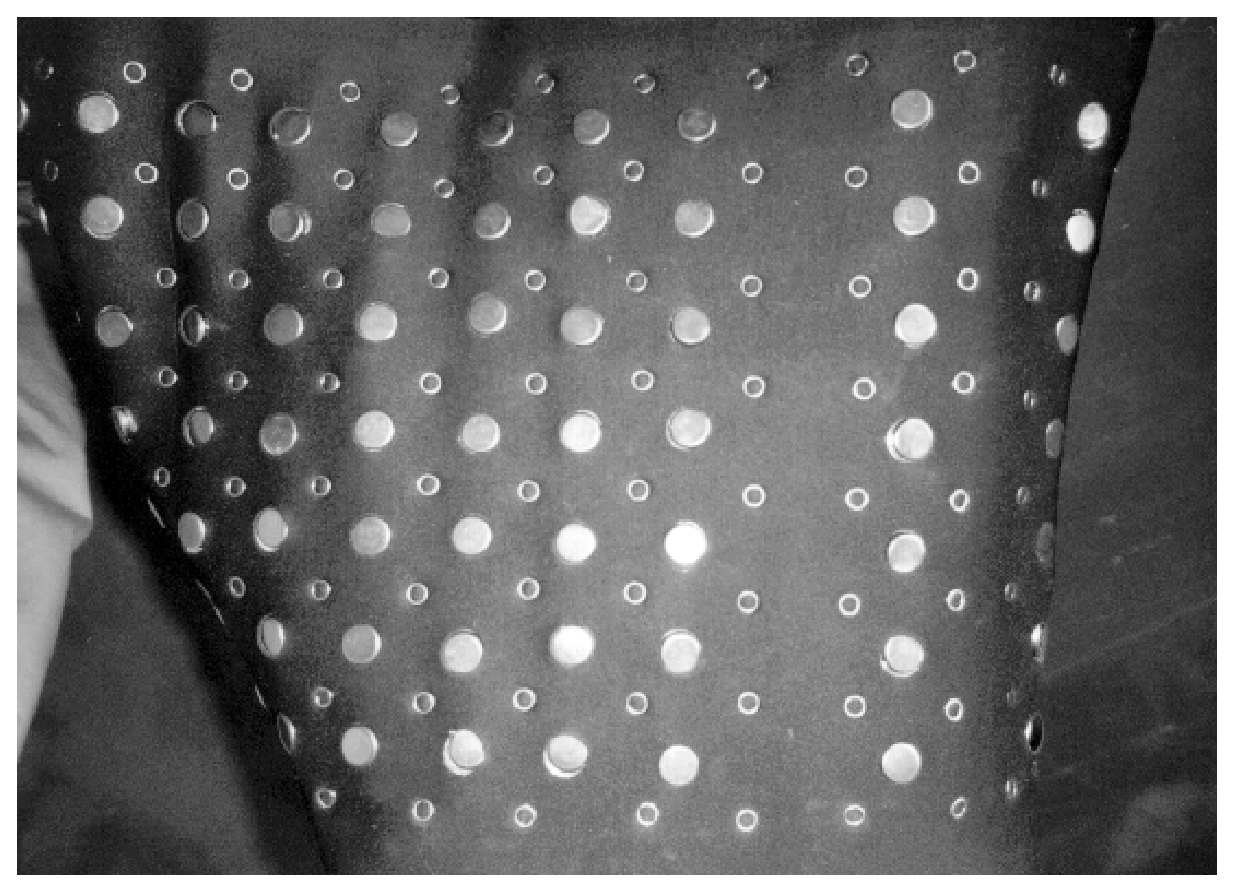
\epsfig{file=electrocardiology/epsfiles/body-suit.eps,width=10cm}
  \caption[Hobart body surface suit]{Hobart Body surface suit}
  \label{fig:body-suit}
\end{figure}

\begin{figure}[htbp] \centering
  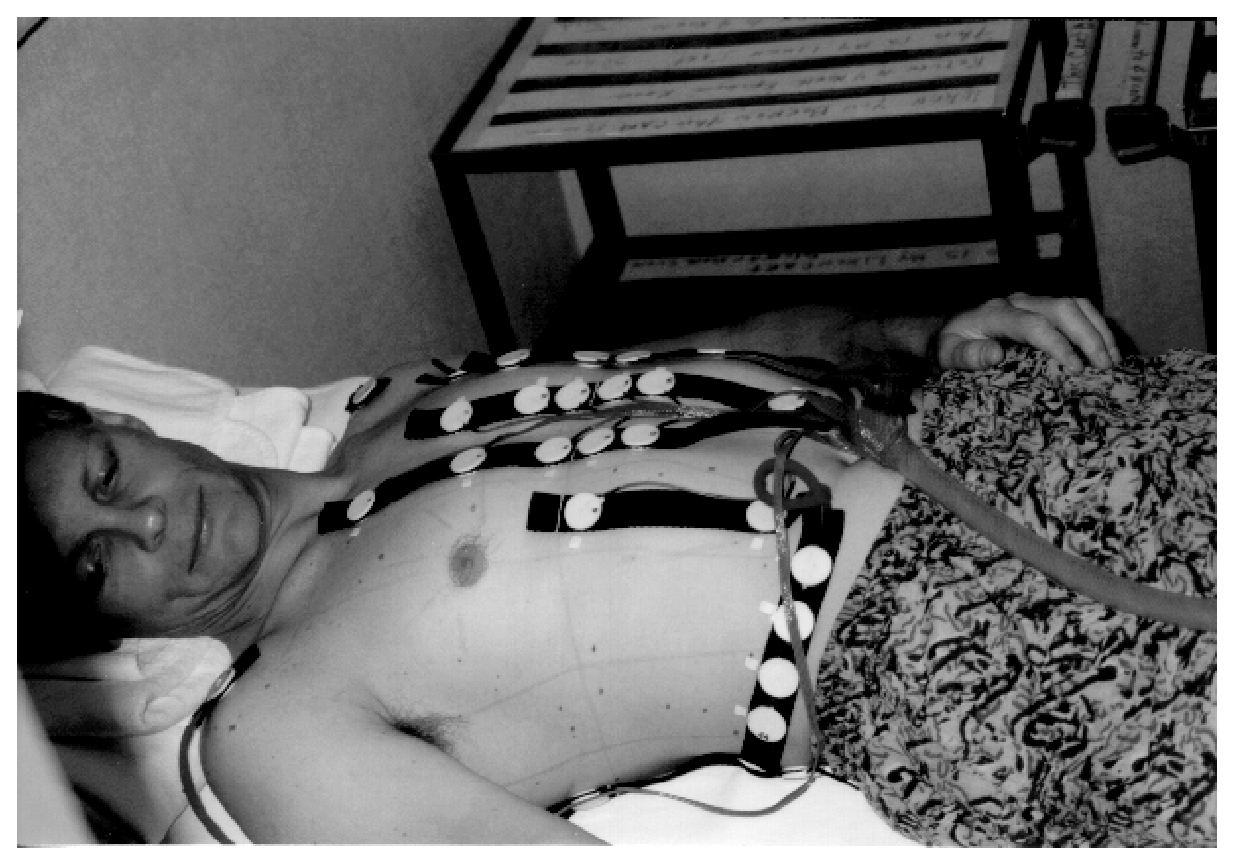
\epsfig{file=electrocardiology/epsfiles/body-suit-utah.eps,width=10cm}
  \caption[Utah body surface mapping suit]{Utah body surface mapping suit}
  \label{fig:body-suit-utah}
\end{figure}

\begin{figure}[htbp] \centering
  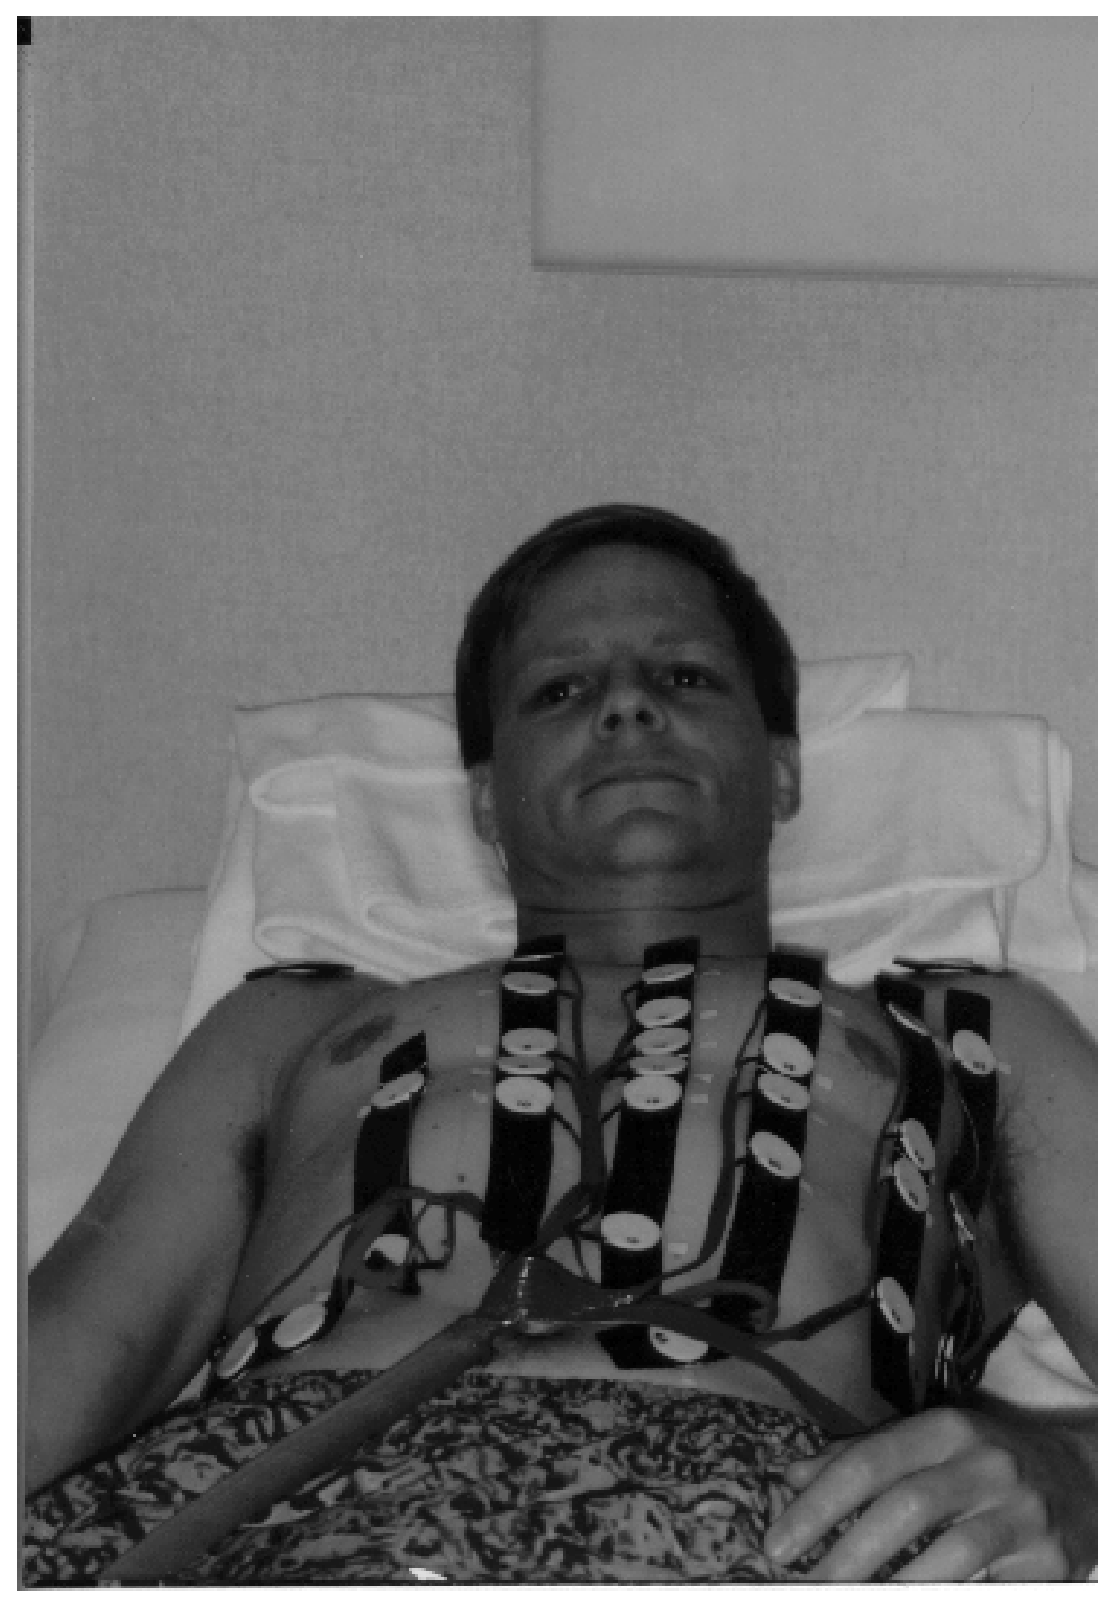
\epsfig{file=electrocardiology/epsfiles/body-suit2-utah.eps,width=10cm}
  \caption[Utah body surface mapping suit - another view]{Utah body surface
    mapping suit- another view}
  \label{fig:body-suit2-utah}
\end{figure}

Schematics of other lead systems are given in \figref{fig:vcg-bspm} and
\figref{fig:bspm-leads}. The first of these shows the location of the standard
ECG leads in a uniform electrode array.  The other figure shows 2 lead sets
that have been proposed which are said to yield almost all the information of
the uniform array. 

\begin{figure}[htbp] \centering
  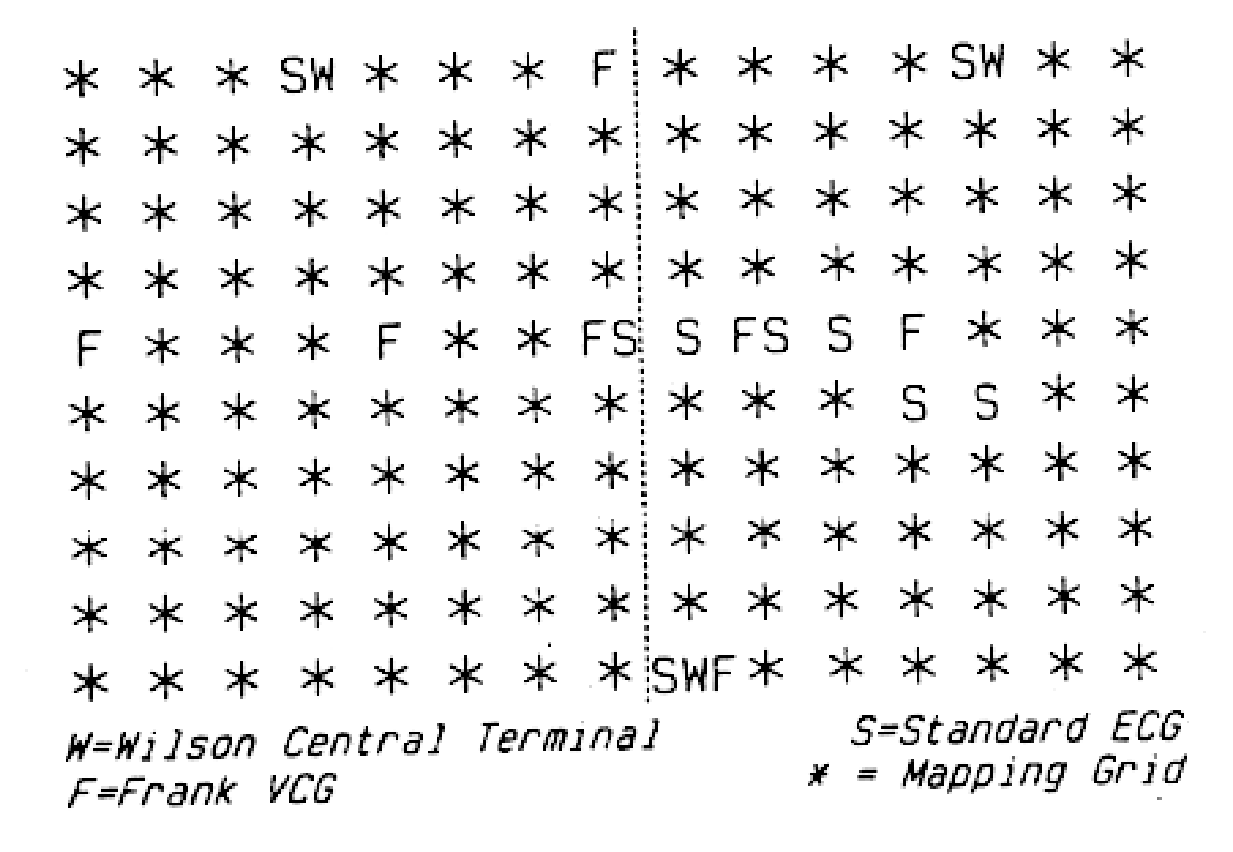
\epsfig{file=electrocardiology/epsfiles/vcg-bspm.eps,width=10cm}
  \caption[Schematic of uniform lead set]{Comparison of torso electrode
    locations for vectorcardiography (F), for standard electrocardiography (S)
    and for body surface potential mapping.  The vertical lines marks the
    sternum.}
  \label{fig:vcg-bspm}
\end{figure}

\begin{figure}[htbp] \centering
  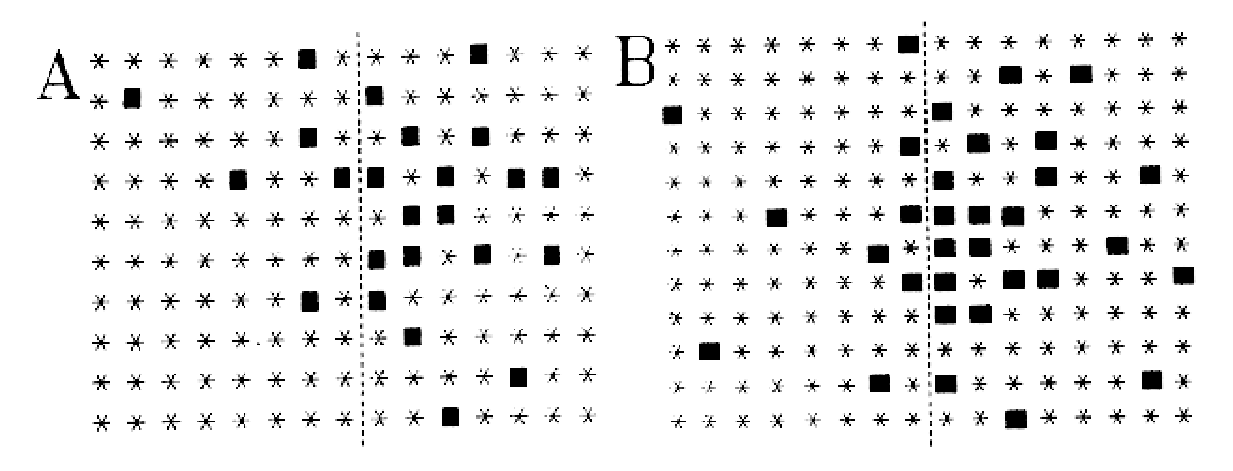
\epsfig{file=electrocardiology/epsfiles/bspm-leads.eps,width=10cm}
  \caption[Various BSPM electrode locations]{Utah body surface
    mapping suit- another view. Electrocardiographics lead sets proposed by Barr
    (A- Duke) and Lux (B- Salt Lake City) }
  \label{fig:bspm-leads}
\end{figure}

Implantable defibrillators are being widely used
instead of fixing the problem. There is a lack of good modelling and diagnostic
cabability. However, it is our view that with good modelling and new imaging techniques, and the
cooperation of clinical staff, a great deal of progress can be made. We
currently have our own BSPM system.

\subsection{BSPM at Halifax, Canada}
We present in this section real BSPM maps recorded from patients suffering
from WPW in Dalhousie University, Halifax, Canada.  
The emphasis on this system is due to the
availability of the measured maps.  As mentioned above, WPW is a condition in
which an accesory pathway exists between the atria and ventricles. Although this does not affect a large proportion of the population it is a
situation in which BSPM has been very successful since the site of the
accessory pathway can, in most cases, be determined before inserting a
catheter for ablation (5-10 years ago open heart surgery was required).
 It is
relatively easy to fix (just cut/ablate the tissue involved) once the region
has been localised.  It is also fairly easy to detect on an ECG
\figref{fig:deltawave-ecg}, \figref{fig:deltawave} but it cannot be localised
using a standard ECG.

\begin{tabular}{lcp{13cm}}
Cause & - & breakdown of ``insulation'' between atria and ventricles.  Ventricles
are being stimulated from above and below - loss of pumping efficiency.\\
Cure & - & find accessory pathway and ablate (i.e. burn part of the tissue with a
catheter - this is inserted in the leg).
\end{tabular}

\begin{figure}[htbp] \centering
  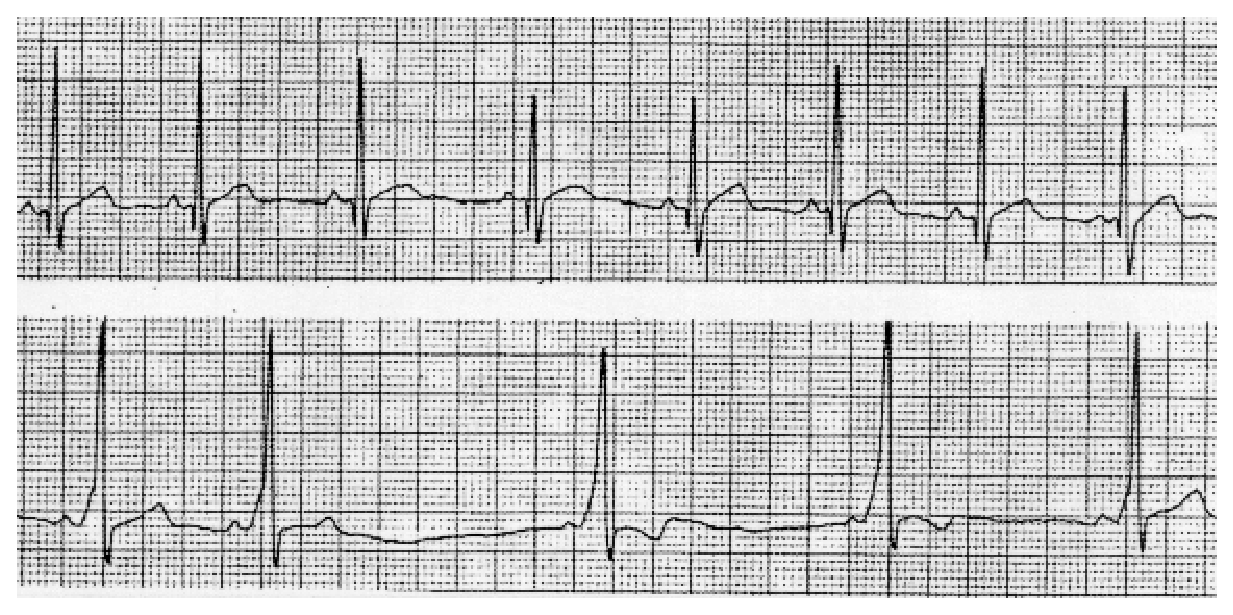
\epsfig{file=electrocardiology/epsfiles/deltawave-ecg.eps,width=10cm}
  \caption[WPW ECG]{Part of an ECG of a WPW condition.  At slower rates
    (bottom) a delta wave is more prominent that it is at higher rates}
  \label{fig:deltawave-ecg}
\end{figure}

 \begin{figure}[htbp] \centering
  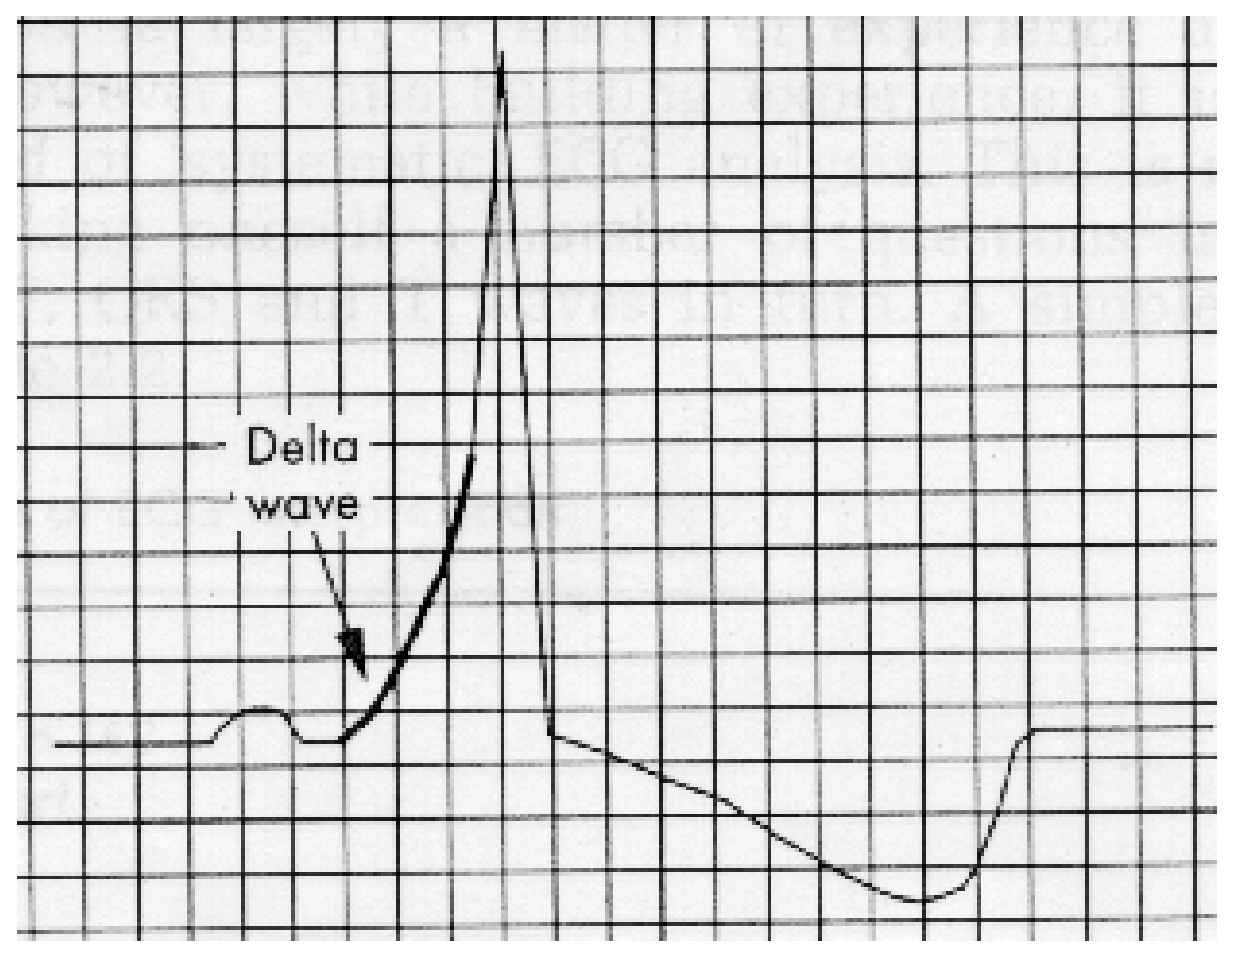
\epsfig{file=electrocardiology/epsfiles/deltawave.eps,width=10cm}
  \caption[Delta wave]{Scehmatic representation of ECG features of the WPW
    patten.}
  \label{fig:deltawave}
\end{figure}

Figure \figref{fig:halifax-mesh} illustrates the electrode locations used in
the Halifax system (black dots - left hand side is the front).  Recordings
from a healthy male are given in \figref{fig:hal-leads-norm-front} (front) and
\figref{fig:hal-leads-norm-back} (back).  Note that some of the leads given no
recording, so are discard in the final analysis.  The position of the standard
V1 and V2 leads are marked.  The recordings given are based on averages of 10
seconds of recordings.

 \begin{figure}[htbp] \centering
  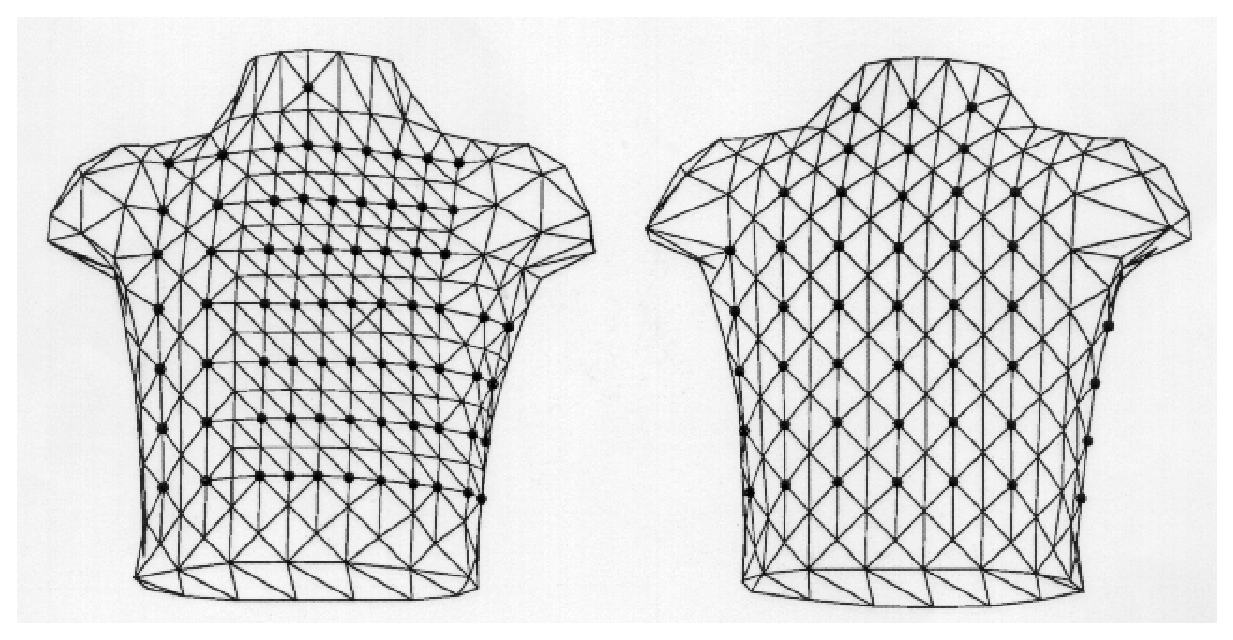
\epsfig{file=electrocardiology/epsfiles/halifax-mesh.eps,width=10cm}
 \caption[Lead location of Halifax BSPM system]{The location of the electrodes
   used in the BSPM system at Halifax.  The left hand side represents the
   front, and electrodes are denoted using black dots}
  \label{fig:halifax-mesh}
\end{figure}

 \begin{figure}[htbp] \centering
  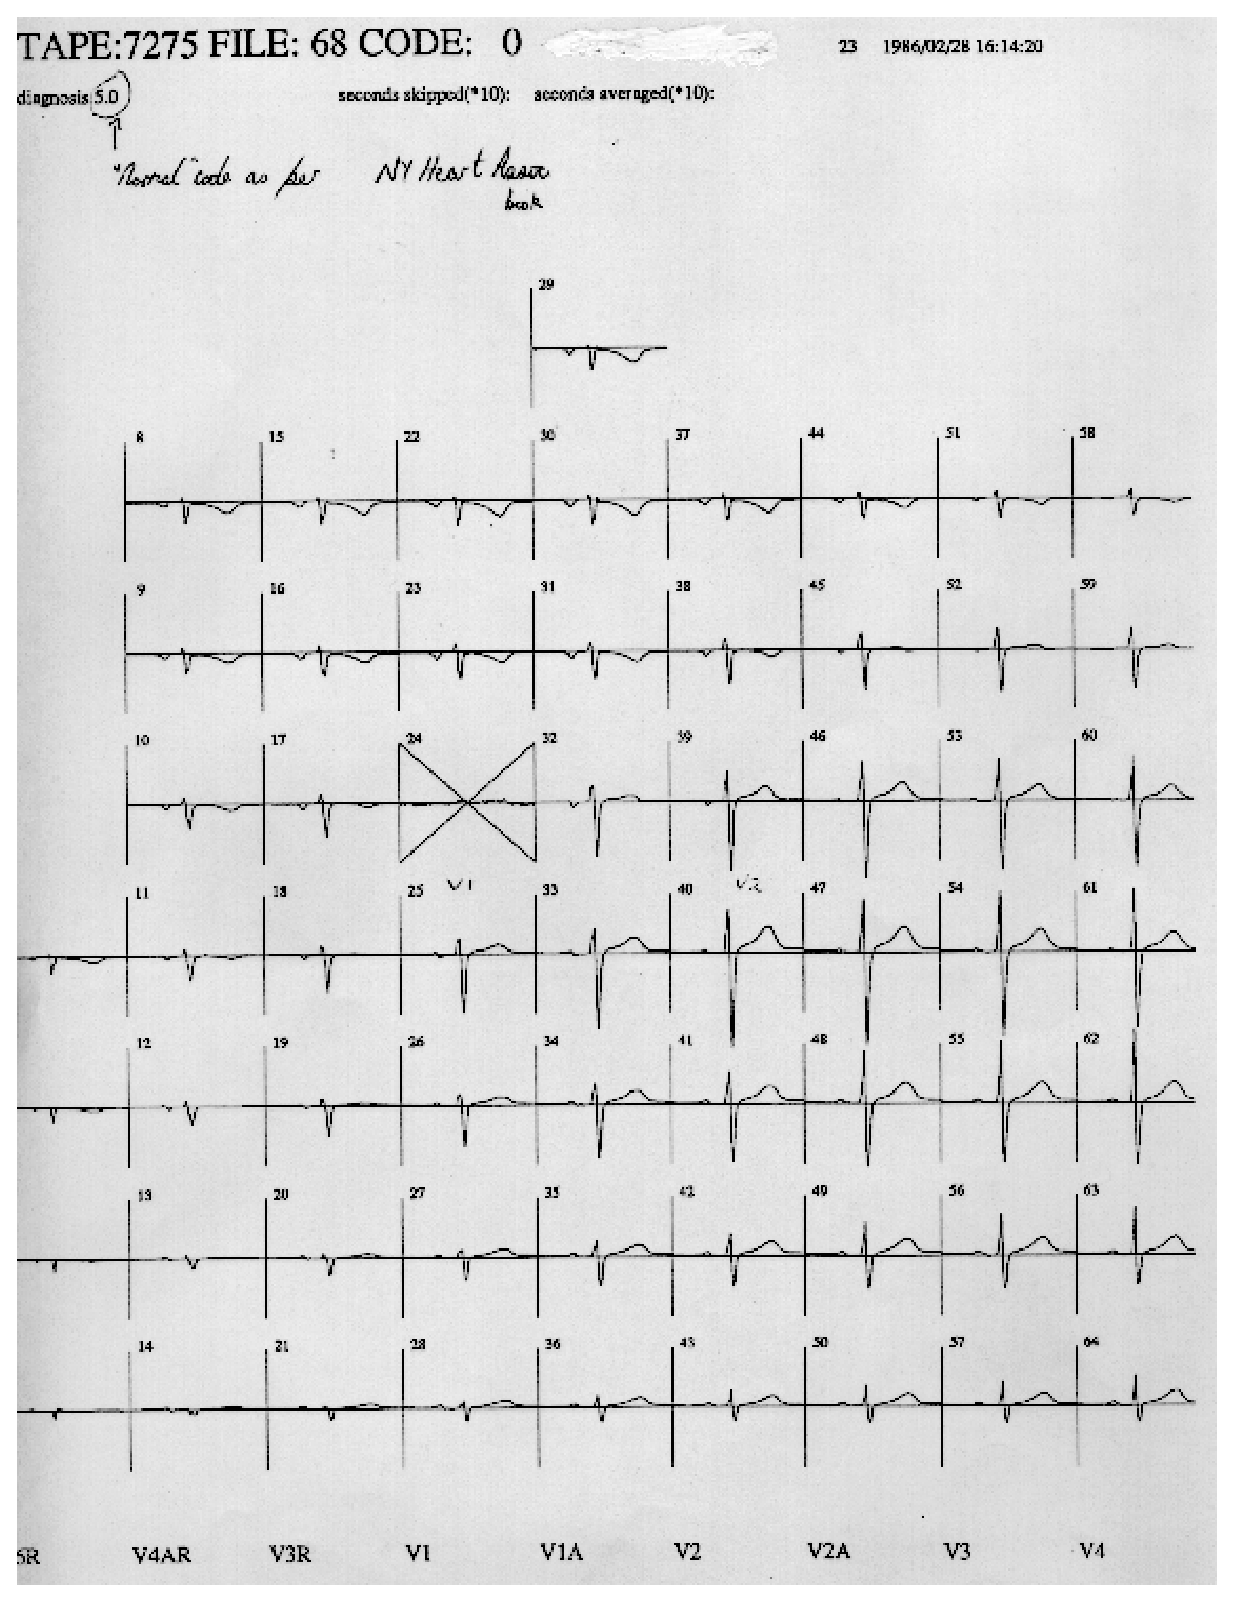
\epsfig{file=electrocardiology/epsfiles/hal-leads-norm-front.eps,width=10cm}
 \caption[Normal BSPM recording]{The front recordings from a normal male 
 using the
   Halifax BSPM system (10 seconds of recordings that have been averaged.  Note that some leads give no recording and are
   therefore discarded from further analysis.  The location of the leads V1
   and V2 have been marked.  The left hand code is the code as per the NY
   Heart Association handbook}
  \label{fig:hal-leads-norm-front}
\end{figure}

 \begin{figure}[htbp] \centering
  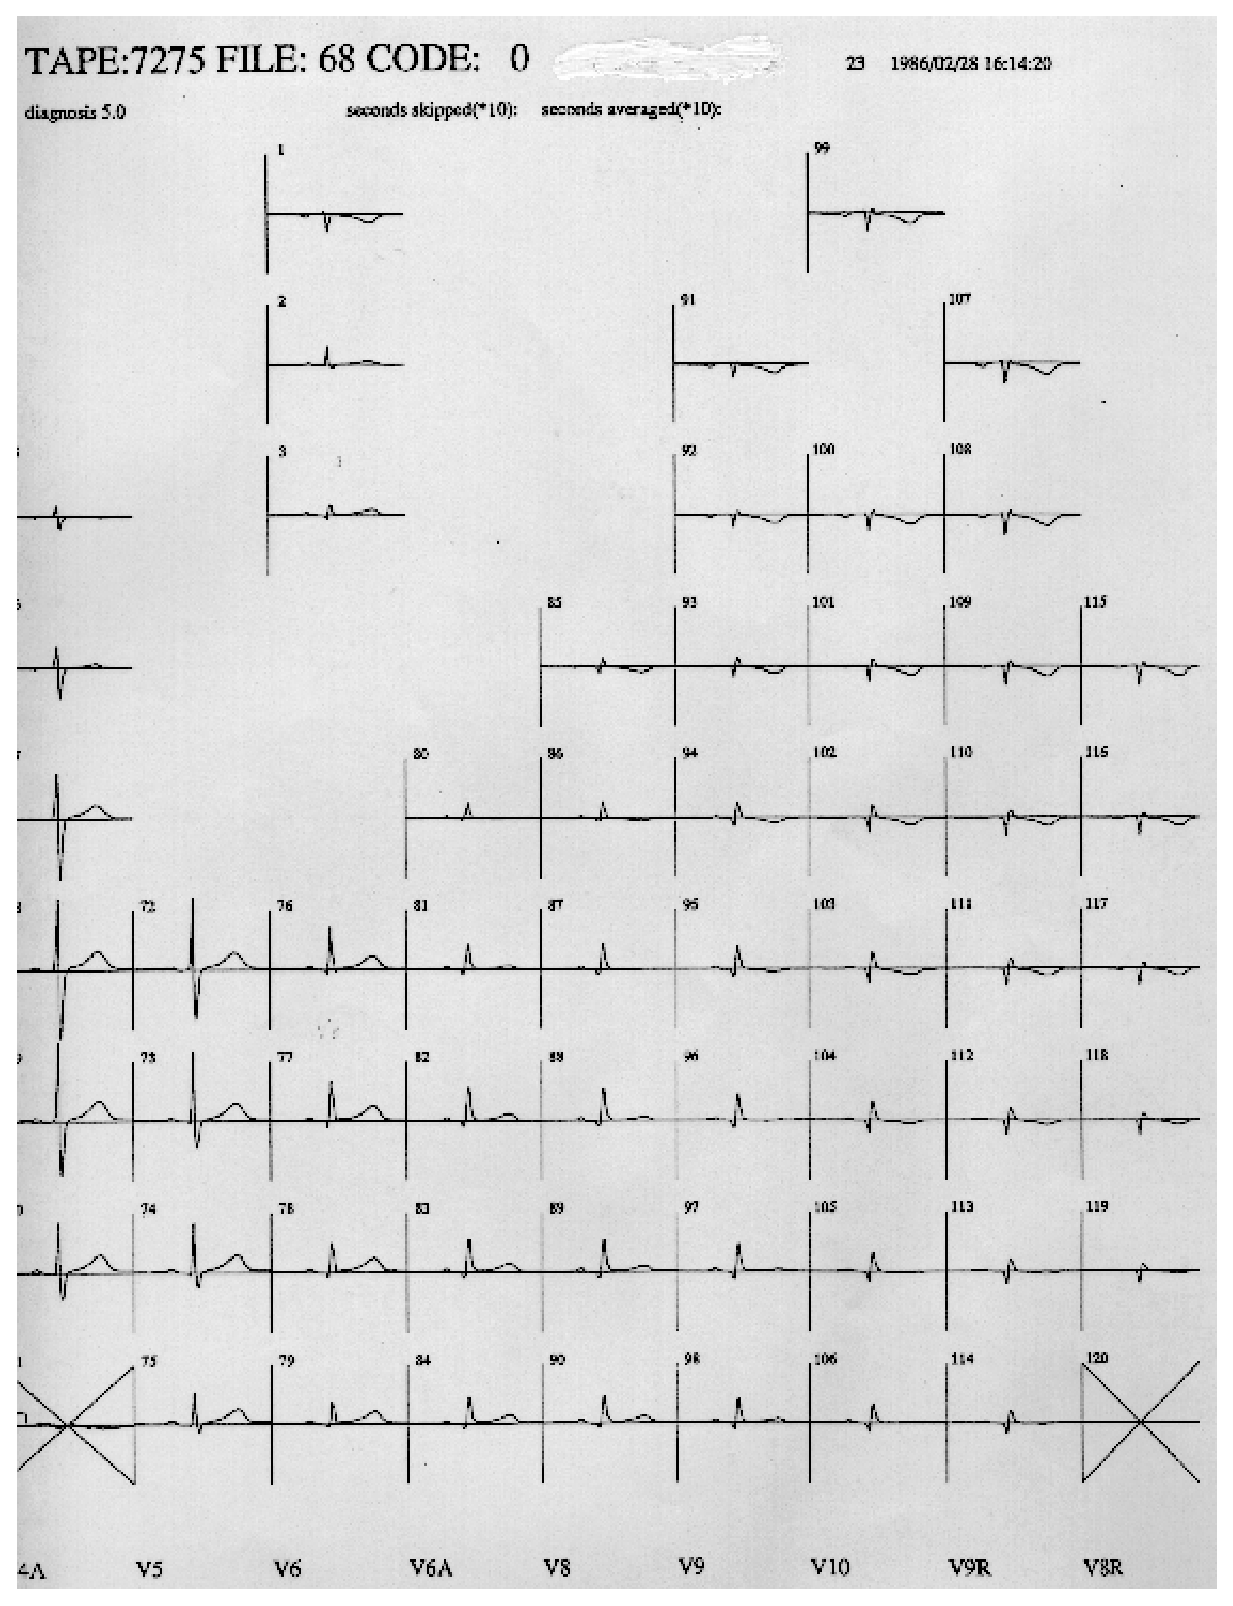
\epsfig{file=electrocardiology/epsfiles/hal-leads-norm-back.eps,width=10cm}
 \caption[Normal BSPM recording - back]{The back recordings from a normal
   male using the Halifax BSPM system }
  \label{fig:hal-leads-norm-back}
\end{figure}

Fiducial markers (start and end of QRS etc) are then obtained by looking at
the Frank VectorCardiograph leads \figref{fig:hal-vcg-normal} (i.e. looking at the difference in potential
across the body, front-back of the body and up/down on the body). 

 \begin{figure}[htbp] \centering
  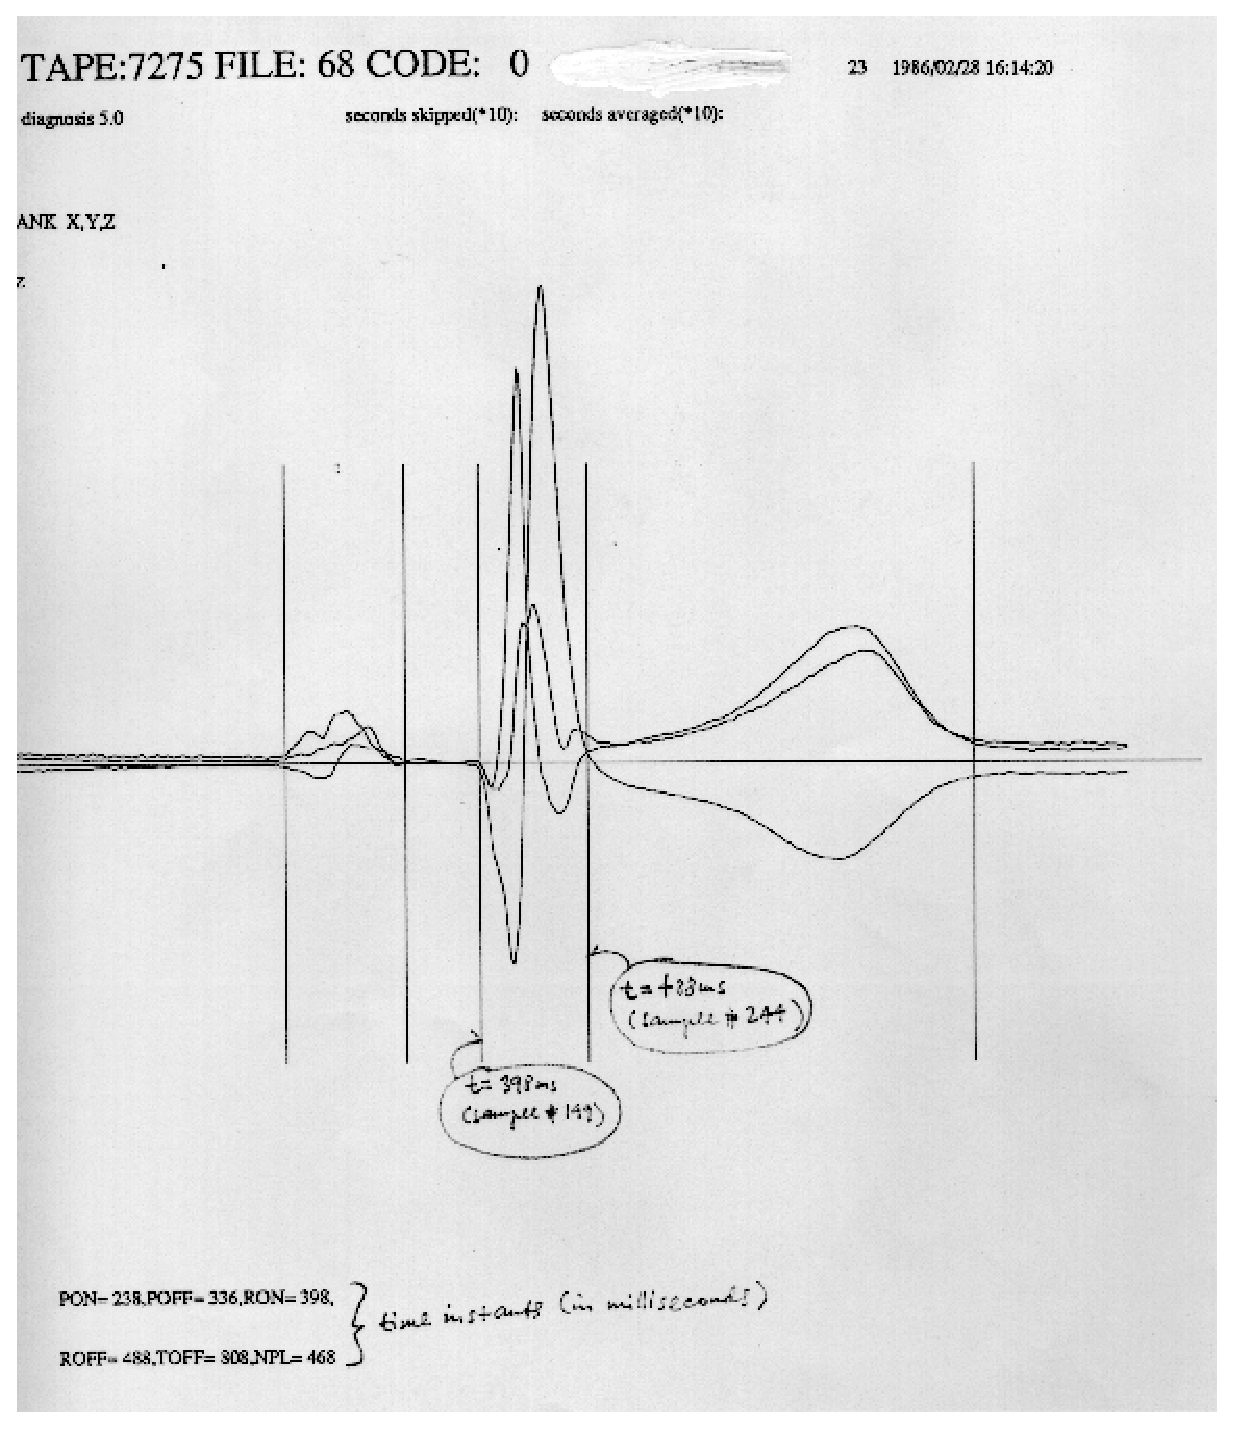
\epsfig{file=electrocardiology/epsfiles/hal-vcg-normal.eps,width=10cm}
 \caption[Normal VCG from Halifax system]{ The VCG used to determine the
   Fiducial markers. PON is the start of the P wave (in ms) POFF the end of
   the P wave, RON and ROFF the equivalent times for the R wave and TOFF is
   end of the T wave. }
  \label{fig:hal-vcg-normal}
\end{figure}

After the fiducial markers have been identified, the data is interpolated to
present the body surface potential maps seen in
\figref{fig:hal-bspm-normala} to \figref{fig:hal-bspm-normalc}. These figures
are maps of the contours of potential at 10 ms intervals.  The first maps are
simply just noise (since these are before activation) and the times
corresponding to the fiducial markers (RON and ROFF) are identified. RPK
corresonds to the peak of the QRS.  The location of the extrema are also
plotted and negative potentials are given in dashed contour lines. 

 \begin{figure}[htbp] \centering
  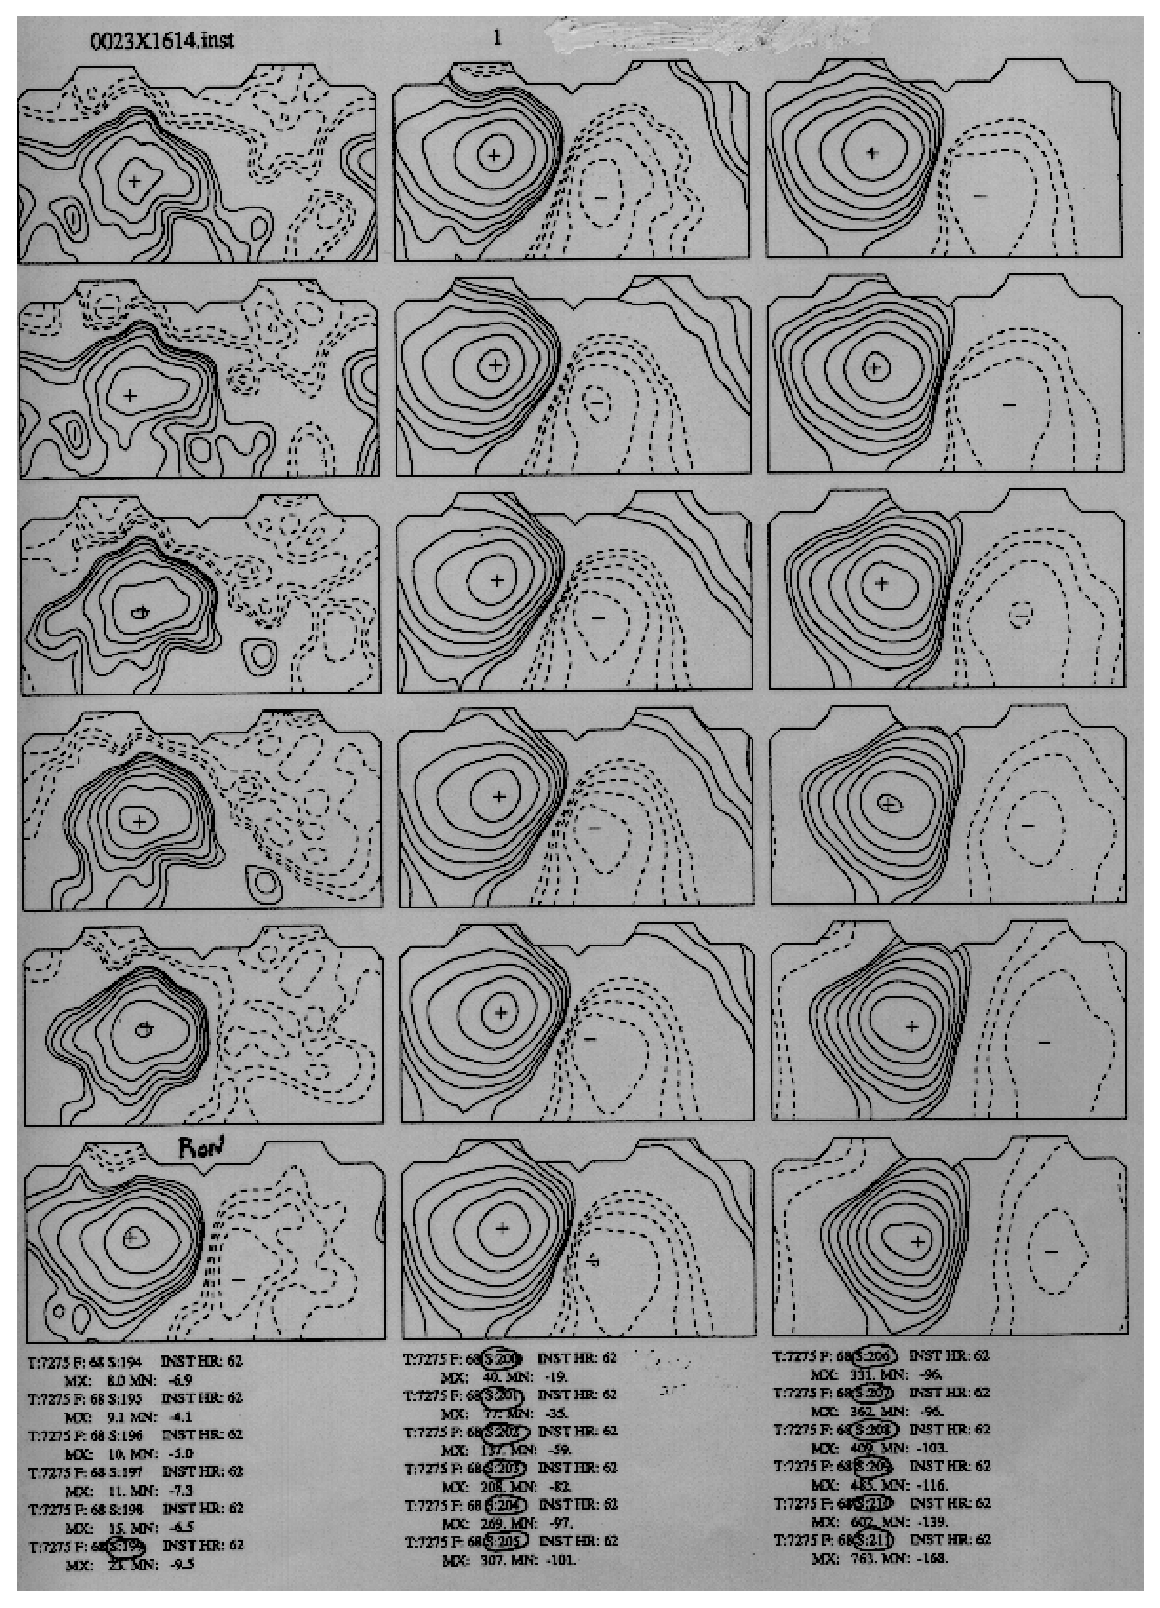
\epsfig{file=electrocardiology/epsfiles/hal-bspm-normala.eps,width=10cm}
 \caption[Normal BSPM maps (a)]{Isopotential lines for a normal patient at
 10 ms intervals.  The first maps are
simply just noise since these are before activation and the times
corresponding to the fiducial markers RON and ROFF are identified. RPK
corresonds to the peak of the QRS.  The location of the extrema are also
plotted and negative potentials are given in dashed contour lines.}
  \label{fig:hal-bspm-normala}
\end{figure}

\begin{figure}[htbp] \centering
  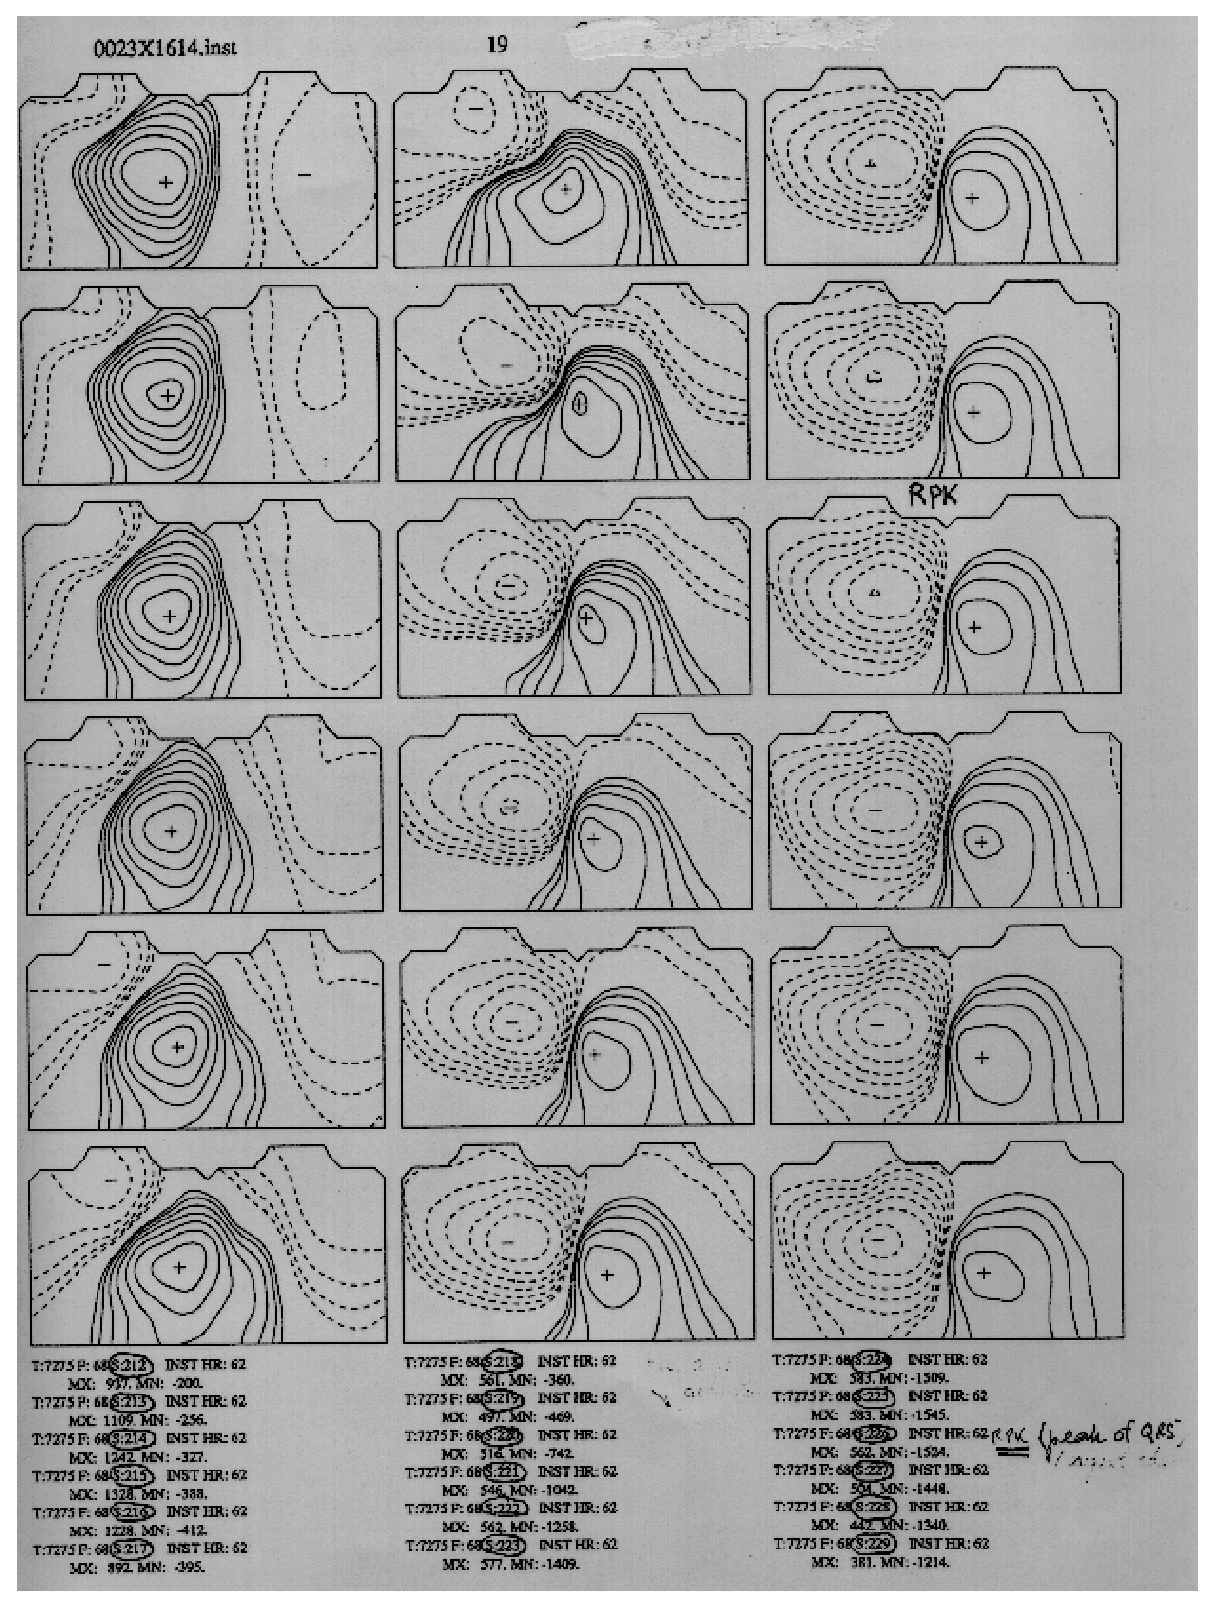
\epsfig{file=electrocardiology/epsfiles/hal-bspm-normalb.eps,width=10cm}
 \caption[Normal BSPM maps (b)]{Normal BSPM maps (b) }
  \label{fig:hal-bspm-normalb}
\end{figure}

\begin{figure}[htbp] \centering
  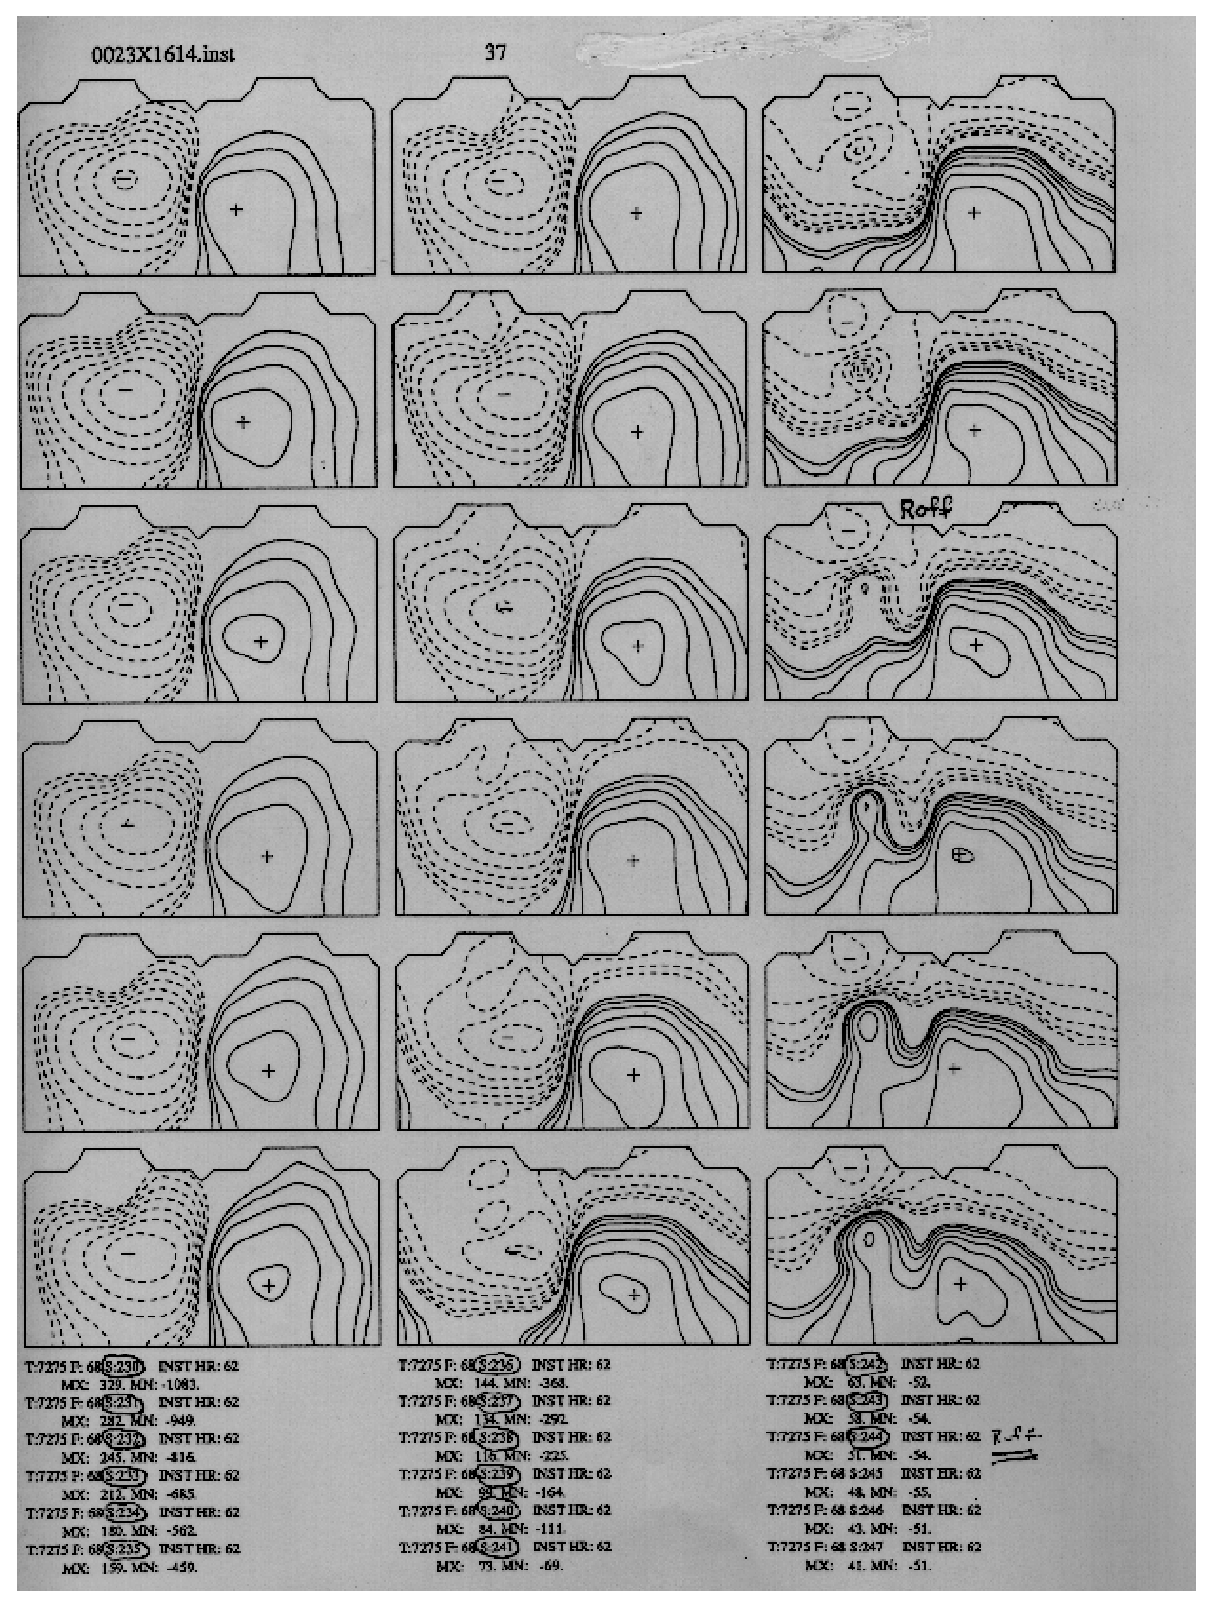
\epsfig{file=electrocardiology/epsfiles/hal-bspm-normalc.eps,width=10cm}
 \caption[Normal BSPM maps (c)]{Normal BSPM maps (c) }
  \label{fig:hal-bspm-normalc}
\end{figure}


\subsubsection{Things to look for}
-positions of maximum and minimum and how these move (and locations of
``zero'' line).
 
\begin{tabular}{lcl}
-before RONN  & - & noise\\
-early R & - & septal activation
\end{tabular}

As activation reaches the apex, the negative region moves over the right
shoulder.

As activation moves up (``deflection'' pointing outward?) there is widespread
left ventricular and right ventricular epicardial breakthrough.  The pattern
can become complicated and variable.  Usually the maximum moves slowly around
the back \figref{fig:bspm-max-min}.

\begin{figure}[htbp] \centering
  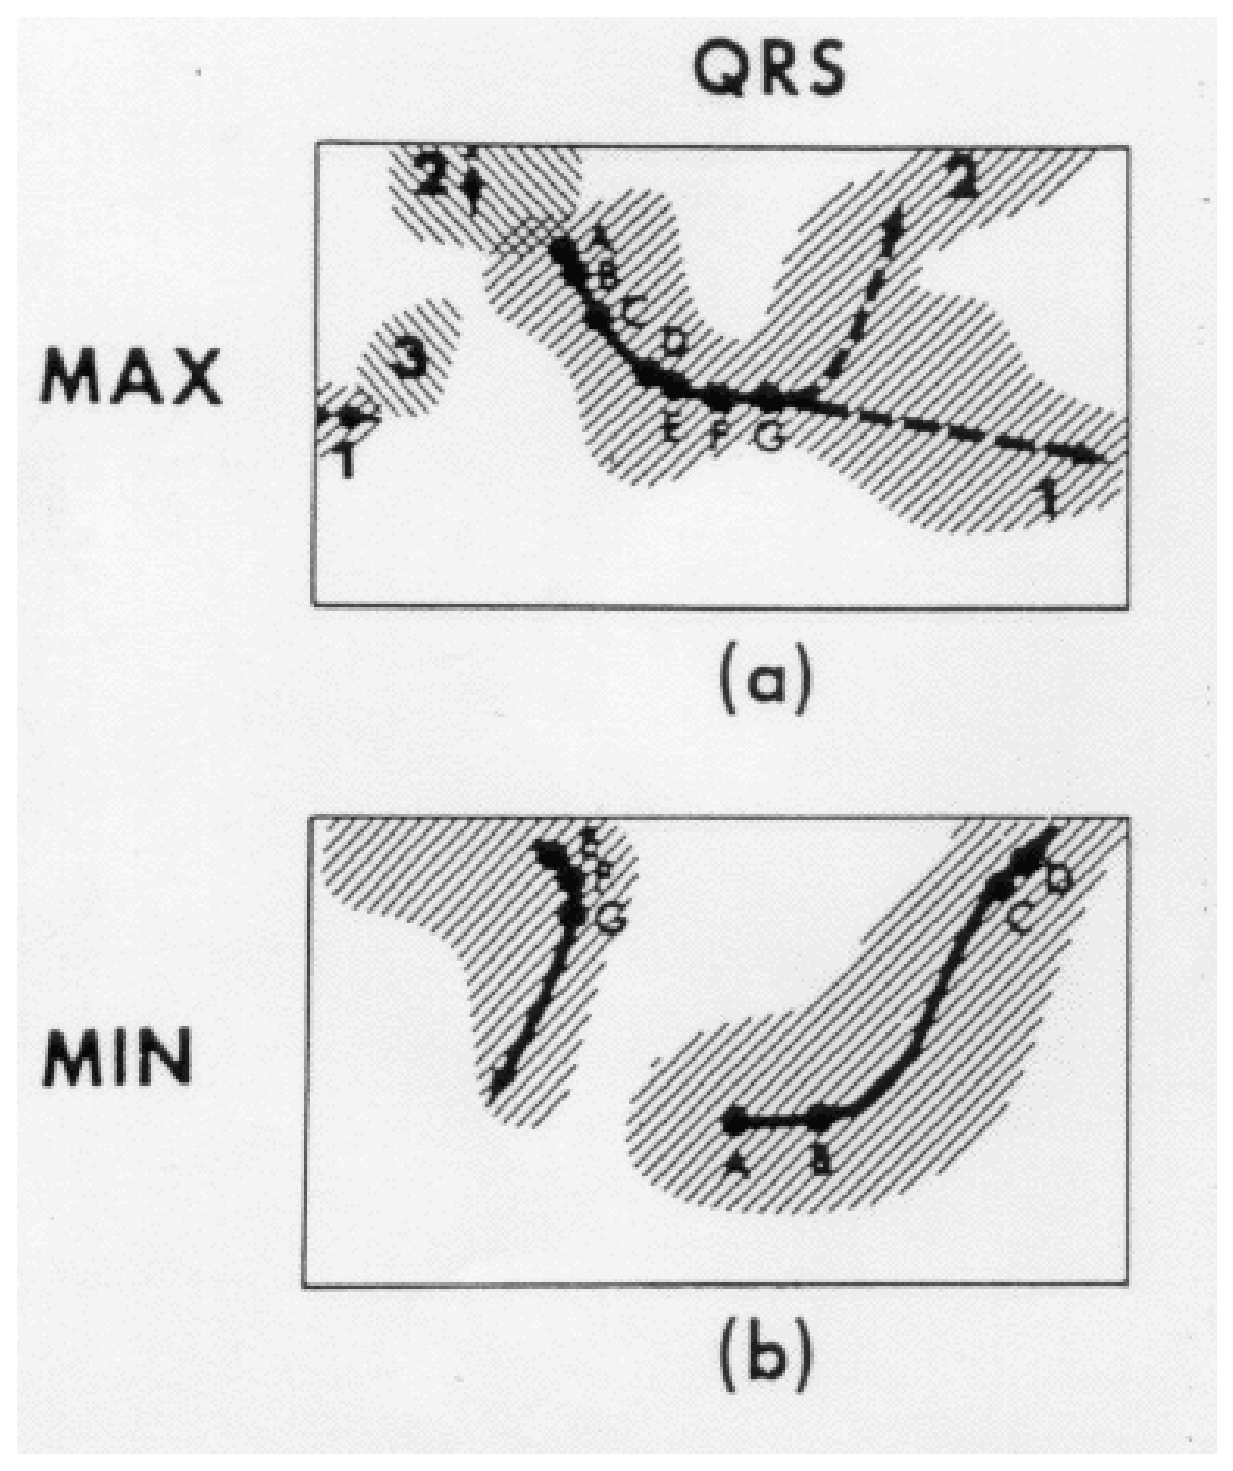
\epsfig{file=electrocardiology/epsfiles/bspm-max-min.eps,width=10cm}
  \caption[BSPM max-min trajectories]{Trajectory maps depicting postion of the
    maxima (top) and minima (bottom) during the QRS copmlex.  The left half of
    each map represents the front of the torso.  Selected instants, labelled
    A through G, are shown.  During the end of the QRS complex, three
    variations (1, 2, and 3) are observed}
  \label{fig:bspm-max-min}
\end{figure}


\subsection{Abnormal Maps}
To help in the interpretion of BSPM from WPW patients, Dalhousie University
 has a model of a human heart (anatomically accurate) in a
model of a torso.  It had a rule-based activation process (cellular-automata,
cells 1mm$^{3}$), and each cell had a set of rules about when it will become
activated and for how long.   This determines epicardial potentials and then
a BEM torso model was used to solve for torso potentials (homogenous torso).

They ran a number of simulations for a number of pre-excitation slices (\figref{fig:hal-heart-model}) and calculated the body surface potentials for each preexcitation
(most prominent differences).  The results of each of these simulations are 
shown in \figref{fig:hal-bspm-template}. The locations
  of the extrema and respective regions of positivity and negativity are used
  to distinguish each map.  These templates are used to help localise the
  accesory pathway.  A patient suffering from WPW (diagnosed from a standard
 ECG) will have a body surface map taken.  This is then compared to the
 templates and the accessory pathway site estimated.  The patient will then
 undergo catheter surgery to localise the  site (starting at the estimated
 site).  In almost all cases, the estimated site corresponds to the site that
 is ablated.  Examples of real maps, and the actual ablation site
 are given in \figref{fig:hal-bspm-wpw1} to  
\figref{fig:hal-bspm-wpw6}.  Note how well these sites are predicted using
  the templates. 

\begin{figure}[htbp] \centering
  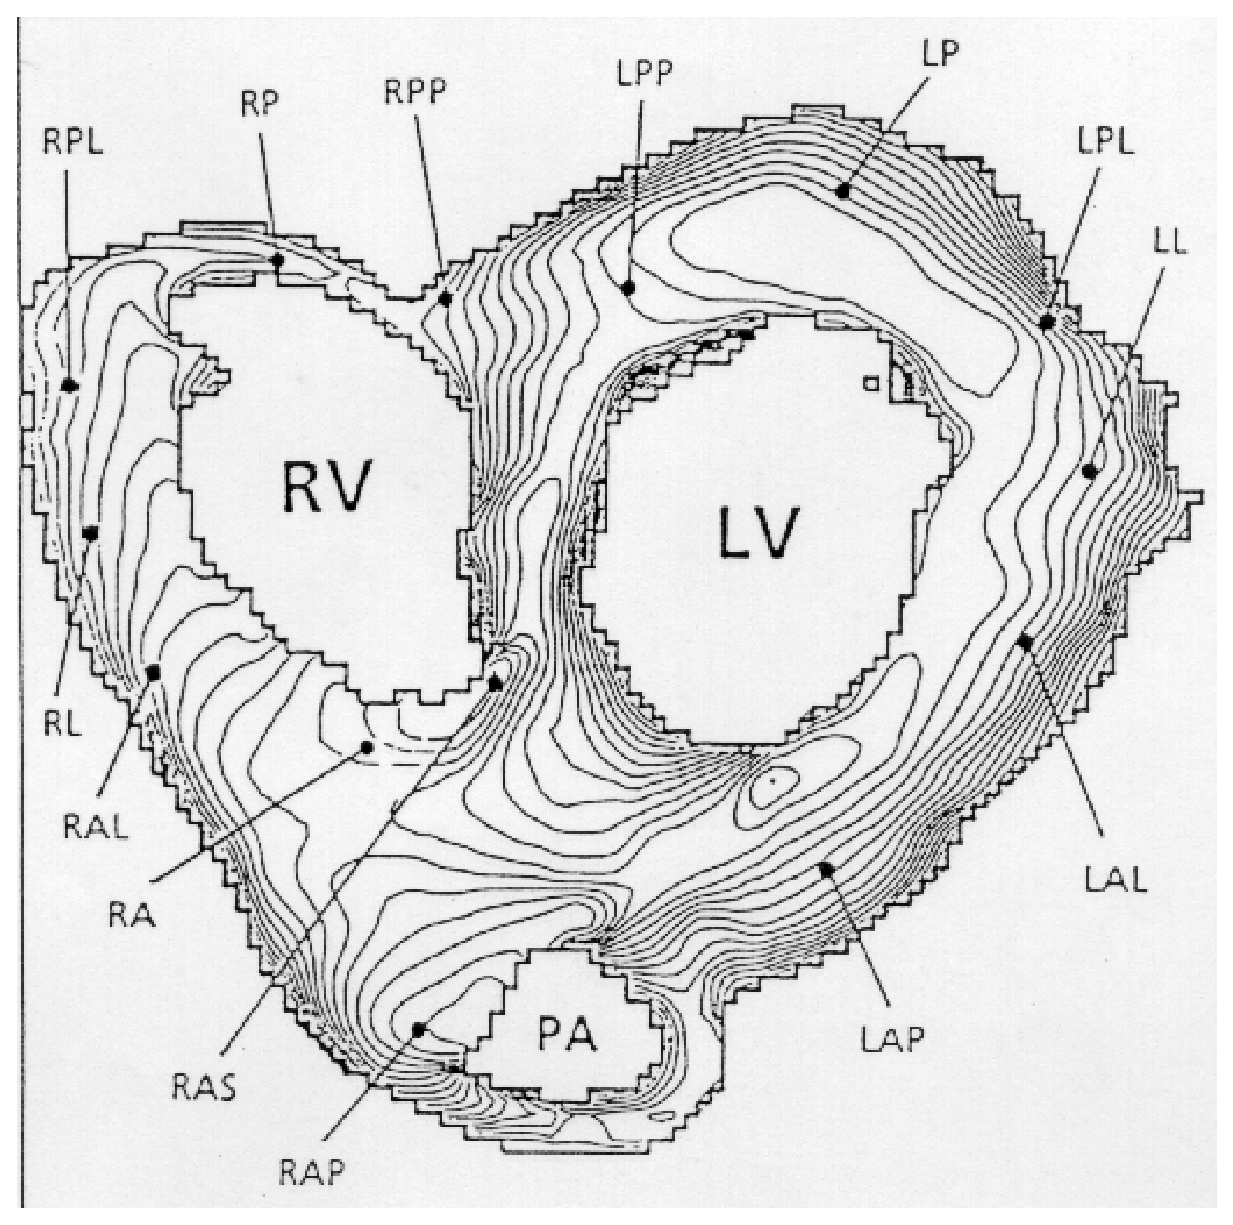
\epsfig{file=electrocardiology/epsfiles/hal-heart-model.eps,width=10cm}
  \caption[Halifax Heart Model]{Top 20 Bassal sections of the ventricular
    haeart model used at Halifax.  There were 14 preexcitation sites.  The
    sections, which are 1 mm apart, are represented by smoothed contour lines
    to achieve a better rendering of the shape.  Note that the ventricular
    structure is rid of all non-excitable tissues in the atrioventricular ring.
    RV = right ventricle; LV = left ventricle; PA = pulmonary artery; AP=
    anterior parseptal; AS - anterior septal; A - anterior, AL =
    anteropateral; L=lateral; PL = posterolateral; P = posterior; PP =
    posterior paraseptal }
  \label{fig:hal-heart-model}
\end{figure}

\begin{figure}[htbp] \centering
  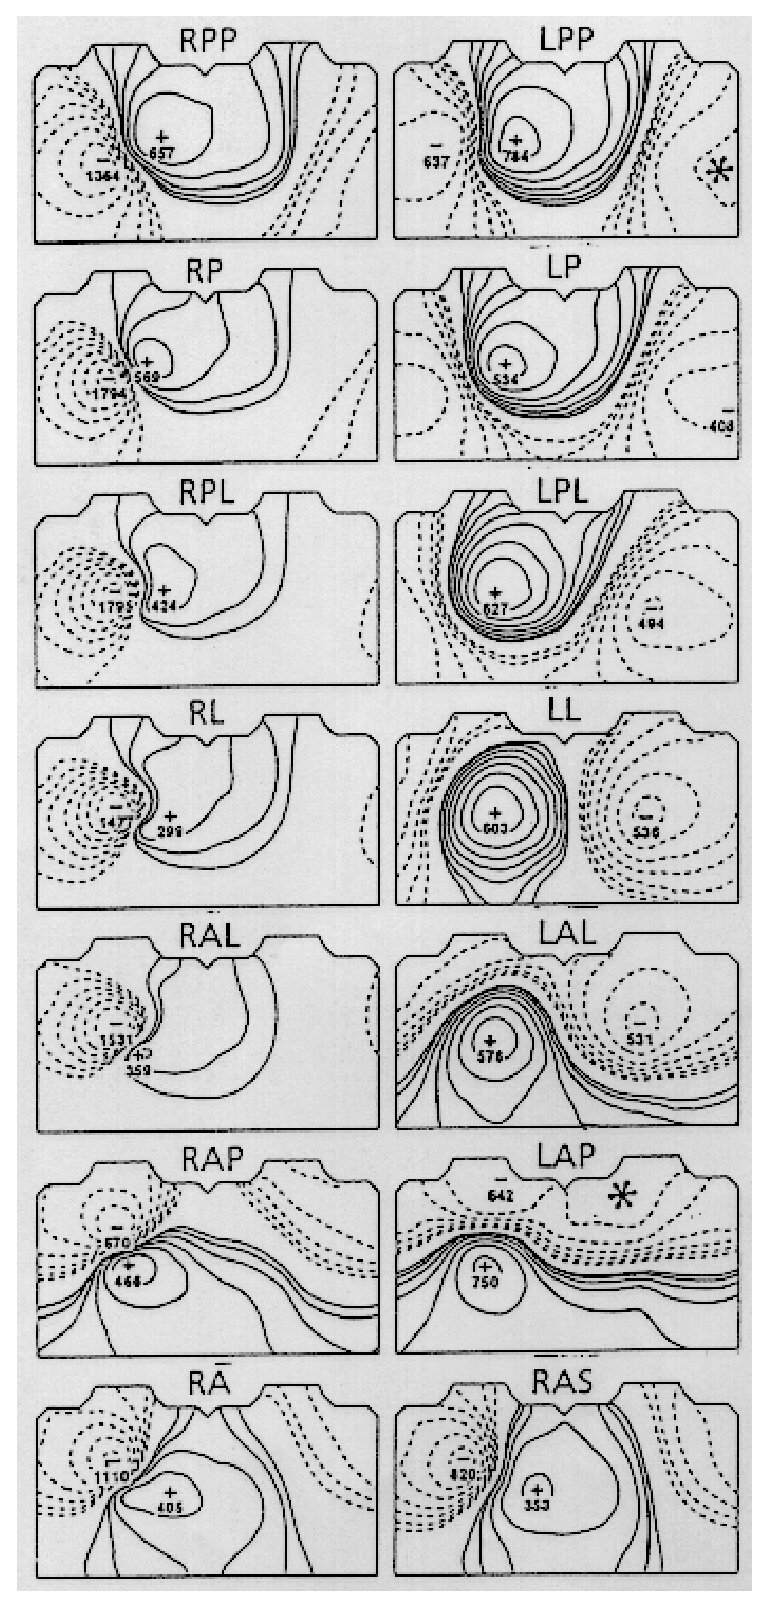
\epsfig{file=electrocardiology/epsfiles/hal-bspm-template.eps,width=8.5cm}
  \caption[Simulated WPW maps]{The simulated BSPMS at 40ms after the onset of
    stimulation which was individualy applied at the 14 preexcitation sites
    shown in  \figref{fig:hal-heart-model}.  The right and left borders of each
      map both correspond to the right mid-axillary line; the lower border
      corresponds to the waist.  Isopotential lines progress logarithmically
      and the principal extrema have their amplitudes marked in microvolts }
  \label{fig:hal-bspm-template}
\end{figure}

\begin{figure}[htbp] \centering
  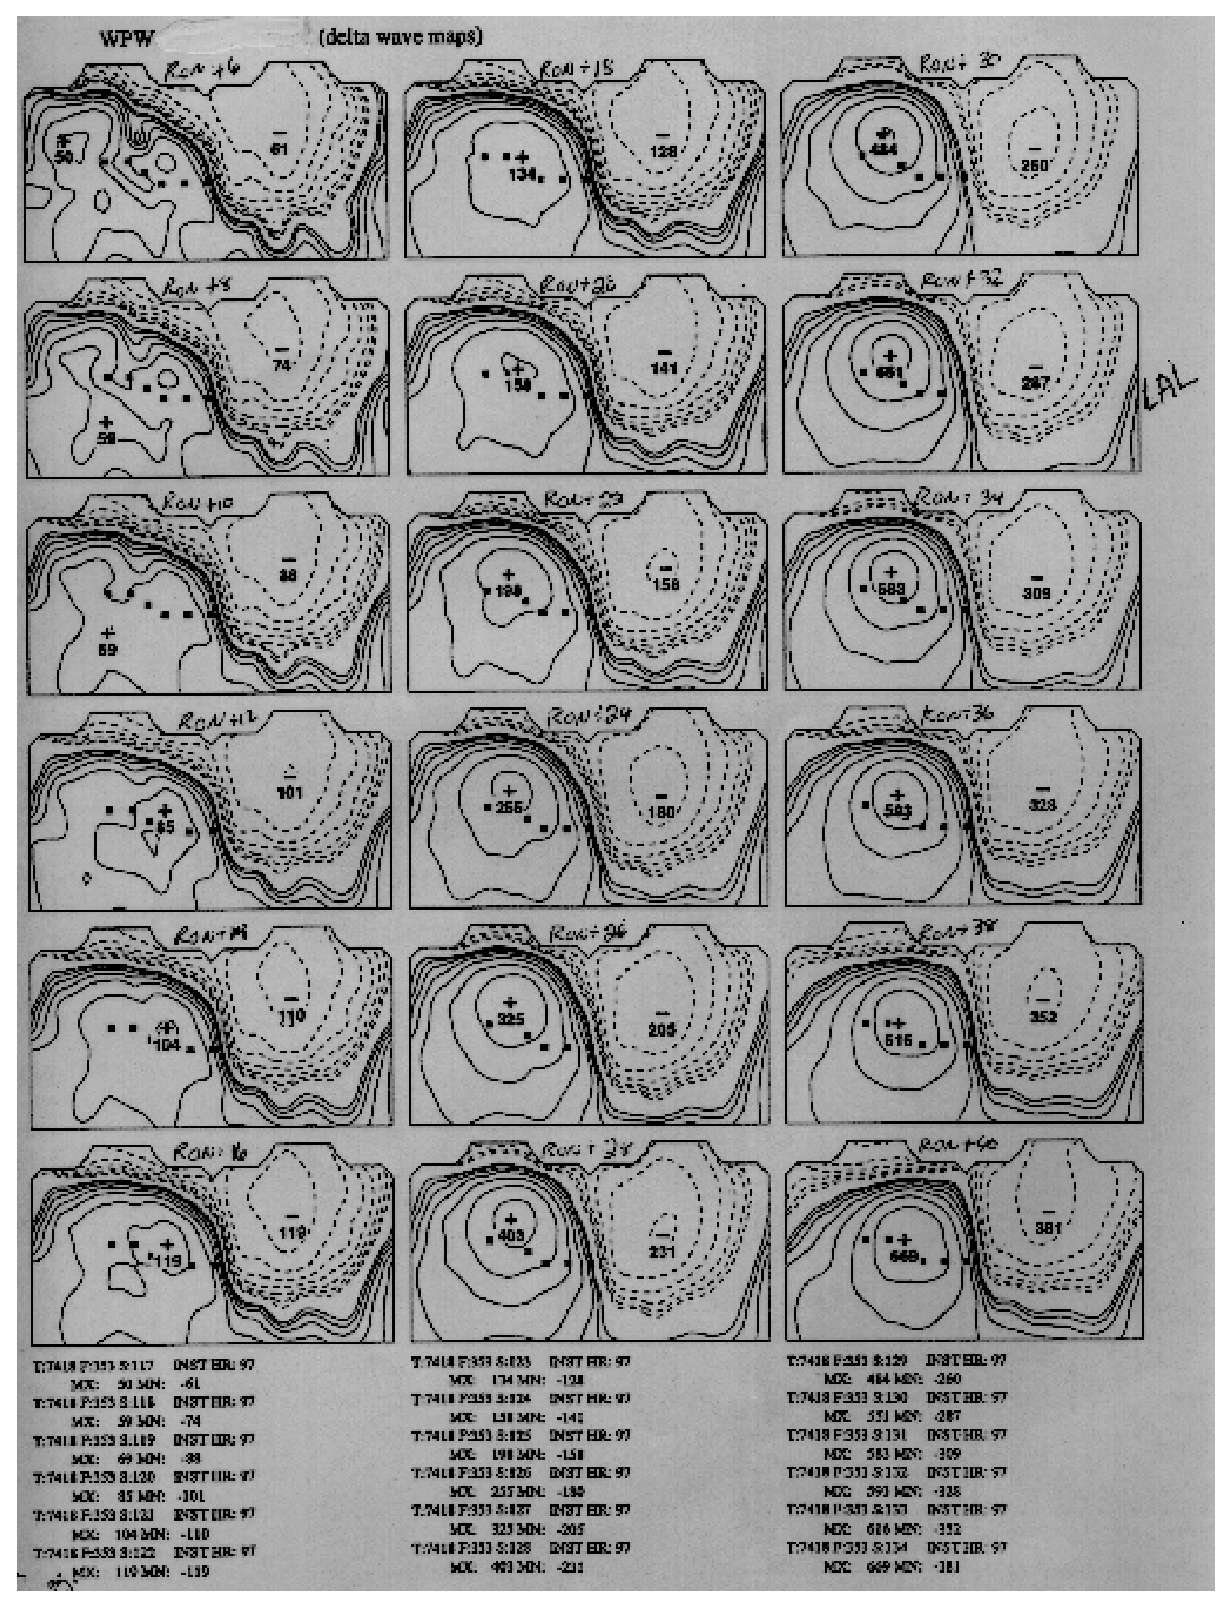
\epsfig{file=electrocardiology/epsfiles/hal-bspm-wpw1.eps,width=10cm}
  \caption[Real BSPM WPW map (a)]{A real BSPM from a WPW patient.  The accesory
    pathway is at LAL which is predicted using the template }
  \label{fig:hal-bspm-wpw1}
\end{figure}

\begin{figure}[htbp] \centering
  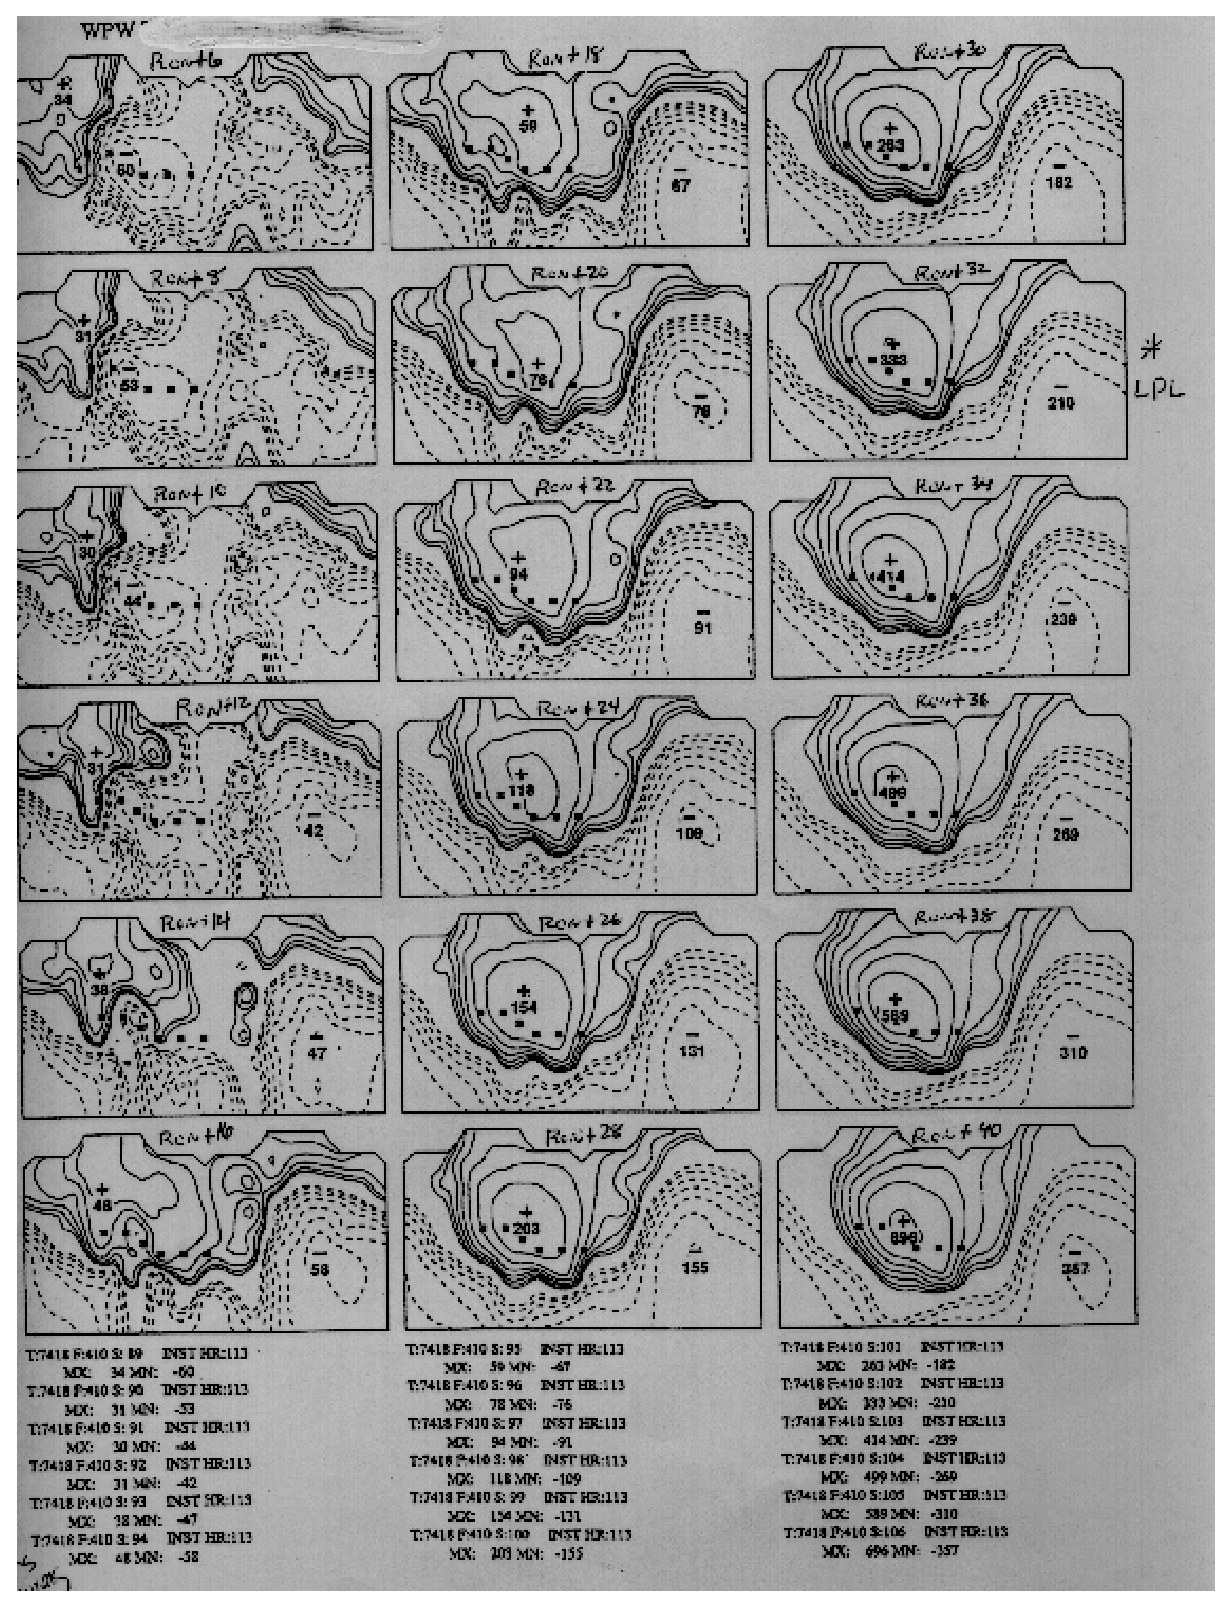
\epsfig{file=electrocardiology/epsfiles/hal-bspm-wpw2.eps,width=10cm}
  \caption[Real BSPM WPW map (b)]{Real WPW map (b) }
  \label{fig:hal-bspm-wpw2}
\end{figure}

\begin{figure}[htbp] \centering
  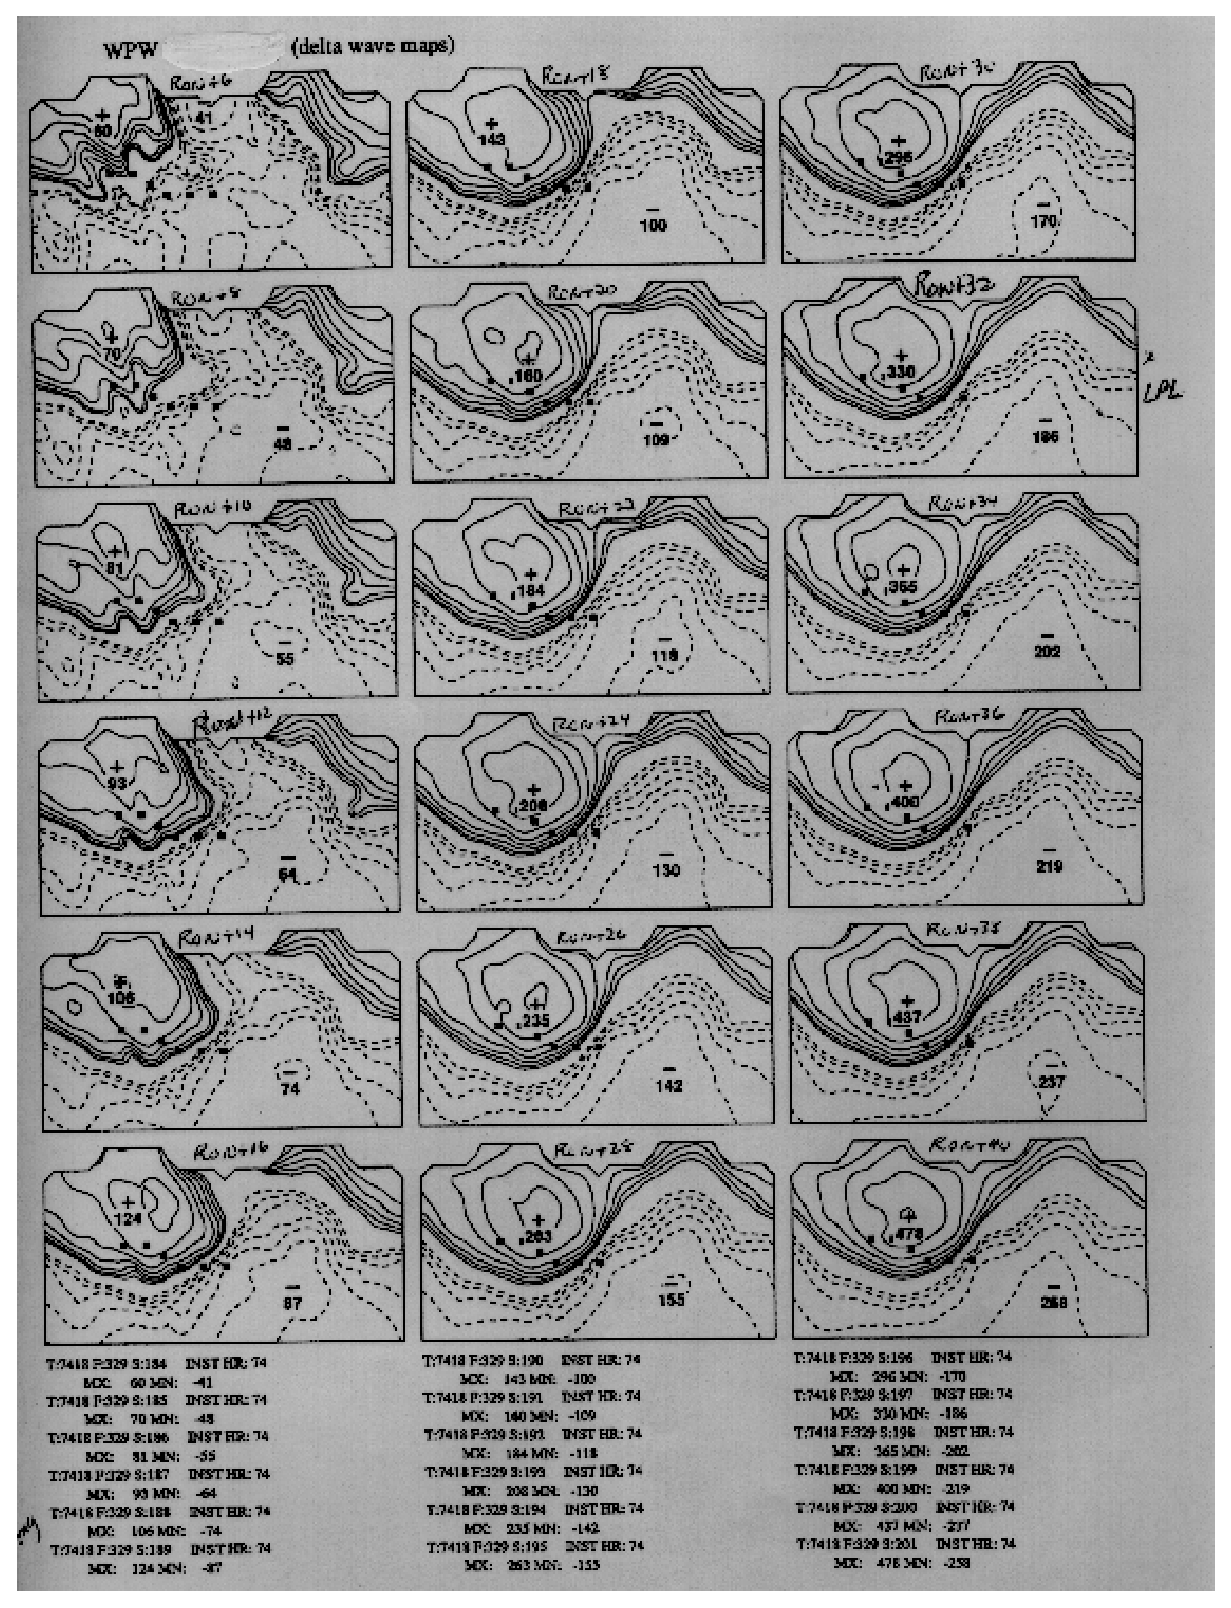
\epsfig{file=electrocardiology/epsfiles/hal-bspm-wpw3.eps,width=10cm}
  \caption[Real BSPM WPW map (c)]{Real WPW map (c) }
  \label{fig:hal-bspm-wpw3}
\end{figure}

\begin{figure}[htbp] \centering
  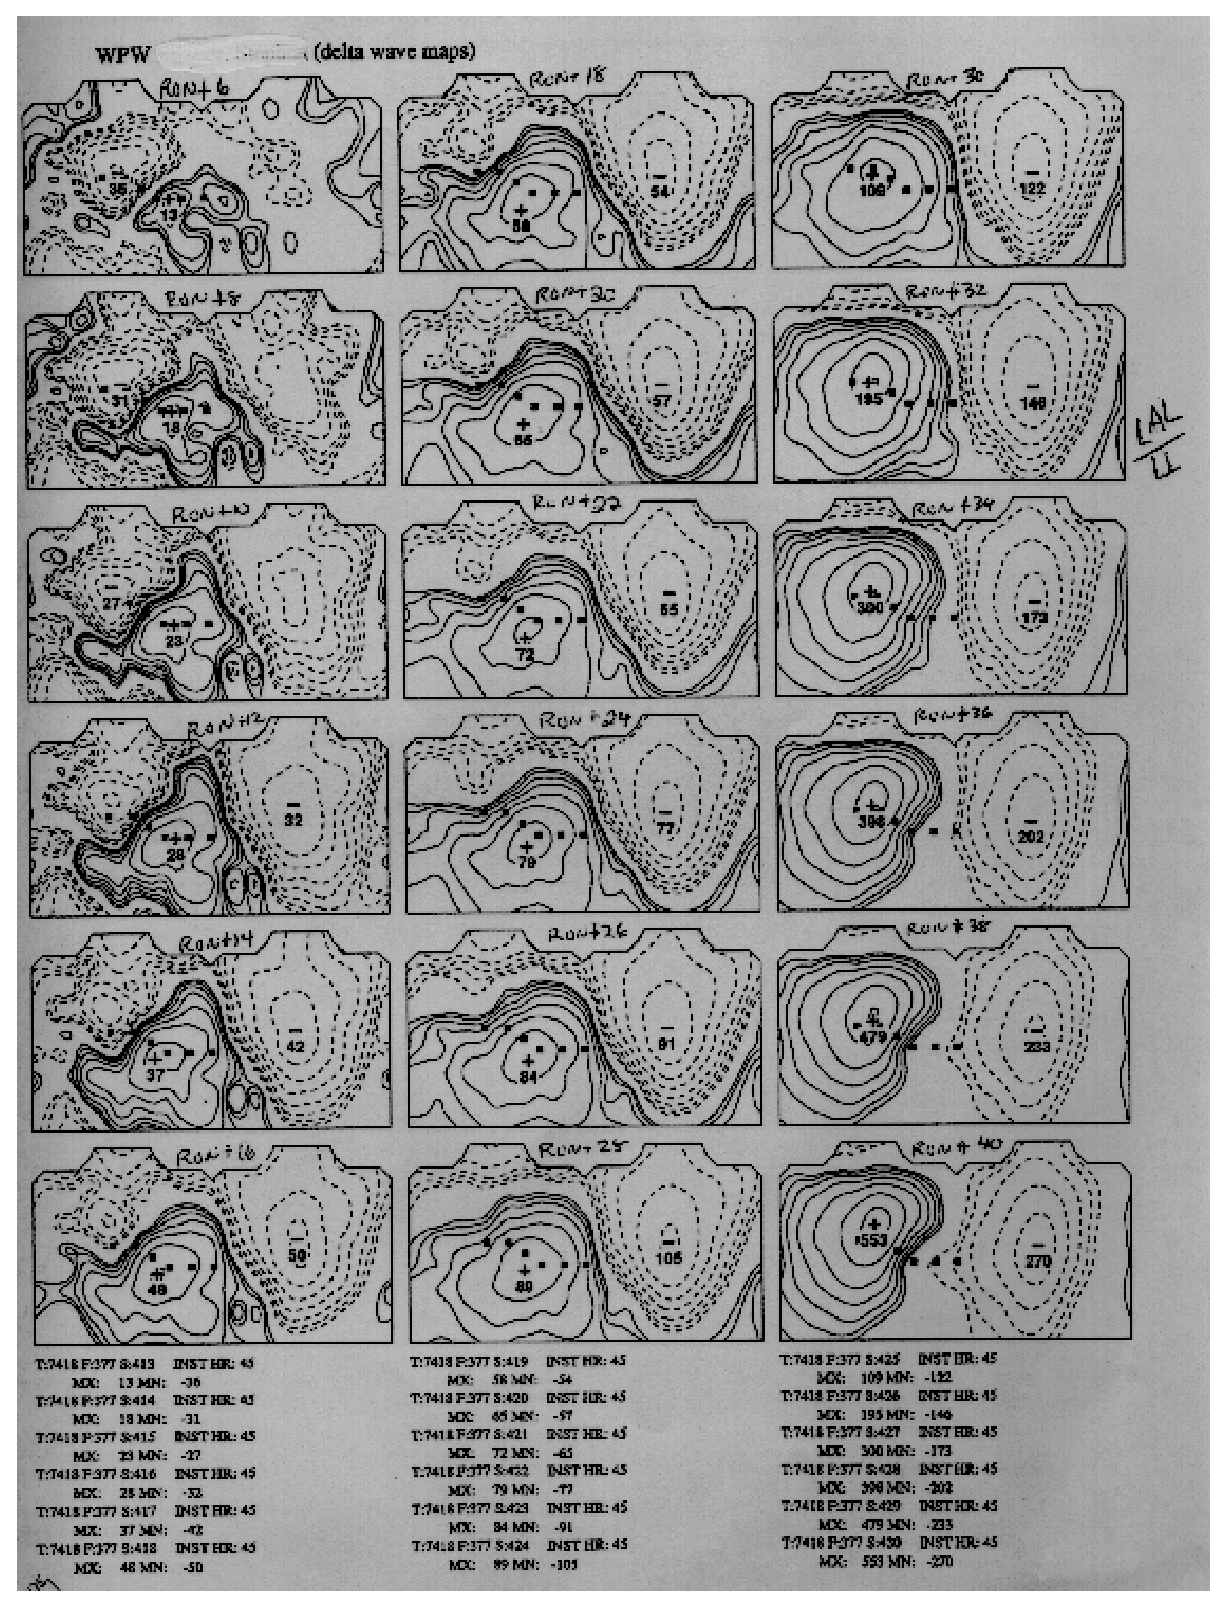
\epsfig{file=electrocardiology/epsfiles/hal-bspm-wpw4.eps,width=10cm}
  \caption[Real BSPM WPW map (d)]{Real WPW map (d). The best template match was
    LAL and LL. }
  \label{fig:hal-bspm-wpw4}
\end{figure}

\begin{figure}[htbp] \centering
  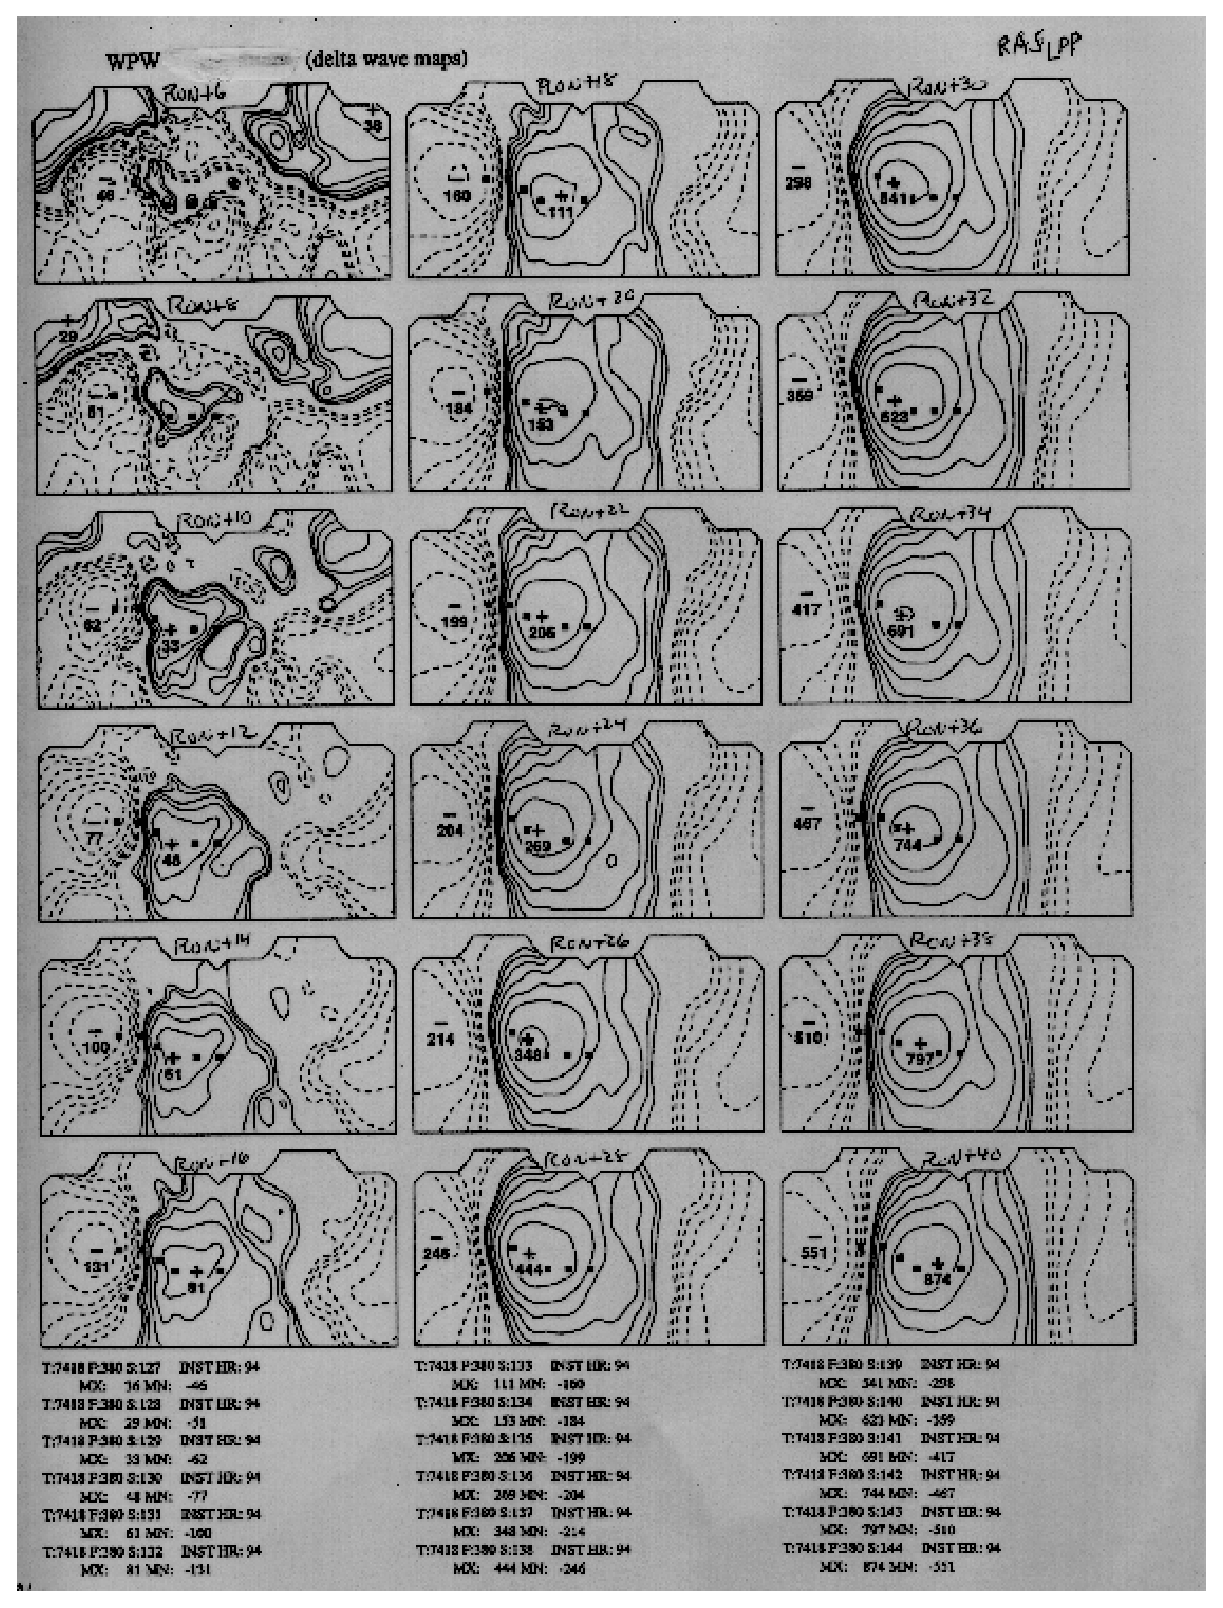
\epsfig{file=electrocardiology/epsfiles/hal-bspm-wpw5.eps,width=10cm}
  \caption[Real BSPM WPW map (e)]{Real WPW map (e).  The best template match was
   RAS and LPP}
  \label{fig:hal-bspm-wpw5}
\end{figure}

\begin{figure}[htbp] \centering
  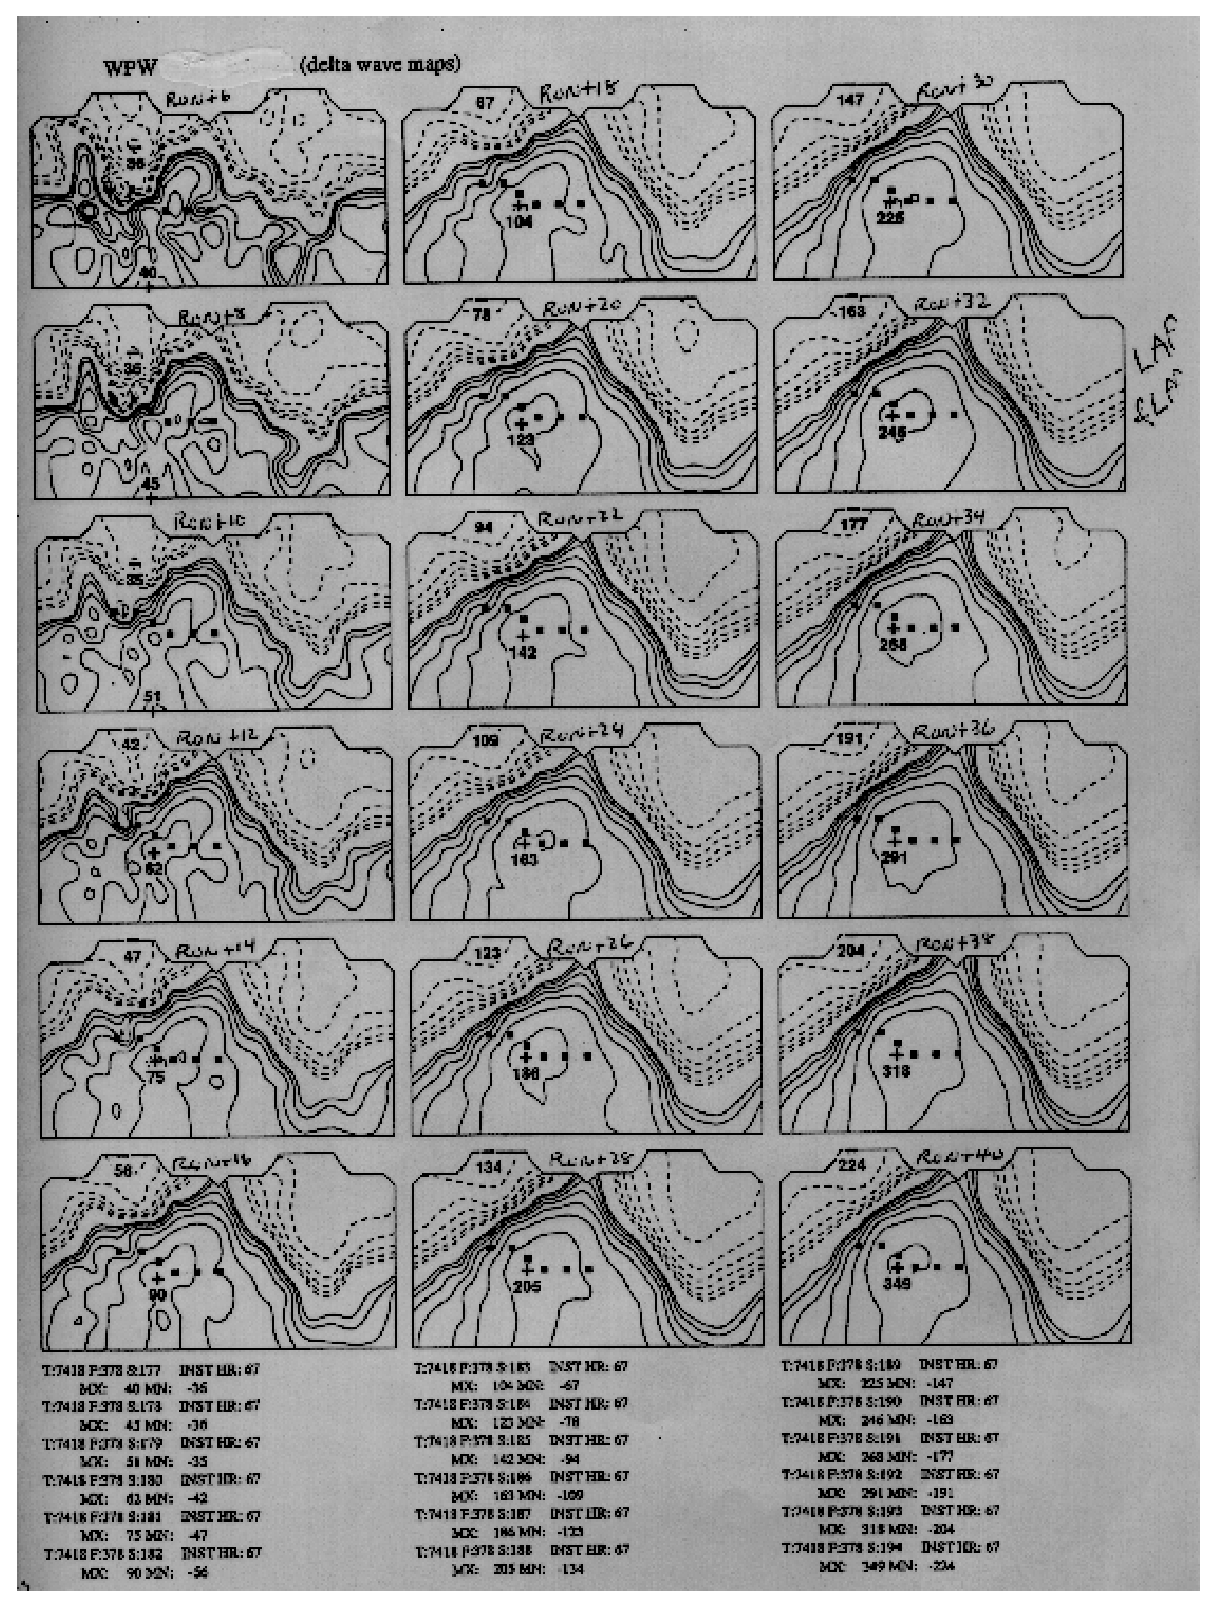
\epsfig{file=electrocardiology/epsfiles/hal-bspm-wpw6.eps,width=10cm}
  \caption[Real BSPM WPW map (f)]{Real WPW map (f).  There were 2 accesory
    pathways  at LAP and LPP }
  \label{fig:hal-bspm-wpw6}
\end{figure}

\section{The Forward and Inverse Problems of Electrocardiography}
\subsection{Introduction}
\enlargethispage{-\baselineskip}
\enlargethispage{-\baselineskip}
\enlargethispage{-\baselineskip}
The goal of non-invasive electrical imaging of the heart is to
quantitatively reconstruct information about the electrical activity
of the heart from densely sampled thoracic ECG signals. 

Quantitative interpretation of the densely sampled data in terms of the
underlying cardiac electrical activity is an inverse problem, and various
mathematical algorithms have been developed over the years in an attempt to
solve this electrical imaging problem 
e.g. \cite{barr:1978,gulrajani:1984,martin:1975,oster:1992}. Unless the problem is
posed in a particular manner this inverse problem is not uniquely determined
i.e. there exist multiple cardiac electrical generator configurations that can
give rise to the same thoracic ECG measurements. This non-uniqueness has
hampered attempts at solving the inverse problem.  Early approaches to the
inverse problem overcame the non-uniqueness by modelling the heart as a
combination of a small number of fixed or moving dipoles.  It has been
recognised that posing the problem in terms of trying to reconstruct
epicardial potentials from the body surface potential recordings is uniquely
determined. However, the reconstruction of epicardial potentials is ill-posed.
This means that in the presence of noise (which always exists) a solution to
the inverse problem produces a result which may bear no resemblance to that of
the true electrical generator.  The emergence of a general theory for such
ill-posed problems \cite{tikhonov:1977} and the introduction of the ideas
behind constraining the mathematical solutions has resulted in the large
number of variants of the inverse algorithms in existence today in the
electrical imaging area.  However, since they are based on a generic approach,
most of the modern algorithms fail to incorporate the underlying physiological
processes governing the generation of the body surface potentials (namely an
evolving wave of activation).  Most of these algorithms also do not impose the
constraints in a mathematically correct fashion
\cite{greensite:1998b,greensite:1998}.

\subsection*{A New Approach}

Another approach to the inverse problem is to pose the problem in terms of the
underlying activation sequence \cite{huiskamp:1988}. This has significant advantages
over the epicardial potential problem formulation, not least in that it deals
directly with the underlying physiological process responsible for generating the
body surface potentials. However, it introduces additionally difficulties in the
modelling process (for instance the need to accurately model the entire heart instead
of just modelling the epicardial surface).  Because of this, and partly because of
the fact that an appropriate algorithm for such a problem formulation had
previously not been devised, this approach has not found much favour.
However, a powerful new algorithm, based on this activation imaging approach
has recently emerged \cite{greensite:1998b,huiskamp:1997}.

Both the epicardial and activation source formulations mentioned above have
been recognised for twenty to thirty years but as of yet no clinically
acceptable imaging techniques have resulted. The two major reasons for this
are
\begin{enumerate}
\item Previously available mathematical methodologies for computation of the
  sources were not powerful enough.
\item Adequate procedures for verification of the accuracy of the images were
  not employed.
\end{enumerate}
For each of the two source formulations there are now powerful imaging
algorithms that have not previously been available, 
e.g. \cite{greensite:1998b,greensite:1998,huiskamp:1997}. There are also
sufficient modelling techniques now available that when combined with these new
algorithms should make it possible to produce myocardial electrical source images of
sufficient stability and accuracy to be a useful adjunct in the clinical
assessment of the heart. However, these new algorthims need to be quantitatively
validated before teh clinical worth can be properly assessed.

In order to quantitatively validate the performance of the inverse procedures, one
needs to compare any mathematical results against experimentally-obtained 
\emph{invivo} data, in particular simultaneously recorded densely sampled body
surface and cardiac potentials.  This has rarely been attempted -- rather the
worth of various inverse procedures has often been judged by examining the
performance on simulated data or in \emph{in vitro} torso tank experiments.  As
far as is known, only two sets of \emph{invivo} data have ever been collected, one
in a chimpanzee \cite{spach:1979} (in which no inverse solution was attempted)
and one in a dog \cite{barr:1978}.  Neither set is currently available.  Data
from \emph{in vitro} experiments from perfused canine hearts in a homogeneous
cylindrical tank have been collected by Taccardi \emph{et. al.} and are in use by that
group and others \cite{oster:1992,oster:1997,oster:1998}.

We are currently performing experiments on pigs to provide the necessary \emph{invivo}
data to validate the new inverse procedures.  We present here the details of
the underlying theory behind the electrical imaging process and the porcine
model development.  We also illustrate how the procedure is to be applied in
practice by producing an inversely-reconstructed cardiac surface activation
map from simulated data.  
%A companion paper will focus on the experimental
%procedure and the quantitative validation of this inverse reconstruction from
%experimental \emph{invivo} data.


%%%%%%%%%%%%%%%%%%%%%%%%%%%%%%%%%%%%%%%%%%%%%%%%%%%%%%%%%%%%%%%%%%%%%%%%%%%%%%%
%% Theory
%%%%%%%%%%%%%%%%%%%%%%%%%%%%%%%%%%%%%%%%%%%%%%%%%%%%%%%%%%%%%%%%%%%%%%%%%%%%%%%

\section{Theory}
\enlargethispage{\baselineskip}
The basic activation inverse algorithm is presented in Huiskamp and 
Greensite \cite{huiskamp:1997}.
The procedure revolves around the identification of the critical
points and times of the surface activation function (i.e. epi- and
endocardial breakthrough/termination points and times) via the use of
a modified MUSIC algorithm.  To use this method on a given
individual/animal requires the construction of an appropriate transfer
function or mapping from the activation sequence to body surface
potentials.

The proof of the activation imaging algorithm \cite{greensite:1998b} uses
source field relationships given in \cite{yamashita:1985}.  These
relationships employ a Green's function that takes into account the anisotropy
of the myocardium.  While the new imaging algorithm proved from these
relationships is completely general, the initial use of it has been restricted
to using the so-called double layer transfer matrices, which assume a
homogeneous and
isotropic heart muscle.  The traditional construction of such a double-layer
transfer matrix begins with the assumption of myocardial homogeneity and
isotropy and the use of equations defining the potential due to a dipole in
freespace \cite{cuppen:1984}. We prefer to investigate the transfer matrix
construction from a boundary value problem point of view (e.g. from solving
the bidomain equations) which avoids explicit reference to dipoles, and makes
more explicit the anisotropic/isotropic distinction.  This approach also
generalises some of the identities presented in \cite{yamashita:1985}.

\subsection{Transfer Matrices From A Boundary Value Problem Point of View}
Let $D_{H}$ be the domain of the heart, $S_{H}=$ $\partial D_{H}$ (closed),
$\phi _{i}$ the intracellular potential,
$\phi _{e}$ the extracellular potential,
$\phi _{m}$ the transmembrane potential ($=$ $\phi _{i}-\phi _{e}$ ),
$\phi $ the torso potential outside $D_{H}$ and
$\overline{G_{i}}$ and $\overline{G_{e}}$ the intracellular and
extracellular conductivity tensors.

From bidomain theory we have inside $D_{H}$

\begin{equation}
\nabla \cdot ([\overline{G_{i}}+\overline{G_{e}}]\nabla \phi _{e})=-\nabla
\cdot (\overline{G_{i}}\nabla \phi _{m})  \label{current_cons}
\end{equation}

This is a Poisson equation for $\phi _{e}$ in which the source term is $%
-\nabla \cdot (\overline{G_{i}}\nabla \phi _{m}).$

One can solve this partial differential equation using a weighted residuals approach. 
Let $w$ be a (as-yet-unspecified) weighting function. Then, from weighted residuals

\begin{equation}
0=\int_{D_{H}}\nabla \cdot ([\overline{G_{i}}+\overline{G_{e}}]\nabla \phi
_{e})wd\Omega +\int_{D_{H}}\nabla \cdot (\overline{G_{i}}\nabla \phi
_{m})wd\Omega  \label{weighted_resid}
\end{equation}

Using Green's theorem we get
%%
\begin{equation}
0=\int_{S_{H}}w[\overline{G_{i}}+\overline{G_{e}}]\nabla \phi _{e}\cdot
ndS-\int_{D_{H}}[\overline{G_{i}}+\overline{G_{e}}]\nabla \phi _{e}\cdot
\nabla wd\Omega +\int_{D_{H}}\{\nabla \cdot (\overline{G_{i}}\nabla \phi
_{m})\}wd\Omega  \label{Start_fem_eqtn}
\end{equation}
where $n$ is the unit outward normal.

Applying Green's theorem again, one gets 
\begin{multline}
        0 =\int_{S_{H}}w[\overline{G_{i}}+\overline{G_{e}}]\nabla \phi _{e}\cdot
        ndS-\int_{S_{H}}\phi _{e}[\overline{G_{i}}+\overline{G_{e}}]\nabla w\cdot
        ndS  \\
        + \int_{D_{H}}\nabla \cdot ([\overline{G_{i}}+\overline{G_{e}}]\nabla w)
        \phi_{e}d\Omega +\int_{D_{H}}\nabla \cdot (\overline{G_{i}}\nabla 
        \phi_{m})wd\Omega   
        \label{Start_bem_eqtn}
\end{multline}

This is the standard boundary integral equation for Poisson's equation with
a general source term. For the special case of the source being given by $-%
\nabla \cdot (\overline{G_{i}}\nabla \phi _{m})$ we can apply a similar
procedure to that above on this term i.e. 
\begin{eqnarray}
\int_{D_{H}}\nabla \cdot (\overline{G_{i}}\nabla \phi _{m})wd\Omega 
        &=&\int_{S_{H}}w\overline{G_{i}}\nabla \phi _{m}\cdot ndS-\int_{D_{H}}
        \overline{G_{i}}\nabla \phi _{m}\cdot \nabla wd\Omega   \nonumber \\
        &=&\int_{S_{H}}w\overline{G_{i}}\nabla \phi _{m}\cdot ndS 
                -\int_{S_{H}} \phi_{m}\overline{G_{i}}\nabla w\cdot ndS  \nonumber \\
                && \quad + \int_{D_{H}}\nabla \cdot (\overline{G_{i}}\nabla w)\phi _{m}d\Omega 
        \label{source_term}
\end{eqnarray}

Inserting \eqnref{source_term} into \eqnref{Start_bem_eqtn} we get

\begin{eqnarray}
        0 &=&\int_{S_{H}}w[\overline{G_{i}}+\overline{G_{e}}]\nabla \phi _{e}\cdot ndS
                -\int_{S_{H}}\phi _{e}[\overline{G_{i}}+\overline{G_{e}}]\nabla w\cdot ndS 
                          \nonumber \\
                && \quad
                        + \int_{D_{H}}\nabla \cdot ([\overline{G_{i}}+\overline{G_{e}}]\nabla w)
                        \phi_{e}d\Omega +\int_{S_{H}}w\overline{G_{i}}\nabla \phi _{m}\cdot ndS 
                        \nonumber \\
                && \quad 
                        - \int_{S_{H}}\phi _{m}\overline{G_{i}}\nabla w\cdot ndS+\int_{D_{H}}\nabla
                        \cdot (\overline{G_{i}}\nabla w)\phi _{m}d\Omega   
        \label{BIE eqtn}
\end{eqnarray}

which is a generalisation of Equation 31 of \cite{yamashita:1985}.

This \eqnref{BIE eqtn} is general - no assumptions (apart from
differentiability and integrability) have been made on $w,\overline{G_{i}}\ $%
or $\overline{G_{e}}$. In \cite{yamashita:1985}, they
assumed that $w$ was a Green's function satisfying

\begin{equation}
\nabla \cdot ([\overline{G_{i}}+\overline{G_{e}}]\nabla w)+\delta (P)=0
\label{Greens_fn}
\end{equation}

and 
\begin{equation}
\lbrack \overline{G_{i}}+\overline{G_{e}}]\nabla w\cdot n=0\text{ on }S_{B}
\text{ }  \label{no_flux}
\end{equation}

where $\delta (P)$ is the Dirac delta distribution centred at a point $P$ and
$S_{B}$ is the surface of the torso.  This resulted in the removal of the
first volume integral in \eqnref{BIE eqtn}.

In practice, such a Green's function for the heart cannot be found
analytically, since both $\overline{G_{i}}$ and $\overline{G_{e}}$ 
are in general anisotropic and inhomogeneous.
If one assumes that they are homogeneous then both conductivity tensors can be
represented by a constant $3\times 3$ matrix, which is diagonal in the coordinate
system defined by the myocardial fibres and sheets. The fibre/sheet orientation in
the heart is very complex, which means that it is not possible in practice to solve
\eqnref{Greens_fn} analytically even under the assumption of homogeneity, or
even equal anisotropy ratios (i.e. $G_{i}=kG_{e}$ where $k$ is a constant).
This is true irrespective of whether we strive for a proper Green's function
(i.e. impose \eqnref{no_flux}) or merely look for a freespace Green's
function (also known as a fundamental solution) which is a solution of
\eqnref{Greens_fn} with zero boundary conditions at infinity (i.e. the no-flux
condition on $S_{B}$ is ignored).

If one assumes further that the domain is isotropic in both the extra and intracellular
domains, then one can apply a standard boundary element procedure to 
\eqnref{BIE eqtn}. For this we take $w$ to be the freespace Green's function 
i.e. a solution of
\begin{equation}
\nabla \cdot ([(1+k)G_{e}]\nabla w)+\delta (P)=0
\label{Fundamental_soln_eqtn}
\end{equation}

subject to zero boundary conditions at infinity. In three-dimensions, the
solution of this equation is
\begin{equation}
w=\frac{1}{4\pi (1+k)G_{e}R}  \label{Fundamental_soln}
\end{equation}

where $R$ is the distance measured from $P$. 

With $w$ defined as above, we get, for $P$ inside $D_{H}$

\begin{eqnarray}
\int_{D_{H}}\nabla \cdot ([\overline{G_{i}}+\overline{G_{e}}]\nabla w)\phi
_{e}d\Omega  &=&\int_{D_{H}}\nabla \cdot ([(1+k)G_{e}]\nabla w)\phi
_{e}d\Omega   \nonumber \\
&=&-\phi _{e}(P)  \label{Volume_int_phie}
\end{eqnarray}

and 
\begin{eqnarray}
\int_{D_{H}}\nabla \cdot (\overline{G_{i}}\nabla w)\phi _{m}d\Omega 
&=&\int_{D_{H}}\nabla \cdot (kG_{e}\nabla w)\phi _{m}d\Omega   \nonumber \\
&=&-\frac{k}{k+1}\phi _{m}(P)  \label{Volume_int_phim}
\end{eqnarray}

So \eqnref{BIE eqtn} becomes 
\begin{eqnarray}
0 &=&\int_{S_{H}}w(1+k)G_{e}\nabla \phi _{e}\cdot ndS-\int_{S_{H}}
        \phi_{e}(1+k)G_{e}\nabla w\cdot ndS-\phi _{e}(P)  \nonumber \\
        &&\quad +\int_{S_{H}}wkG_{e}\nabla \phi _{m}\cdot ndS-\int_{S_{H}}
        \phi_{m}kG_{e}\nabla w\cdot ndS-\frac{k}{k+1}\phi _{m}(P)
        \label{BIE_eqtn_p_inside}
\end{eqnarray}

The equation of more interest is the case for when $P\in S_{H}$ (i.e. $P$ is
on the boundary of the domain). To derive this equation, consider $P$ at a
smooth point on the
boundary of $D_{H}$ and construct a hemispherical region of radius $%
\varepsilon $ centred at $P$ . Let $D_{H}^{^{\prime }}$ be the extended
region (i.e. $D_{H}$ with the hemispherical region). Then $P$ is interior to 
$D_{H}^{^{\prime }}$ so \eqnref{BIE_eqtn_p_inside} is valid with $S_{H}$
replaced by $\partial D_{H}^{^{\prime }}$. One now considers this equation
in the limit as $\limita{\varepsilon}{0}{}$. If $\Gamma _{\varepsilon }$
is the boundary of the hemispherical region, and $\Gamma _{-\varepsilon }$
the boundary of that part of $D_{H}$ that is outside the hemisphere (so $%
\partial D_{H}^{^{\prime }}=$ $\Gamma _{\varepsilon }\cup \Gamma
_{-\varepsilon }$) then we find that

\begin{eqnarray}
        \limita{\varepsilon}{0}{\int_{\Gamma _{\varepsilon }}
        \phi_{e}(1+k)G_{e}\nabla w\cdot ndS}
        &=&
        \limita{\varepsilon}{0}
                {-\frac{1}{4\pi R^{2}}2\pi R^{2}\phi _{e}(\gamma )}\nonumber \\
        &=& -\frac{\phi_{e}(P)}{2}
        \label{limit1}
\end{eqnarray}

where $\gamma $ is some point on the hemisphere of radius $\varepsilon $
(the mean value theorem has been applied).

Similarly 
\begin{eqnarray}
\limita{\varepsilon}{0}
        {\int_{\Gamma _{\varepsilon }}\phi_{m}kG_{e}\nabla w\cdot ndS}
        &=&
        \limita{\varepsilon}{0}
                {-\frac{k}{k+1}\frac{1}{4\pi R^{2}}2\pi R^{2}\phi _{m}(\gamma )}  \nonumber \\
                &=&
        -\frac{k}{k+1}\frac{\phi _{m}(P)}{2}
        \label{limit2}
\end{eqnarray}

It can also be shown that 
\begin{equation}
        \limita{\varepsilon}{0}
                {\int_{\Gamma _{\varepsilon}}w(1+k)G_{e}\nabla \phi _{e}\cdot ndS}=0
        \label{limit3}
\end{equation}

and 
\begin{equation}
        \limita{\varepsilon}{0}
        {\int_{\Gamma _{\varepsilon}}wkG_{e}\nabla \phi _{m}\cdot ndS} =0
        \label{limit4}
\end{equation}

As $\limita{\varepsilon}{0}{}$ and $\limita{\Gamma _{-\varepsilon}}{S_{H}}{}$ and
while the integrands are singular, the integrals exist in the 
standard sense, so one can write 
\begin{equation}
        \limita{\varepsilon}{0}
        {\int_{\Gamma_{-\varepsilon}}(\text{each integrand})dS}
        =\int_{S_{H}}(\text{same integrand})dS  
        \label{limit5}
\end{equation}

Using \eqnref{limit1} to \eqnref{limit5} together with \eqnref{BIE_eqtn_p_inside}
we obtain the general boundary integral equation 
\begin{multline}
        c(P)\phi _{e}(P)+\frac{k}{k+1}c(P)\phi _{m}(P)+   
        \int_{S_{H}}\phi _{e}(1+k)G_{e}\nabla w\cdot ndS+   
        \int_{S_{H}}\phi _{m}kG_{e}\nabla w\cdot ndS                    \\
        =\int_{S_{H}}w(1+k)G_{e}\nabla \phi _{e}\cdot ndS +
        \int_{S_{H}}wkG_{e}\nabla \phi _{m}\cdot ndS  
        \label{BIE eqtn_final}
\end{multline}

where 
\begin{equation}
c(P)=\left\{ 
\begin{array}{l}
1\text{ if }P\in D_{H}^{0} \\ 
\frac{1}{2}\text{ if }P\in S_{H}\text{ and }S_{H}\text{ smooth at }P \\ 
\frac{\text{internal solid angle}}{4\pi }\text{ if }P\in S_{H}\text{ and }%
S_{H}\text{ not smooth at }P \\ 
0\text{ if }P\ \text{outside }D_{H}
\end{array}
\right.  \label{cp}
\end{equation}

\eqnref{BIE eqtn_final} relates $\phi _{e}$ and $\phi _{m}$ at a
point to the values of $\phi _{e},\phi _{m},\nabla \phi _{e}\cdot n$ and $%
\nabla \phi _{m}\cdot n$ everywhere on $S_{H}$.  
On $S_{H}$, $\nabla \phi_{m}\cdot n$ is $0$ since transmembrane potentials are
confined to the heart, which removes the last integral in \eqnref{BIE eqtn_final}.

Outside the
heart, the governing equation is
\begin{equation}
        \nabla \cdot (\sigma \nabla \phi )=0  
        \label{Gen_Laplace}
\end{equation}
 and this can be solved using a coupled Finite Element/Boundary Element
 procedure \cite{pullan:1996b}.  Continuity of (extra-cellular) potential and
 current across the myocardial boundaries provides the links between
 \eqnref{Gen_Laplace} and \eqnref{BIE eqtn_final}.
In the usual way, one can discretise the boundaries of all regions involved,
and assemble the following matrices 
\begin{equation}
\left( 
\begin{array}{c}
        \text{all coefficients } \\ 
        \text{of potentials from} \\
        \text{\eqnref{BIE eqtn_final} }\\
        \text{and \eqnref{Gen_Laplace} }
\end{array}
\right) \left( 
\begin{array}{c}
        \vect{\phi _{m}}                 \\ 
        \vect{\phi _{e}^{H}} \\ 
        \vect{\phi _{e}^{1}} \\ 
        . \\ 
        . \\ 
        \vect{\phi_{e}^{\uppercase{N}}}
\end{array}
\right) =\left( 
\begin{array}{c}
        \text{all coefficients } \\ 
        \text{of currents from}  \\
        \text{\eqnref{BIE eqtn_final} } \\
        \text{and \eqnref{Gen_Laplace} }        
\end{array}
\right) \left( 
\begin{array}{c}
        (1+k)G_{e}\frac{\partial  \vect{\phi_{e}^{\uppercase{H}}}}{\partial n}  \\ 
        \sigma ^{1}\frac{\partial \vect{\phi_{e}^{1}}}{\partial n} \\ 
        . \\ 
        . \\ 
        \sigma ^{N}\frac{\partial \vect{\phi_{e}^{i}}}{\partial n}
\end{array}
\right)  
\label{global_system}
\end{equation}

\begin{equation*}
\begin{split}
\text{where} & \\
\quad\quad &N   \quad \text{is a number of regions outside the heart} \\
                &\vect{\expot^i}
                                \quad \text{is a vector of nodal values of \expot in region $i$}\\
                &\vect{\tranpot}
                                \quad \text{is a vector of nodal values of \tranpot in the heart}\\
                &\vect{\expot^{\uppercase{H}}}
                                \quad \text{is a vector of nodal values in the heart}   \\
                &\sigma^i       \quad \text{is the conductivity in region $i$}          
\end{split}
\end{equation*}


The coefficient matrices include all the continuity constraints. Also, since
\delby{\vect{\tranpot}}{n} is $0$ on $S_H$, this term is not present in
\eqnref{global_system}. It is worth noting
that the coefficients of \vect{\tranpot} in \eqnref{BIE eqtn_final} are just
$\frac{k}{k+1}$ times the coefficients of \vect{\phi_{e}} in that equation.  Use
of this fact allows one to speed up the assembly of \eqnref{global_system}

\Eqnref{global_system} above can be considered to be an implicit
relationship between \vect{\tranpot} and the torso potentials \vect{\bodypot}.
To construct an explicit transfer matrix $A$ from \vect{\tranpot} to 
\vect{\bodypot} one simply needs to set \vect{\tranpot} to be the vector 
$\vect{e_{k}}$ (i.e. a unit vector that is zero everywhere except at the $k^{th}$
position) and solve \eqnref{global_system}. The resulting solution for
\vect{\bodypot} will correspond to the $k^{th}$ column of $A$ 
(since $\vect{\bodypot} = A \vect{\tranpot}$).
Alternatively one can construct a transfer matrix from \vect{\tranpot}
to $\vect{\expot^{\uppercase{H}}}$ by suitable rearrangement of
\eqnref{global_system}. 

No mention has yet been made of the singular nature or otherwise of
\eqnref{global_system}. The physical problem being solved suggests that
\eqnref{global_system} will be singular if \vect{\tranpot} is the only variable to be 
specified, since no potential reference has been given. The system can either be
solved in a least-squares sense, or a technique such as deflation used. 

The construction of the transfer matrix described above has assumed homogeneity and
isotropy in the heart muscle from \eqnref{BIE eqtn} onwards. It is worth pointing
out that the assumptions of homogeneity and isotropy is not required to use
the activation imaging algorithm of \cite{huiskamp:1997}.  It is also possible to
construct a transfer matrix relating activation times to torso potentials without
these assumptions as well. However, the transfer matrix construction under
anisotropic conditions becomes significantly more difficult.  The bidomain equations
(or a weak form of them, such as that given in \eqnref{BIE eqtn} have to be solved
throughout the heart (using some volume-discretisation procedure representing the
full myocardial-fibre orientation) and coupled to solutions of \eqnref{Gen_Laplace}
outside the heart. Work on this is progressing \cite{pullan:1998b} but at this
stage homogeneity and isotropy is assumed. 


\subsection{Myocardial Inverse Procedure}

The activation inverse procedure that is used here 
is described in detail in \cite{huiskamp:1988}.  We include here a summary
of that method for completeness. 

The basic idea behind the new approach stems from the observation that when
an  evolving cardiac activation wavefront intersects the epicardial surface
a \emph{hole} develops in the wavefront. This is a signifcant change to the
topology of the wavefront and thischange is reflected in the surface
potential recordings. If \activfn{x} is defined to be the
activation time on $S_H$, then these breakthough points are critical
points of of \activfn{x}; that is $\grad \activfn{\critpoint}=0$ when
\vect{\critpoint} is a breakthough point, i.e. \activfn{\critpoint} is the
breakthough or critical point.

This critical point observation leads, after much mathematical work
\cite{greensite:1995}, to the two following important results,

\begin{enumerate}
        \item \vect{\critpoint} is a critical point of \activfn{x} with critical time
                \activfn{\critpoint} $\Longleftrightarrow$ \fnof{A}{\critpoint,y} is in
                the space spanned by the spatial eigenfunctions of \bodypot, where \transfer is
                the transfer matrix from \tranpot to \bodypot.
        \item With all critical points of \activfn{x} determined, the
                computation of \activfn{x} (on both the epicardial and endocardial
                surfaces) is a well-posed problem.
\end{enumerate}

The key assumption required to prove the first point above is that
\tranpot is modelled as a uniform step jump across the wavefront.
i.e.
\begin{equation}
        \tranpot = a + b \fnof{H}{t-\activfn{x}}
\end{equation}
This assumption is not a
practical restriction for normal hearts but it does provide a measure of
the expected spatial resultion of this approach.

To compute the critical points and times we require both the signal
matrix, \PHI, recorded from surface electrodes where $t \in [0,T]$
and $y$ is a point on the torso surface and the transfer matrix from \tranpot
to \bodypot, \transfer. To determine the spactial eigen
functions of \PHI we used the singular value decomposition.
\begin{equation}
  \PHI = U \thinspace \Sigma \thinspace  V^T \quad \text{with an effective rank $R$}
\end{equation}
Eigen functions corresponding to \emph{small} singular values we discarded.
These discarded eigenfunctions are assumed to represent only noise space.

A distance from signal space can be contructed by,
\begin{equation}
  \fnof{{M}_0^T}{x} = \pbrac{1-
        \dsuml{r=1}{R} \sqbrac{\fnof{a}{x,y} \cdot \fnof{U_r}{y}}^2 }^{-1}
\end{equation}

where $\fnof{a}{x,y} = \dfrac{\transfer}{\lnorm{y}{\transfer}}$.

This distance meaure greately exaggerates points \vect{x} which are close
to signal space. This (near) singularities in \fnof{M_0^T}{x} has no
singularities due to noise and error associated with $\matr{\Phi}$ and $\matr{A}$.


To find the activation times corresponding to these critical points, we
contruct the functions,
\begin{align}
  \fnof{M^+}{x,t} &= \fnof{M_0^t}{x} \\
  \fnof{M^-}{x,t} &= \fnof{M_suaht^T}{x}
\end{align}
where $0<t<T$. These two functions look at the distance from signal space
where signal spaces are restricted to $[0,t]$ and $[t,T]$ respectively.

The zero-crossing function defined by,
\begin{equation}
        \ZCROSS=\fnof{M^+}{\vect{x},t}-\fnof{M^-}{\vect{x},t}
\end{equation}
theoretically crosses zero at the critcal time and has a large gradient
about zero.

With critical points and time identified, the process of determinging
\activfn{x} everywhere is theoretically a well-posed problem. This process
was formulated as a minimisation problem, where the objective was
to minimise the difference between calculated torso potentials \estpot,
and the measured potentials, \recpot. \estpot was calculated using
\transfer and an initial guess of \activfn{x}.

In practice, \ZCROSS provides a reasonable initial estimate of \activfn{x}.
Additional constraints on the optimisation process can be imposed, e.g.
\cite{huiskamp:1988} in which the surface Laplacian of the \activfn{x} is also
minimised. 

%%
\begin{equation} 
        \fnof{E}{\activfn{x}} = \lnorm{2}{\recpot - \estpot} + 
                \lambda \cdot \fnof{\lapl}{\activfn{x}}
\end{equation}
%%
where $\lambda$ is a parameter controlling the degree of regularisation imposed on
the objective function and \lapl is the Laplacian of the activation field.

Also there are serveral possibilites for how the critical points
are constrained, e.g. the critical points and times could be fixed or the 
critical points could be constrained to remain local maxima or minima of 
\activfn{x}.

